%++++++++++++++++++++++++++++++++++++++++++++++++++++++++++++++++++++++++++++++
% Para alterar o TIPO DE DOCUMENTO, preencher a linha abaixo \documentclass[?]{?}
%   \documentclass[tg]{ita}      = Trabalho de Graduacao
%   \documentclass[tgfem]{ita}   = Para Engenheiras
%                  msc           = Dissertacao de Mestrado
%                  mscfem        = Para Mestras
%                  dsc           = Tese de Doutorado
%                  dscfem        = Para Doutoras
%                  quali         = Exame de Qualificacao
%                  qualifem      =
%                  report        = Relatório de Seminário de Tese
%
% Para 'Draft Version'/'Versao Preliminar' com data no rodape, adicionar 'dv'
% Para trabalhos em Inglês, adicionar 'eng'
%++++++++++++++++++++++++++++++++++++++++++++++++++++++++++++++++++++++++++++++
\documentclass[tg, dv]{ita}   % RASCUNHO: tirar 'dv' na versão final
% Quando alterar a classe, rode mais uma vez o BUILD OUTPUT caso haja erro

%--------------------------
\makeatletter
\AtBeginDocument{%
  \providecommand{\itareferencesnamebabel}{References}%
  \renewcommand\bibname{\itareferencesnamebabel}%
  \providecommand{\urlprefix}{}%
  \providecommand{\urldateprefix}{}%
  \providecommand{\thesisname}{}%
  \providecommand{\dissertationname}{}%
  \providecommand{\holdername}{}%
  \iflanguage{portuguese}{%
    \renewcommand{\urlprefix}{Disponível em: }%
    \renewcommand{\urldateprefix}{Acesso em: }%
    \renewcommand{\thesisname}{Tese }%
    \renewcommand{\dissertationname}{Dissertação }%
    \renewcommand{\holdername}{Depositante}%
  }{%
    \renewcommand{\urlprefix}{Available at: }%
    \renewcommand{\urldateprefix}{Accessed on: }%
    \renewcommand{\thesisname}{Thesis}%
    \renewcommand{\dissertationname}{Dissertation}%
    \renewcommand{\holdername}{Holder}%
  }%
}
\makeatother

%--------------------------
% Pacotes (cada um carregado uma única vez)
%--------------------------
\usepackage{ae}
\usepackage{graphicx}
\usepackage{epsfig}
\usepackage{subcaption}  % ambiente subfigure
\usepackage{caption}
\usepackage{adjustbox}
\usepackage{float}
\usepackage{placeins}
\usepackage{pdfpages}

\usepackage{amsmath}
\usepackage{amssymb}
\usepackage{amsthm}
\usepackage{cancel}      % termos cancelados em equações

\usepackage{tikz}        % figuras desenhadas no próprio texto
\usetikzlibrary{arrows.meta, positioning, patterns, calc}
\usepackage{fancyvrb}    % código-fonte nos apêndices
\DeclareUnicodeCharacter{2192}{\ensuremath{\rightarrow}}
\usepackage{longtable}   % tabelas multi-página
\usepackage{array}       % novos tipos de coluna
\usepackage{booktabs}
\usepackage{multirow}
\newcolumntype{L}{>{\raggedright\arraybackslash}p{0.65\linewidth}} % coluna larga

\usepackage{url}
\usepackage{appendix}
\usepackage{lscape}      % página em paisagem
\usepackage{multicol}
\usepackage{lettrine}
\usepackage{titlesec}
\usepackage[table]{xcolor}
\usepackage{hyperref}
\usepackage{tabularx}
\usepackage{makecell}
\usepackage{mathptmx}    % Times New Roman

%++++++++++++++++++++++++++++++++++++++++++++++++++++++++++++++++++++++++++++++
% Espaçamento padrão de todo o documento
%   \singlespacing | \onehalfspacing | \doublespacing
%++++++++++++++++++++++++++++++++++++++++++++++++++++++++++++++++++++++++++++++
\onehalfspacing

%-------Thesis Report-------- (usado só na opção [report])
\newcommand{\student}{Student Name}
\newcommand{\degr}{Master's Degree Candidate}
\newcommand{\advisors}{Prof. Dr. Name}
\newcommand{\semreg}{2nd}
\newcommand{\reader}{Prof. Dr. Name of the Reader}
%------------------------------------------------------

% Fallbacks para \dayname e \monthname (PT-BR/EN)
\makeatletter
\providecommand{\dayname}{\number\day}
\providecommand{\monthname}{%
  \iflanguage{brazil}{%
    \ifcase\month\or
      janeiro\or fevereiro\or março\or abril\or maio\or junho\or
      julho\or agosto\or setembro\or outubro\or novembro\or dezembro\fi
  }{%
    \ifcase\month\or
      January\or February\or March\or April\or May\or June\or
      July\or August\or September\or October\or November\or December\fi
  }%
}
\makeatother

%++++++++++++++++++++++++++++++++++++++++++++++++++++++++++++++++++++++++++++++
% Identificações
%++++++++++++++++++++++++++++++++++++++++++++++++++++++++++++++++++++++++++++++
\course{Engenharia Civil-Aeronáutica}
\area{Transporte Aéreo e Aeroportos} % não utilizado no caso de TG

\authorgender{masc}
\author{Heyder}{Falheiro de Almeida}
\itaauthoraddress{Rua H8A 141}{12228-460}{São José dos Campos, SP}

% Título PROVISÓRIO -- fechar com o orientador
\title{Metamodelagem paramétrica do lado ar de aeroportos: dados auditáveis por derivação de premissas retidas}

\advisorgender{masc}
\advisor{Prof.~Dr.}{Evandro José Silva}{ITA}

% Coorientador (descomentar se houver)
%\reviewergender{fem}
%\Reviewer{Prof$^\textnormal{a}$ Dr.}{Nome}{ITA}

\bossgender{masc}
\boss{Prof.~Dr.}{Celso Massaki Hirata}

% Coordenador do curso (TG)
\bosscoursegender{fem}
\bosscourse{Prof.~Dra.}{Cláudia Azevedo Pereira}

% Palavras-chave PROVISÓRIAS -- as definitivas são informadas pela Biblioteca (CIP)
\kwcip{Informação aeronáutica}
\kwcip{Aeroportos}
\kwcip{Auditabilidade}
\kwcip{Event sourcing}
\kwcip{Referenciamento linear}

% Banca examinadora -- PENDENTE
\examiner{Prof. Dr.}{X}{}{X}
\examiner{Prof. Dr.}{X}{}{X}
\examiner{Prof. Dr.}{X}{}{X}

% Número CDU (somente para TG) -- PENDENTE, solicitar à Biblioteca
\cdu{???.??}

\frontmatter

\begin{document}




% Folha de Rosto e Capa
\maketitle




% Dedicatoria: Nao esqueca essa secao  ... :-)
\begin{itadedication}
\textit{Aos meus pais, que nunca questionaram por que eu precisava mapear
um aeroporto inteiro para me formar.
À minha parceira, que aguentou incontáveis conversas sobre
arquitetura de software e fingiu achar interessante.
}
\end{itadedication}

% Agradecimentos -- descomentar quando o texto de PreTextuais/agradecimentos.tex
% estiver pronto (hoje está todo comentado e geraria uma página em branco)
%\begin{itathanks}
%%%A realização deste trabalho não teria sido possível sem a contribuição de pessoas
%%que, cada uma à sua maneira, deixaram uma marca permanente nesta jornada.

%%A \textbf{Cláudia Pereira Azevedo}, pela amizade oferecida nos momentos em que
%%ela era mais necessária. Há formas de ajudar que vão além do técnico, e a sua
%%foi uma delas.

%%A \textbf{Evandro José Silva}, pelo suporte constante e pela disposição genuína
%%de ouvir. Foi nas conversas com você que muitas das ideias aqui presentes
%%tomaram forma — e é no seu olhar sobre a prática que espero que elas encontrem
%%%%uso real e desenvolvimento futuro.

%%À minha \textbf{mãe, ao meu pai e meus irmãos}, que estiveram presente em todas as etapas, inclusive
%%naquelas anteriores a qualquer começo, quando o sonho ainda era apenas isso.
%%O suporte de vocês foi a condição de possibilidade de tudo o que veio depois.

%%À \textbf{Gabriela Roza Soares}, por estar lá. Algumas presenças não precisam
%%de explicação.

%%A \textbf{João Vitor Girotto}, pela amizade que se mostrou sólida exatamente
%%quando eu mais precisava que fosse. E a \textbf{Rafael Lucas de Albuquerque
%%Louvain}, cuja amizade foi igualmente imprescindível nesta caminhada.

%%A todos, minha gratidão sincera.

%\end{itathanks}

% Epígrafe
\thispagestyle{empty}
\ifhyperref\pdfbookmark[0]{\nameepigraphe}{epigrafe}\fi
\begin{flushright}
\begin{spacing}{1}
\mbox{}\vfill
{\sffamily\itshape
``Como pode alguém sonhar,\\
O que é impossível saber?''\\}
--- \textsc{Rodrigo Amarante}

\end{spacing}
\end{flushright}



% Resumo
\begin{abstract}
\noindent
A informação aeronáutica sobre a infraestrutura de aeroportos chega aos usuários por meio de produtos oficiais, como a Publicação de Informação Aeronáutica e as cartas aeronáuticas, que apresentam o estado dos dados na data de efetividade de cada edição. 
Quando um valor muda entre edições, a mudança pode refletir um novo levantamento, uma obra ou uma correção. O produto publicado, porém, não informa qual foi a causa, quem a afirmou nem de quais premissas o novo valor depende. 
Este trabalho trata dessa lacuna de rastreabilidade, sem pretender verificar a exatidão das medições. 
Propõe-se uma arquitetura de dados para o lado ar de aeroportos baseada em \textit{event sourcing}, em que cada alteração é registrada como um evento acrescentado a um registro que não admite edição nem exclusão, com autor e causa, à maneira de um livro-razão contábil. 
Os valores que podem ser calculados, como comprimentos e distâncias declaradas, não são armazenados: são derivados das premissas no momento da consulta. 
A arquitetura foi implementada como biblioteca de código aberto e avaliada, segundo a pesquisa em ciência do design, por seis experimentos com dados reais da pista do Aeroporto de São José dos Campos, o primeiro deles de caracterização da lacuna, com critérios de aprovação definidos antes da execução. 
Os valores publicados foram recalculados dentro da precisão oficial, o estado dos dados em instantes passados foi reconstruído com a causa de cada alteração, as modificações feitas no meio do histórico foram detectadas e um verificador independente confirmou a integridade do registro sem recorrer à biblioteca. 
Conclui-se que, no caso estudado, a arquitetura torna esses dados rastreáveis e verificáveis, dentro de limites declarados: a auditabilidade é documental, e não da condição física da pista; a reescrita completa do histórico só é detectada por comparação com uma referência externa, que não foi implementada; a autoria é registrada, mas não autenticada; e os resultados provêm de um único estudo de caso.

\bigskip
\noindent\textbf{Palavras-chave:} Informação aeronáutica. Aeroportos.
Auditabilidade. \textit{Event sourcing}. Referenciamento linear.
\end{abstract}

% Abstract
\begin{englishabstract}
\noindent
Aeronautical information on airport infrastructure reaches its users through official products, such as the Aeronautical Information Publication and aeronautical charts, which present the state of the data at the effective date of each edition. 
When a value changes between editions, the change may reflect a new survey, construction work or a correction. The published product, however, states neither the cause, who asserted it, nor the premises on which the new value depends. This work addresses this traceability gap, without attempting to verify the accuracy of the measurements. It proposes an event-sourced data architecture for the airside of airports, in which every change is recorded as an event appended to a log that admits neither editing nor deletion, with its author and cause, in the manner of an accounting ledger. Values that can be computed, such as lengths and declared distances, are not stored: they are derived from their premises at query time. The architecture was implemented as an open-source library and evaluated, following design science research, through six experiments using real data from the runway of São José dos Campos Airport, the first of which characterizes the gap, with pass criteria defined before execution. Published values were recomputed within the official precision, the state of the data at past instants was reconstructed together with the cause of each change, modifications made in the middle of the history were detected, and an independent verifier confirmed its integrity without relying on the library. In the case studied, the architecture is shown to make these data traceable and verifiable, within stated limits: auditability is documentary rather than physical; a full rewrite of the history is detected only by comparison with an external reference, which was not implemented; authorship is recorded but not authenticated; and the results come from a single case study.

\bigskip
\noindent\textbf{Keywords:} Aeronautical information. Airports.
Auditability. Event sourcing. Linear referencing.
\end{englishabstract}

% Lista de figuras
% \listoffigures %opcional

% Lista de tabelas
% \listoftables %opcional

% % Lista de abreviaturas
% \listofabbreviations
% \begin{longtable}{ll}
CTq & computed torque \\
DC & direct current \\
EAR & Equação Algébrica de Riccati \\
GDL & graus de liberdade \\
ISR & interrupção de serviço e rotina \\
LMI & linear matrices inequalities \\
MIMO & multiple input multiple output \\
PD & proporcional derivativo \\
PID & proporcional integrativo derivativo \\
PTP & point to point \\
UARMII & Underactuated Robot Manipulator II \\
VSC & variable structure control \\

\end{longtable}

 %opcional

% % Lista de simbolos
% \listofsymbols
% \begin{longtable}{ll}
$a$ & Distância\\
$\textbf{a}$ & Vetor de distâncias\\
$\textbf{e}_{j}$ & Vetor unitário de dimensão $n$ e com o $j$-ésimo componente igual a $1$ \\
$\textbf{K}$ & Matriz de rigidez\\
$m_1$ & Massa do cumpim\\
$\delta_{k-k_f}$ & Delta de Kronecker no instante $k_f$\\

\end{longtable}

 %opcional




% Summmary
\tableofcontents


\mainmatter
% Os capítulos começam aqui. Cada capN.tex começa direto no texto, sem \chapter.

% --- Capítulo "Updates" só para a opção [report] ---
\makeatletter
\newcommand{\updatesname}{%
  \iflanguage{portuguese}{Atualizações}{Updates}%
}
\@ifclasswith{ita}{report}{%
  \chapter*{\updatesname}
  % --- Instructions -----------------------------------------------------------
\noindent\textbf{Instructions.} Please include a one-page table summarizing the
progress you have made in your research since the last report. If this is your
first thesis report, leave the table blank. Clearly report any difficulties
encountered. In the narrative text, explain the main changes and where they
were made (e.g., sections, figures, tables).

% --- Sample two-column table (edit/extend rows as needed) -------------------
\begin{longtable}{p{0.30\textwidth} p{0.66\textwidth}}
\caption{Progress summary since the previous report}\label{tab:progress}\\
\toprule
\textbf{Task / Area} & \textbf{Progress since last report (deliverables, dates, blockers)}\\
\midrule
\endfirsthead
\toprule
\textbf{Task / Area} & \textbf{Progress since last report (deliverables, dates, blockers)}\\
\midrule
\endhead

Literature review &
Added 12 references (Mendeley/Zotero synced); integrated two key surveys.
Updated related work to reflect 2023–2025 findings. \\

Data collection &
Acquired CCTV dataset (48h; 1080p); cleaned 7\% corrupted frames; anonymized faces.
\textit{Blocker:} missing ground truth for 3 segments; request sent on 2025-08-01. \\

Method / model &
Implemented baseline detection (YOLOv8; mAP@50=0.71).
Prototyped queue-length metric; parametrized service-time distributions. \\

Validation &
Held 5-fold CV; preliminary RMSE for qLoS = 0.18.
Planned external validation with Airport~B dataset (ETA: 2025-08-20). \\

Writing / edits &
Rewrote Introduction and Methods; expanded Section~3.2.
Replaced Fig.~2 (higher resolution) and corrected Table~1 captions. \\

Management &
Ethics/IRB amendment approved (2025-07-22). Gantt updated; risk added for vendor delay. \\

Next steps &
Collect ground truth; hyperparameter sweep; draft Results section; prepare submission outline. \\

\bottomrule
\end{longtable}

% --- First-report note ------------------------------------------------------
\noindent\emph{First report?} If this is your first thesis report, leave the table
blank and add a brief paragraph describing your starting point and planned milestones.

}{}
\makeatother
%----------------------------------------------

\chapter{Introdução}\label{chap:introducao}
A informação aeronáutica que descreve a infraestrutura de um aeródromo, como as dimensões de uma pista e as suas distâncias declaradas, chega aos usuários por meio de produtos oficiais. No Brasil, esses produtos são a Publicação de Informação Aeronáutica (AIP) e as cartas aeronáuticas, publicadas pelo Departamento de Controle do Espaço Aéreo (DECEA). Eles são atualizados por emendas, segundo o ciclo AIRAC, e cada nova edição substitui a anterior. O que o usuário recebe, portanto, é o estado dos dados na data de efetividade de cada produto.

Os Procedimentos para os Serviços de Navegação Aérea -- Gestão da Informação Aeronáutica (PANS-AIM) estabelecem requisitos de qualidade para esses dados, entre eles a integridade e a rastreabilidade, além de também exigir consistência entre os produtos de informação aeronáutica \cite{icao2018pansaim}. Esses requisitos se aplicam à cadeia de produção da informação, contudo, o produto publicado, apresenta os valores sem o registro das alterações que os produziram.

O Aeroporto de São José dos Campos (SBSJ) ilustra essa situação. Duas cartas do aeródromo apresentam valores diferentes para o comprimento da pista, a zona de parada (\textit{stopway}, SWY), as dimensões da faixa de pista e a distância disponível para aceleração e parada (ASDA) da cabeceira~16 (Figura~\ref{fig:adc-aoc}). A primeira é a Carta de Obstáculos de Aeródromo (AOC), publicada na emenda AIRAC~2213, de 2022 \cite{decea2022aoc} e a segunda é a Carta de Aeródromo (ADC), publicada na emenda AIRAC~2604, de 2026 \cite{decea2026adc}. Na AOC, as distâncias declaradas correspondem a uma pista de 2676~m e a uma ASDA de 3001~m para a cabeceira~16 (Figura~\ref{fig:aoc-dist}) e a planta da mesma carta indica uma SWY de 325~m e uma faixa de $3121 \times 300$~m (Figura~\ref{fig:aoc-planta}), enquanto na ADC (Figura~\ref{fig:adc}), os valores correspondentes são 2675~m, 2958~m, 283~m e $3118 \times 280$~m.

\begin{figure}[htbp]
    \centering
    \begin{subfigure}{\linewidth}
        \centering
        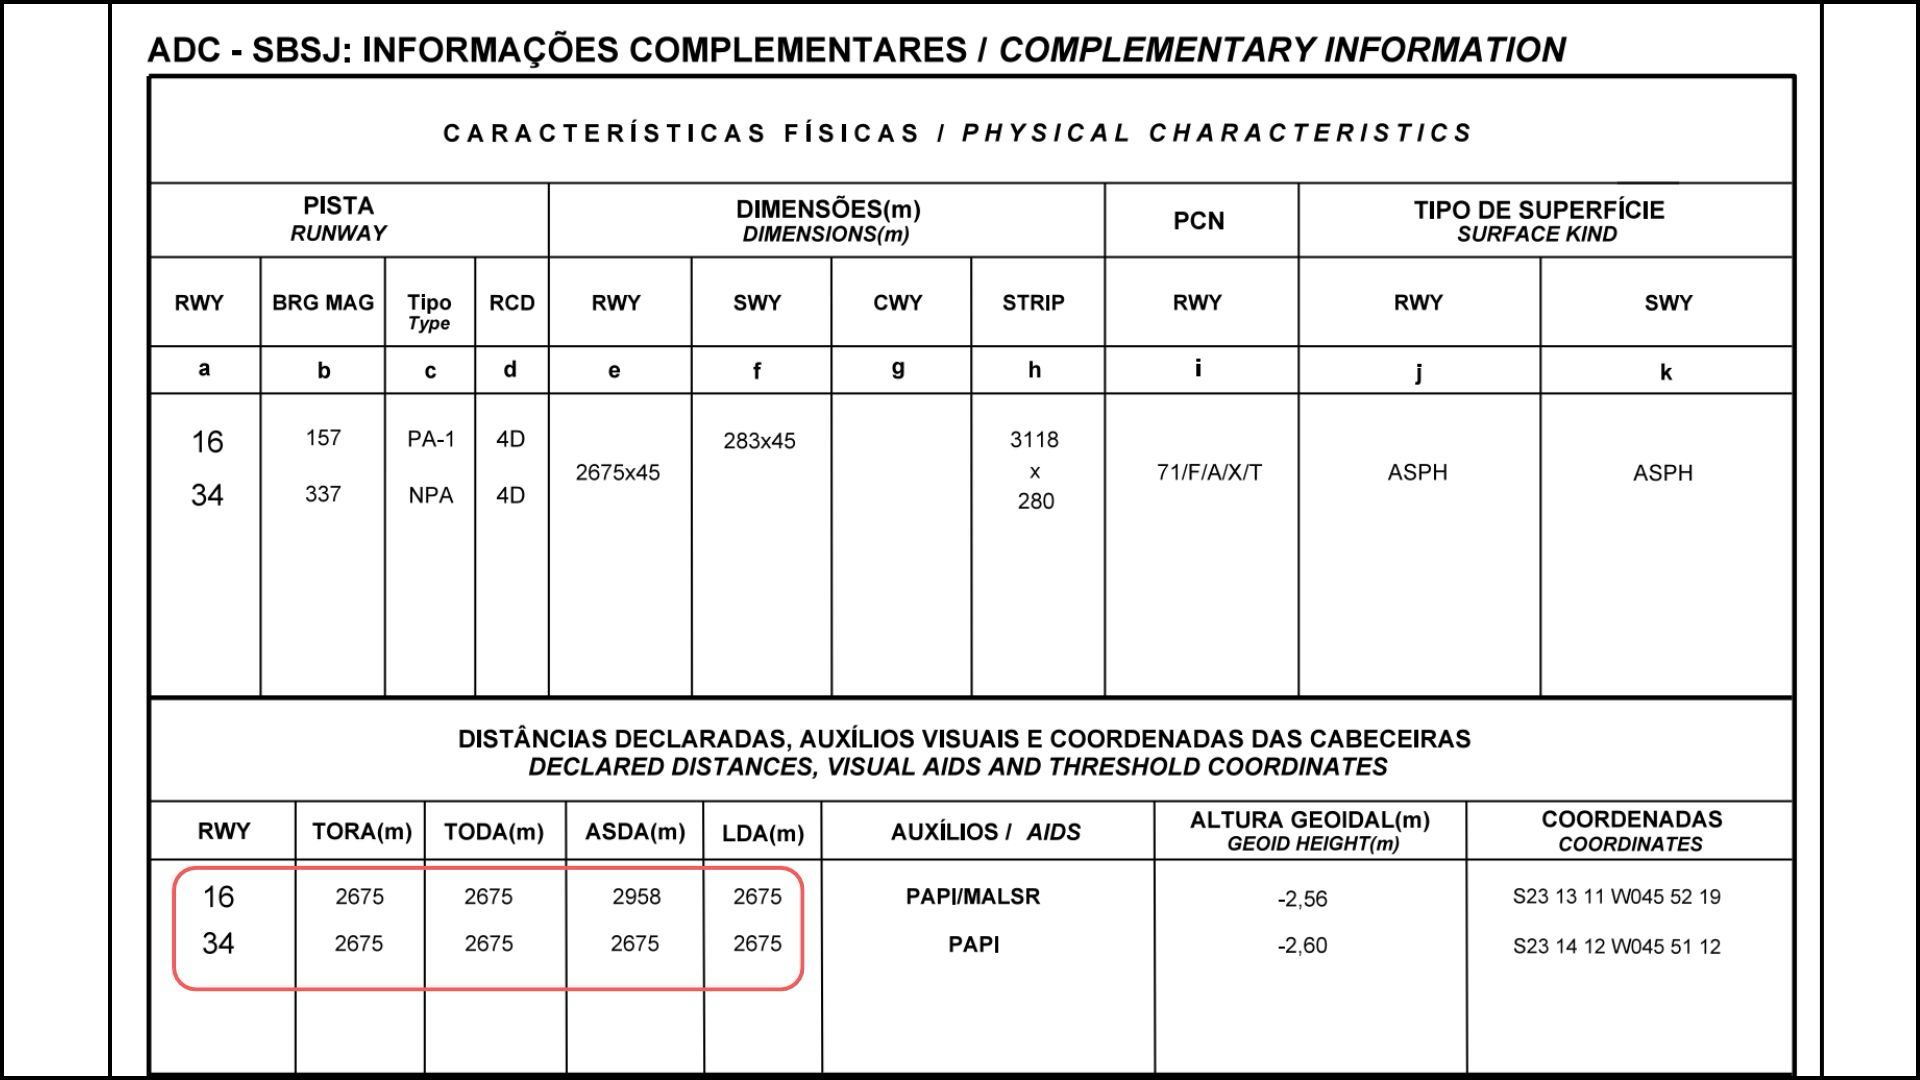
\includegraphics[width=0.9\linewidth]{Figures/ADC_SBSJ.png}
        \caption{ADC, emenda AIRAC 2604 (2026): informações complementares.}
        \label{fig:adc}
    \end{subfigure}

    \bigskip
    \begin{subfigure}{\linewidth}
        \centering
        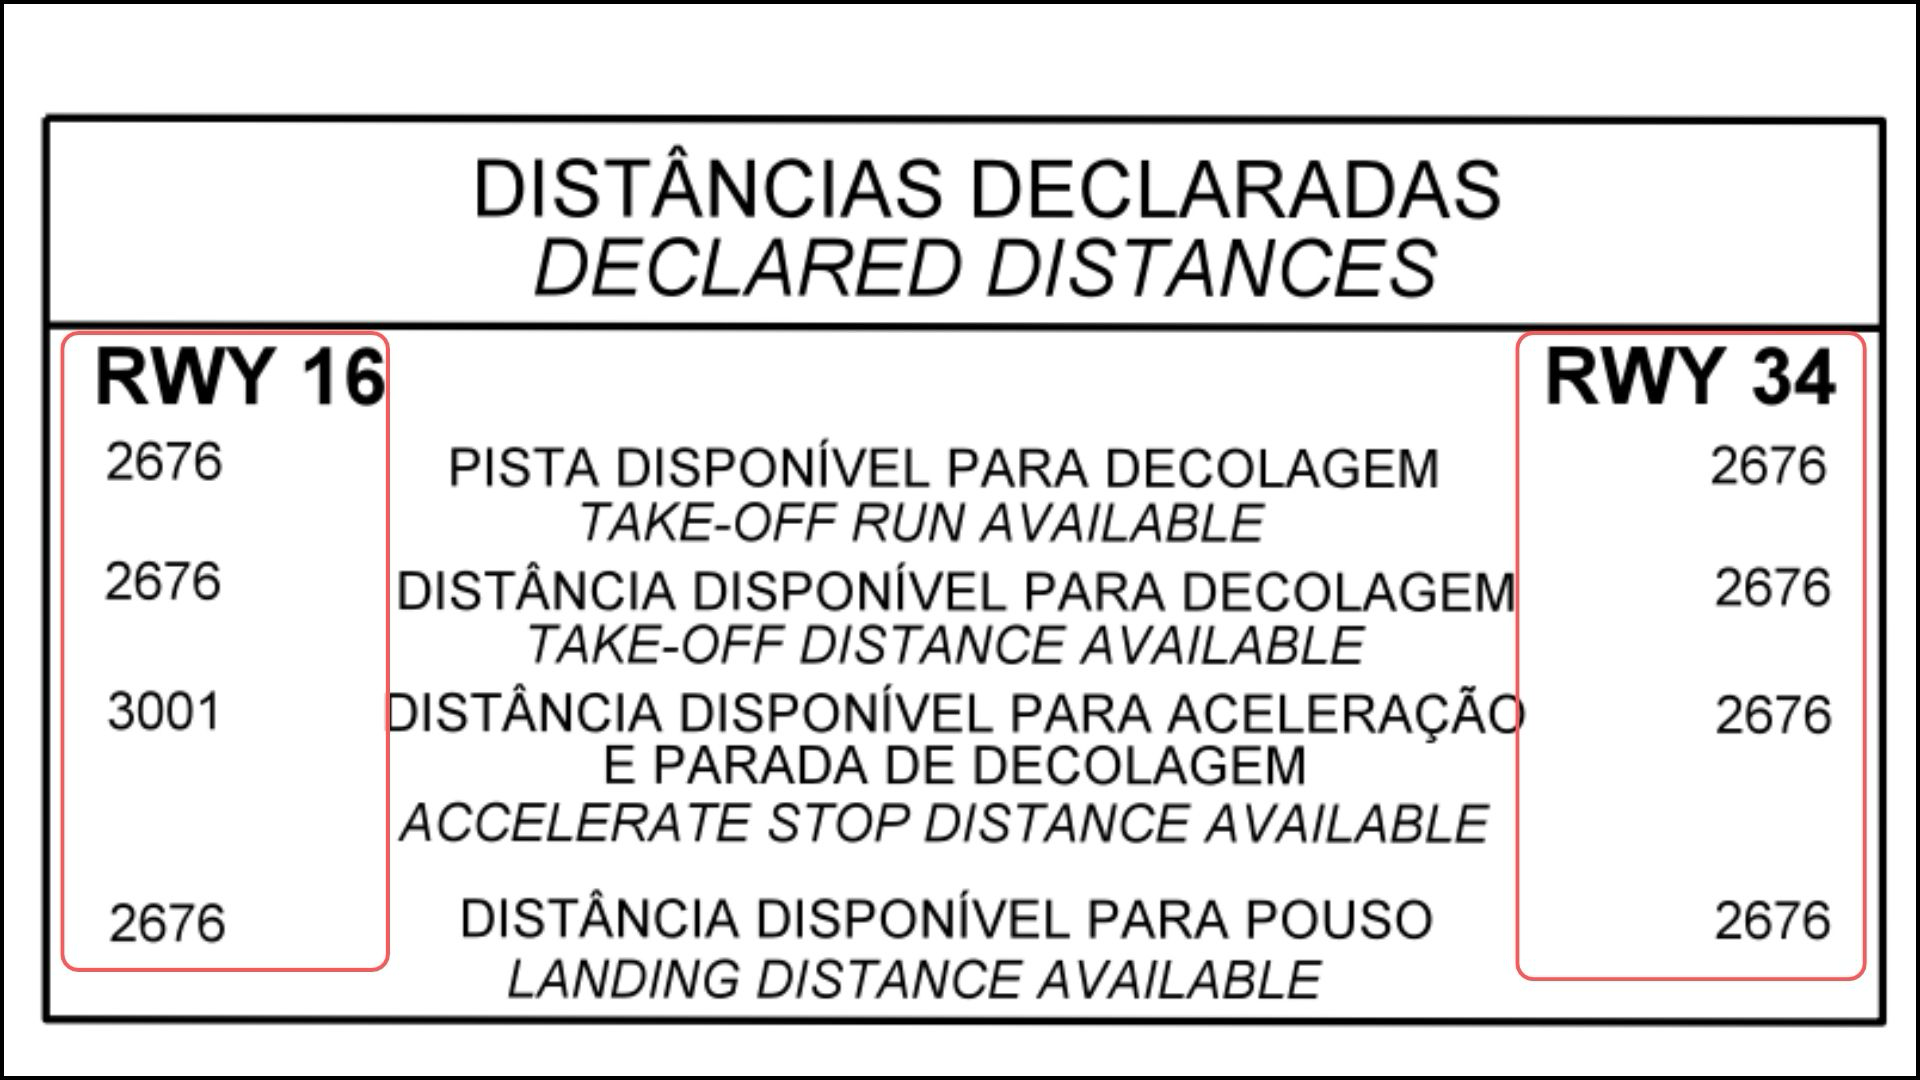
\includegraphics[width=0.5\linewidth]{Figures/AOC_SBSJ_pista.png}
        \caption{AOC, emenda AIRAC 2213 (2022): distâncias declaradas.}
        \label{fig:aoc-dist}
    \end{subfigure}

    \bigskip
    \begin{subfigure}{\linewidth}
        \centering
        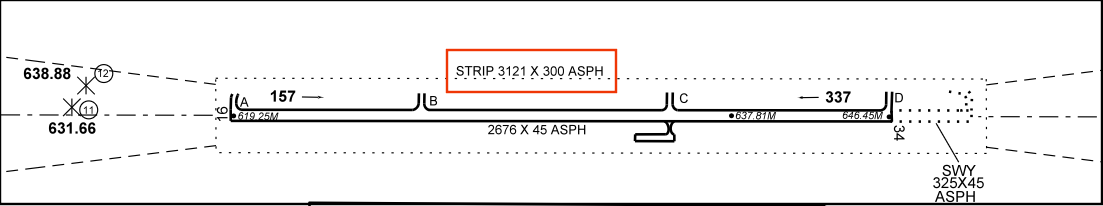
\includegraphics[width=0.9\linewidth]{Figures/AOC_SBSJ_distancia_declarada.png}
        \caption{AOC, emenda AIRAC 2213 (2022): dimensões em planta.}
        \label{fig:aoc-planta}
    \end{subfigure}

    \caption{Dimensões e distâncias declaradas da pista do SBSJ em duas cartas
    oficiais.}
    \label{fig:adc-aoc}

    \medskip
    {\small Fonte: DECEA, AIP Brasil (cartas completas nos Anexos~\ref{anexo:adc}
    e~\ref{anexo:aoc}).}
\end{figure}

A divergência pode decorrer, em parte, de as duas cartas terem propósitos distintos. Enquanto a AOC reúne as informações sobre obstáculos necessárias ao cálculo de desempenho na decolagem, a ADC apoia a movimentação das aeronaves no aeródromo \cite{icao_anexo4}. Além disso, foram emitidas com quatro anos de intervalo e, nesse período, podem ter ocorrido novos levantamentos, obras na pista, correções ou mudanças nos critérios de cálculo. A prática de adotar a publicação mais recente como vigente é, nesse contexto, adequada.

Nenhum dos documentos informa o que motivou a alteração, quem a realizou ou de quais medições e critérios os novos valores dependem. Esse conhecimento possivelmente existe no órgão responsável pelas publicações, mas não acompanha os dados publicados. Além disso, reconstruir o que estava publicado em uma data passada depende de que o usuário tenha conservado a edição correspondente. No caso do SBSJ, a comparação só foi possível porque ambas as cartas permaneciam disponíveis.

O problema abordado neste trabalho é, portanto, de rastreabilidade. Busca-se garantir que, para qualquer valor publicado, seja possível:
\begin{itemize}
    \item identificar a sua origem, as premissas de que depende e a causa de cada alteração;
    \item reconstruir o estado dos dados em qualquer instante;
    \item verificar que esse histórico não foi modificado.
\end{itemize}

Para tratar esse problema, este trabalho propõe uma arquitetura de dados em que cada alteração é registrada como um evento imutável, com autor e causa declarados. Os valores que podem ser calculados a partir de outros, como comprimentos e distâncias declaradas, não são armazenados: são derivados das premissas no momento da consulta. O princípio é o mesmo dos registros contábeis, em que nenhum lançamento é apagado e um erro é corrigido por um novo lançamento, com motivo declarado \cite{helland2016}. Os fundamentos dessa abordagem e a sua relação com os modelos de informação aeronáutica existentes são apresentados no Capítulo~\ref{chap:fundamentacao}.

\section{Objetivos}

Este trabalho busca responder à seguinte pergunta:

\begin{quote}
Em que medida uma arquitetura baseada em \textit{event sourcing} torna auditáveis os dados geolocalizados de infraestrutura aeroportuária, e quais são os limites dessa auditabilidade?
\end{quote}

A hipótese é que essa arquitetura permite que tais dados sejam:
\begin{itemize}
    \item rastreáveis até a sua causa;
    \item recalculáveis a partir das premissas;
    \item reconstruíveis no tempo;
    \item consistentes entre produtos;
    \item protegidos por evidência de adulteração.
\end{itemize}
Os limites da auditabilidade não são presumidos: resultam dos experimentos e das restrições declaradas pela própria implementação.

\subsection{Objetivo geral}

Propor e avaliar uma arquitetura de dados baseada em \textit{event sourcing} que torne auditáveis os dados geolocalizados de infraestrutura aeroportuária, identificando os limites dessa auditabilidade. O escopo restringe-se à estrutura física de uma pista, embora a arquitetura admita extensão a dados operacionais.

\subsection{Objetivos específicos}

\begin{itemize}
    \item Caracterizar a lacuna de rastreabilidade nas publicações aeronáuticas, a partir das diferenças entre as cartas oficiais do SBSJ e dos requisitos do PANS-AIM.
    \item Propor uma arquitetura em que cada alteração seja registrada como evento imutável, com autor e causa declarados e encadeado por \textit{hash}. Nela, a geometria é representada pelas premissas que a geram, e os valores derivados são calculados no momento da consulta.
    \item Implementar a arquitetura como biblioteca de código aberto, independente do experimento que a avalia.
    \item Avaliar a arquitetura por meio de seis experimentos sobre a pista do SBSJ, com dados reais, cada um dedicado a uma propriedade e com critérios de aprovação definidos antes da execução.
    \item Identificar os limites da auditabilidade obtida, distinguindo o que os experimentos demonstram do que é apenas argumentado.
\end{itemize}

\section{Organização do trabalho}

O Capítulo~\ref{chap:fundamentacao} apresenta os fundamentos em que o trabalho se apoia, isto é, os padrões de informação aeronáutica e geoespacial e os modelos de dados que retêm histórico, em especial nos sistemas financeiros. O Capítulo~\ref{chap:metodologia} descreve o método, com os requisitos que a solução deve atender, o estudo de caso e os experimentos que a avaliam. O Capítulo~\ref{chap:solucao} desenvolve a arquitetura proposta, a sua implementação e a sua aplicação ao SBSJ. O Capítulo~\ref{chap:resultados} apresenta os resultados dos experimentos, e o Capítulo~\ref{chap:discussao} os discute, junto com os limites identificados. O Capítulo~\ref{chap:conclusao} apresenta as conclusões e os trabalhos futuros.


\chapter{Fundamentação teórica}\label{chap:fundamentacao}
Este capítulo apresenta os fundamentos em que o trabalho se apoia. A Seção~\ref{sec:info-aero} trata da informação aeronáutica, isto é, de como é publicada, que requisitos de qualidade deve atender e como os modelos de intercâmbio a representam. A Seção~\ref{sec:geo} apresenta o referenciamento linear e os conceitos de geodésia necessários para calcular comprimentos a partir de posições medidas. As Seções~\ref{sec:temporal} a~\ref{sec:adulteracao} tratam dos modelos de dados que retêm histórico: os bancos de dados temporais, o padrão \textit{event sourcing}, os registros imutáveis dos sistemas financeiros e os mecanismos de evidência de adulteração. A Seção~\ref{sec:distribuidos} discute os compromissos entre consistência e disponibilidade em sistemas distribuídos, e a Seção~\ref{sec:sintese-fund} relaciona esses fundamentos às escolhas deste trabalho.

\section{Informação aeronáutica}\label{sec:info-aero}

\subsection{Produtos, ciclo AIRAC e qualidade dos dados}\label{sec:produtos}

O Anexo~15 à Convenção de Aviação Civil Internacional e os Procedimentos para os Serviços de Navegação Aérea -- Gestão da Informação Aeronáutica (PANS-AIM) organizam a informação aeronáutica em produtos \cite{icao2018anexo15,icao2018pansaim}. Entre eles estão a Publicação de Informação Aeronáutica (AIP), com as suas emendas e suplementos, os NOTAM, as cartas aeronáuticas e, de forma crescente, os conjuntos de dados digitais. As alterações operacionalmente significativas seguem o ciclo AIRAC (\textit{Aeronautical Information Regulation and Control}). Nesse ciclo, as datas de efetividade são comuns a todos os Estados e espaçadas de 28 dias, e a publicação ocorre com antecedência mínima de 42 dias, para que os usuários possam se preparar antes da entrada em vigor. Cada emenda substitui o conteúdo afetado da edição anterior, assim, O produto publicado representa o estado dos dados na sua data de efetividade.

O Anexo~4 define o propósito de cada carta aeronáutica \cite{icao_anexo4}. A Carta de Obstáculos de Aeródromo -- Tipo~A (AOC) fornece ao operador os dados de obstáculos necessários para cumprir as limitações de desempenho na decolagem. A Carta de Aeródromo (ADC) reúne as informações que facilitam a movimentação das aeronaves no solo, entre as posições de estacionamento e a pista, além de informações operacionais essenciais do aeródromo. Os dois produtos compartilham parte dos dados, como o comprimento da pista e as distâncias declaradas. Cada um, porém, os apresenta segundo a sua finalidade e na data da sua própria emenda.

O Anexo~15 e o PANS-AIM estabelecem requisitos de qualidade para os dados aeronáuticos, que abrangem exatidão, resolução, integridade, rastreabilidade, oportunidade, completude e formato \cite{icao2018anexo15,icao2018pansaim}. Dois desses requisitos interessam diretamente a este trabalho, dentre deles a integridade, que é o grau de garantia de que um dado e o seu valor não foram perdidos nem alterados desde a sua origem ou desde uma emenda autorizada. Os dados são classificados em rotineiros, essenciais e críticos, conforme o risco associado ao seu uso incorreto. Outro requisito é a rastreabilidade, que é a capacidade de reconstituir a história, a aplicação ou a localização daquilo que se considera, e deve ser assegurada ao longo de toda a cadeia de dados. O PANS-AIM exige, além disso, consistência entre os produtos de informação aeronáutica.

Esses requisitos recaem sobre os provedores do serviço e sobre a sua cadeia de produção. O produto que chega ao usuário, contudo, apresenta os valores vigentes sem carregar a trilha que permitiria reconstituí-los.

\subsection{Distâncias declaradas}\label{sec:distancias}

O Anexo~14 define as distâncias declaradas de uma pista, que correspondem aos comprimentos disponíveis para cada fase da operação e são publicadas para cada direção de pista \cite{icao2022anexo14}. A distância disponível para corrida de decolagem (TORA, \textit{take-off run available}) é o comprimento de pista declarado disponível e adequado para a corrida no solo de uma aeronave em decolagem. A distância disponível para decolagem (TODA, \textit{take-off distance available}) acrescenta à TORA o comprimento da zona livre de obstáculos (\textit{clearway}, CWY), quando houver. De modo análogo, a distância disponível para aceleração e parada (ASDA, \textit{accelerate-stop distance available}) acrescenta à TORA o comprimento da zona de parada (\textit{stopway}, SWY). A distância disponível para pouso (LDA, \textit{landing distance available}) é o comprimento de pista declarado disponível e adequado para a corrida no solo de uma aeronave em pouso.

A zona de parada é uma área retangular além do fim da TORA, preparada para que uma aeronave possa parar em caso de decolagem abortada. Sobre a zona livre de obstáculos, a aeronave pode completar parte da subida inicial. Quando a cabeceira é deslocada, a LDA é reduzida do comprimento do deslocamento. As distâncias declaradas não são, portanto, medidas independentes. Elas resultam do comprimento da pista, das dimensões dessas áreas e da posição das cabeceiras, segundo regras normativas. A Figura~\ref{fig:distancias} mostra essas definições em uma direção de pista e a dependência de cada distância em relação às suas premissas.

\begin{figure}[htbp]
    \centering
    \begin{subfigure}{\linewidth}
        \centering
        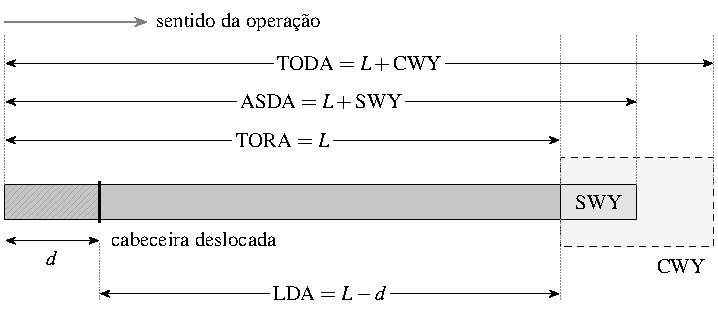
\includegraphics[page=1]{Figures/fig_distancias_declaradas.pdf}
        \caption{Esquema de uma direção de pista, fora de escala.}
        \label{fig:distancias-esquema}
    \end{subfigure}

    \bigskip
    \begin{subfigure}{\linewidth}
        \centering
        \includegraphics[page=2]{Figures/fig_distancias_declaradas.pdf}
        \caption{Dependência entre as premissas e as distâncias declaradas.}
        \label{fig:distancias-dependencia}
    \end{subfigure}

    \caption{Distâncias declaradas de uma direção de pista, segundo as definições do Anexo~14.}
    \label{fig:distancias}
    \par\smallskip{\small Fonte: o autor, a partir de \citeonline{icao2022anexo14}.}
\end{figure}

A Figura~\ref{fig:distancias} mostra essas definições em uma direção de pista e a dependência de cada distância em relação às suas premissas.

\begin{figure}[htbp]
    \centering
    \begin{subfigure}{\linewidth}
        \centering
        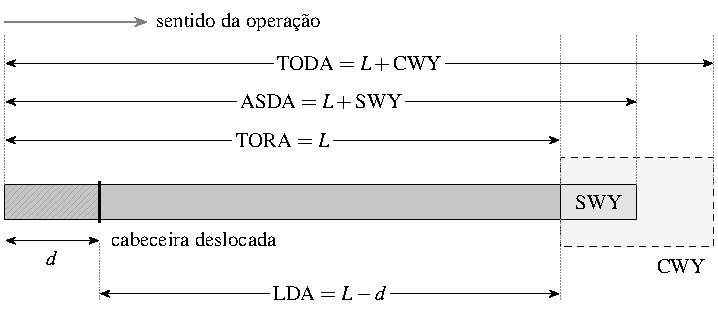
\includegraphics[page=1]{Figures/fig_distancias_declaradas.pdf}
        \caption{Esquema de uma direção de pista, fora de escala.}
        \label{fig:distancias-esquema}
    \end{subfigure}

    \bigskip
    \begin{subfigure}{\linewidth}
        \centering
        \includegraphics[page=2]{Figures/fig_distancias_declaradas.pdf}
        \caption{Dependência entre as premissas e as distâncias declaradas.}
        \label{fig:distancias-dependencia}
    \end{subfigure}

    \caption{Distâncias declaradas de uma direção de pista, segundo as definições do Anexo~14.}
    \label{fig:distancias}
    \par\smallskip{\small Fonte: o autor, a partir de \citeonline{icao2022anexo14}.}
\end{figure}

\subsection{AIXM}\label{sec:aixm}

O AIXM (\textit{Aeronautical Information Exchange Model}) é o modelo de referência para o intercâmbio digital de informação aeronáutica, desenvolvido pela EUROCONTROL e pela \textit{Federal Aviation Administration} (FAA). O modelo tem dois componentes: O primeiro é um modelo lógico em UML, com as entidades necessárias à navegação aérea, enquanto o segundo é um esquema XML baseado em GML, para a troca de dados entre sistemas \cite{eurocontrol2016aixm}. A versão 5.1.1 é a mais usada em operação.

O aspecto do AIXM mais relevante para este trabalho é o seu modelo de temporalidade \cite{eurocontrol2021temporality}. Cada \textit{Feature}, como uma pista ou uma cabeceira, tem identidade própria e é descrita por uma sequência de \textit{TimeSlices}, cada uma com um período de validade e uma interpretação. A interpretação \texttt{BASELINE} descreve o estado completo a partir de um instante, e \texttt{PERMDELTA}, uma alteração permanente. \texttt{TEMPDELTA} descreve uma alteração temporária, como a de um NOTAM, que se sobrepõe ao estado de base e expira. \texttt{SNAPSHOT}, por fim, apresenta o estado resultante em um instante, para consulta. Cada \textit{TimeSlice} traz ainda um \texttt{sequenceNumber}, que ordena as versões, e um \texttt{correctionNumber}, que identifica correções de uma versão já emitida. Os dados podem ser acompanhados de anotações em texto livre.

O AIXM tem, portanto, noção de tempo e uma disciplina de correção, mas há três aspectos que ele não garante. O primeiro é a retenção do histórico; o modelo permite representar versões e correções, mas não obriga quem publica a mantê-las, e um serviço de consulta pode devolver apenas o estado corrente. O segundo é a evidência de adulteração, já que nada no modelo permite a quem recebe os dados verificar que uma versão antiga não foi alterada depois de publicada. O terceiro é o registro das premissas e da causa de cada mudança, dessa forma, valores como as distâncias declaradas são publicados como números, sem indicação das medições que os originaram, e a razão de uma alteração, quando existe, fica em texto livre.

\subsection{Ferramentas de projeto e de SIG}\label{sec:sig}

Ferramentas de projeto, como CAD e BIM, e sistemas de informação geográfica (SIG) são as fontes mais comuns dos dados aeroportuários. O \textit{ArcGIS Aviation Airports}, da Esri, por exemplo, gera superfícies limitadoras de obstáculos de forma paramétrica, a partir do eixo e da classificação da pista, e exporta dados em AIXM \cite{esri2024}. Nessas ferramentas, o resultado do cálculo é persistido como dado primário, e é a superfície gerada, ou o desenho, que se guarda e se distribui. A relação entre esse resultado e as medições que o originaram não fica registrada, e quando existe versionamento, ele é feito sobre arquivos ou tabelas, sem registro estruturado da causa de cada alteração.

\section{Referenciamento linear e geodésia}\label{sec:geo}

\subsection{Referenciamento linear (ISO 19148)}\label{sec:iso19148}

A ISO~19148 define como expressar posições ao longo de elementos lineares, independentemente do sistema de coordenadas \cite{iso19148}. Nesse modelo, o elemento linear estabelece a direção de medição, e um referente (\textit{Referent}), ponto conhecido sobre o elemento, estabelece a origem. A posição é então dada pela distância ao longo do elemento (\textit{DistanceExpression}) e pelos afastamentos lateral e vertical em relação a ele (\textit{LateralOffsetExpression} e \textit{VerticalOffsetExpression}). Na forma geral,
\begin{equation}
    p = f(e,\, r,\, s,\, o,\, v)
    \label{eq:lrs}
\end{equation}
em que $e$ é o elemento linear, $r$ o referente, $s$ a distância ao longo do elemento, $o$ o afastamento lateral e $v$ o afastamento vertical.

O referenciamento linear é usado há décadas em rodovias e ferrovias, em que a posição de um elemento é expressa por um marco quilométrico e um afastamento. As posições, nesse modelo, não guardam coordenadas próprias, e sim uma relação com o referente. Uma nova medição do referente desloca, assim, todas as posições que dependem dele, sem que nenhuma delas precise ser reescrita.

\subsection{Distâncias sobre o elipsoide}\label{sec:geodesia}

Coordenadas geográficas são expressas em relação a um referencial geodésico. No Brasil, o referencial oficial é o SIRGAS2000 \cite{ibge2005sirgas}, que adota o elipsoide GRS80. Sobre o elipsoide, a menor distância entre dois pontos é a geodésica, cujo comprimento e cujos azimutes nas extremidades se obtêm pelo problema geodésico inverso. \citeonline{vincenty1975} resolve esse problema por iteração, com exatidão da ordem de 0,5~mm. \citeonline{karney2013} apresenta um algoritmo com exatidão próxima à da aritmética de ponto flutuante e convergência garantida em todos os casos.

A altitude também depende de uma referência. A altitude elipsoidal $h$, obtida por posicionamento por satélite, relaciona-se com a altitude ortométrica $H$, referida ao geoide, pela ondulação geoidal $N$:
\begin{equation}
    h = H + N
    \label{eq:ondulacao}
\end{equation}
As cartas de aeródromo publicam a elevação das cabeceiras e a ondulação geoidal, o que permite passar de uma referência à outra.

Projeções cartográficas, como a Universal Transversa de Mercator (UTM), representam o elipsoide em um plano à custa de deformações. Na UTM, o fator de escala vale 0,9996 no meridiano central de cada fuso e varia com o afastamento a ele. O norte da quadrícula, além disso, não coincide com o norte verdadeiro, e a diferença entre eles é a convergência meridiana. Distâncias e azimutes medidos sobre a projeção diferem, portanto, dos medidos sobre o elipsoide, e a diferença varia com a posição.

Um comprimento calculado sobre o elipsoide tampouco coincide com o comprimento medido sobre o terreno, e duas reduções os relacionam. A primeira é a de altitude. Uma distância horizontal $D_h$, medida à altitude $h$, corresponde no elipsoide a
\begin{equation}
    D_0 = D_h \frac{R}{R + h} \approx D_h \left(1 - \frac{h}{R}\right)
    \label{eq:reducao-altitude}
\end{equation}
em que $R$ é o raio de curvatura da Terra no local. A segunda é a de inclinação. Entre dois pontos com desnível $\Delta z$ e distância horizontal $L$, a distância inclinada excede a horizontal em aproximadamente
\begin{equation}
    \Delta L \approx \frac{\Delta z^2}{2L}
    \label{eq:reducao-inclinacao}
\end{equation}
Um produto que publique comprimentos precisa, portanto, declarar a convenção adotada. Sem essa declaração, dois valores corretos para a mesma pista podem diferir apenas por convenção.

\section{Dados temporais}\label{sec:temporal}

\subsection{Tempo de validade e tempo de transação}\label{sec:bitemporal}

A retenção do histórico de um banco de dados, e não apenas do seu estado corrente, é estudada há décadas na área de bancos de dados temporais. \citeonline{snodgrass2000} distingue dois eixos de tempo. O tempo de validade corresponde ao período em que um fato é verdadeiro no mundo, e o tempo de transação, ao instante em que o fato foi registrado no banco. Um banco que mantém os dois eixos é chamado bitemporal.

A distinção tem consequências diferentes conforme o domínio. Em uma transação financeira, o lançamento registrado constitui o próprio fato para fins contábeis, e o saldo de uma conta não descreve nenhum objeto independente do sistema. Os dados aeronáuticos, ao contrário, descrevem objetos físicos que existem independentemente da sua representação. Uma pista existe antes de ser medida ou publicada, e a sua medição pode ser registrada dias ou meses depois de realizada, além de poder estar incorreta.

Considere uma pista cujo comprimento sempre foi de 2500~m, mas que foi publicada durante anos com o valor de 2600~m. Quando o erro é identificado, registra-se uma correção, e o histórico admite duas leituras. Com apenas o tempo de transação, o sistema informa que o valor publicado era de 2600~m até a data da correção, o que permite reconstruir o que foi oficialmente informado em cada instante. Com os dois eixos, o sistema representa, ao mesmo tempo, que a pista sempre teve 2500~m e que o registro informava 2600~m até determinada data. A primeira leitura atende à auditoria documental, enquanto a segunda permite também relacionar ocorrências passadas a uma condição que só foi reconhecida depois.

\subsection{Event sourcing e CQRS}\label{sec:event-sourcing}

\citeonline{fowler2005} descreve o padrão \textit{event sourcing}, que leva a retenção do histórico ao seu limite, e nele, o estado não é gravado, mas derivado da sequência de eventos que o produziu. Cada alteração é um evento acrescentado a um registro em que só se escreve, e o estado em qualquer instante é obtido reprocessando os eventos até ele.

O padrão costuma vir acompanhado da segregação entre comandos e consultas (CQRS, \textit{Command Query Responsibility Segregation}), descrita por \citeonline{young2010}. O lado da escrita valida os comandos e registra os eventos. O lado da leitura monta, a partir deles, tantos modelos de consulta quantos forem necessários, todos descartáveis e reconstruíveis. \citeonline{kleppmann2017} mostra como esse modelo, em que um registro ordenado é a fonte da verdade e os demais dados são derivados dele, sustenta sistemas de dados de grande porte.

\section{Registros imutáveis em sistemas financeiros}\label{sec:financeiro}

O registro de eventos imutáveis é a base de sistemas financeiros em produção, nos quais a exigência de auditoria é antiga e o volume de operações é muito maior que o da informação aeronáutica. Em um livro-razão, nenhum lançamento é apagado, um erro é corrigido por um lançamento de estorno e o saldo é derivado dos lançamentos \cite{helland2016}. Dessa forma, empresas de pagamento aplicam esse princípio diretamente, como mostram os registros de movimentação de dinheiro da Stripe \cite{ganelin2024} e da Square \cite{strzalkowski2019}.

\citeonline{fowler2011} descreve o núcleo da LMAX, uma bolsa de negociação de varejo. Toda a lógica de negócio é executada em memória, em uma única \textit{thread}, e processa cerca de seis milhões de pedidos por segundo, o estado, no entanto, não é persistido diretamente. Cada evento de entrada é gravado em um diário (\textit{journal}) antes de ser processado, e, em caso de falha, o estado é reconstruído reprocessando esses eventos a partir do último \textit{snapshot}. O caso mostra que a reconstrução do estado a partir de eventos é um mecanismo de operação, e não apenas de laboratório, e que o seu custo de escrita não é impeditivo.

Nenhum dos dois casos trata, porém, da evidência de adulteração e não permitem que um terceiro verifique que eles não foram alterados. Essa garantia vem de outra linha de trabalho, tratada a seguir.

\section{Evidência de adulteração}\label{sec:adulteracao}

\citeonline{haber1991} propõem encadear registros por funções de \textit{hash}. Cada registro inclui o \textit{hash} do anterior, de modo que alterar qualquer um deles invalida todos os elos seguintes. A mesma ideia sustenta os bancos de dados de \textit{ledger}, que guardam o histórico de forma verificável. \citeonline{antonopoulos2021} descrevem o SQL Ledger, do Azure SQL Database, que mantém as tabelas comuns do banco, mas encadeia criptograficamente cada transação. O sistema também publica resumos (\textit{digests}) que permitem verificar, posteriormente, que nada foi alterado.

Esse mecanismo tem um limite. A cadeia detecta alterações pontuais, mas não a reescrita completa do registro por quem o controla, que produz uma nova sequência internamente coerente. Essa reescrita só é detectada se um resumo anterior do registro, como o \textit{hash} do último elo (a cabeça da cadeia), tiver sido guardado fora do sistema, na forma de uma âncora externa. É por essa razão que o SQL Ledger publica os seus resumos em armazenamento externo e imutável.

\section{Consistência e disponibilidade em sistemas distribuídos}\label{sec:distribuidos}

Quando os dados são replicados para vários leitores, surge um compromisso conhecido. \citeonline{brewer2000} formula o teorema CAP, que \citeonline{gilbert2002} demonstram formalmente. Segundo o teorema, um sistema distribuído, diante de uma partição da rede, precisa escolher entre consistência e disponibilidade. Ou responde sempre, ainda que com dados possivelmente desatualizados, ou responde sempre de forma consistente, ainda que às vezes deixe de responder.

\citeonline{kleppmann2017} mostra que esse compromisso pode ser resolvido de forma diferente em cada parte de um sistema construído sobre um registro ordenado. A escrita pode ser centralizada em um único ponto, que impõe a ordem total dos eventos, enquanto a leitura é distribuída entre consumidores que mantêm as suas próprias cópias derivadas. A transferência dos eventos do banco para os consumidores é feita por captura de mudanças (\textit{change data capture}, CDC), seja pela leitura do registro do banco, seja por uma tabela de saída (\textit{outbox}) gravada na mesma transação. Cada consumidor guarda apenas a sua posição de leitura. Como o registro só cresce, um consumidor atrasado conhece um prefixo do registro, e nunca uma versão divergente dele.

\section{Síntese}\label{sec:sintese-fund}

Os fundamentos apresentados delimitam o espaço em que este trabalho se situa. A informação aeronáutica já dispõe de requisitos de integridade e rastreabilidade e de um modelo de intercâmbio com noção de tempo, mas nenhum dos dois assegura que o histórico, as premissas e a causa de cada alteração cheguem ao usuário junto com os dados. As distâncias declaradas, por sua vez, decorrem de regras do Anexo~14 aplicadas a posições e dimensões, o que as torna candidatas naturais a valores calculados, e não armazenados. O referenciamento linear da ISO~19148 e a geodésia sobre o elipsoide oferecem os meios para registrar posições por dependência e para calcular comprimentos sob uma convenção explícita.

Dos modelos que retêm histórico, este trabalho adota o \textit{event sourcing} e a separação entre escrita e leitura, com o tempo de transação como única linha do tempo e a bitemporalidade como extensão possível. Dos sistemas financeiros, adota o princípio do livro-razão, em que nada se apaga e toda correção é um novo registro. Da linha de evidência de adulteração, adota o encadeamento por \textit{hash}, com a cadeia linear pelo pequeno volume do domínio, e reconhece o limite que só uma âncora externa supera. A discussão sobre sistemas distribuídos, por fim, fundamenta a escolha de privilegiar a consistência na escrita e a disponibilidade na leitura. O Capítulo~\ref{chap:metodologia} parte desses fundamentos para definir os requisitos do artefato e o método pelo qual ele é avaliado.


\chapter{Metodologia}\label{chap:metodologia}
Este capítulo descreve como o trabalho foi conduzido e como a proposta é avaliada. A Seção~\ref{sec:dsr} apresenta a abordagem de pesquisa. A Seção~\ref{sec:requisitos} define os requisitos que a solução deve atender, antes de qualquer escolha de arquitetura. A Seção~\ref{sec:caso} apresenta o estudo de caso e os dados utilizados, e a Seção~\ref{sec:experimentos}, os experimentos e os seus critérios de aprovação. As Seções~\ref{sec:validacao} e~\ref{sec:reprodutibilidade} tratam, por fim, de como a avaliação evita conferir a solução contra ela mesma e de como pode ser reproduzida.

\section{Abordagem de pesquisa}\label{sec:dsr}

O trabalho segue a pesquisa em ciência do design (\textit{design science research}, DSR), em que o conhecimento resulta da construção e da avaliação de um artefato dirigido a um problema identificado \cite{hevner2004}. O artefato, aqui, é a arquitetura de dados e a sua implementação. As etapas adotadas são as propostas por \citeonline{peffers2007}, e a Tabela~\ref{tab:dsr-etapas} indica onde cada uma é tratada.

\begin{table}[htbp]
    \centering
    \caption{Etapas da pesquisa em ciência do design e a sua localização no trabalho.}
    \label{tab:dsr-etapas}
    \begin{tabularx}{\linewidth}{X l}
        \toprule
        Etapa & Onde é tratada \\
        \midrule
        Identificação do problema e motivação & Capítulo~\ref{chap:introducao} \\
        Definição dos objetivos da solução & Seção~\ref{sec:requisitos} \\
        Projeto e desenvolvimento do artefato & Seções~\ref{sec:visao-geral} a~\ref{sec:implementacao} \\
        Demonstração & Seção~\ref{sec:aplicacao-sbsj} \\
        Avaliação & Seção~\ref{sec:experimentos} e Capítulo~\ref{chap:resultados} \\
        Comunicação & este texto, a biblioteca e o banco extraído \\
        \bottomrule
    \end{tabularx}
    \par\smallskip{\small Fonte: o autor, a partir de \citeonline{peffers2007}.}
\end{table}

A avaliação é feita por falseamento. Cada propriedade da hipótese é traduzida em uma pergunta de resposta sim ou não, com um critério de aprovação fixado antes da execução. Um experimento reprovado refutaria a propriedade correspondente no caso estudado. Um experimento aprovado não a prova em geral, mas mostra que a arquitetura a sustenta nas condições declaradas.

\section{Requisitos do artefato}\label{sec:requisitos}

Os requisitos descrevem um serviço de dados auditável como uma caixa-preta, isto é, pelas perguntas que ele precisa responder, e não pela forma como as responde. Definidos antes da arquitetura, eles evitam que a solução proposta justifique o próprio problema. A Tabela~\ref{tab:requisitos} os resume, e as subseções seguintes os detalham. O Capítulo~\ref{chap:solucao} mostra, depois, o mecanismo que atende a cada um.

\begin{table}[htbp]
    \centering
    \caption{Requisitos de um serviço de dados auditável.}
    \label{tab:requisitos}
    \begin{tabularx}{\linewidth}{l X}
        \toprule
        Requisito & O serviço deve \\
        \midrule
        R1 Origem de cada valor & informar quem afirmou cada valor, por quê e com base em quais premissas \\
        R2 Reconstrução no tempo & reconstruir o conteúdo de qualquer produto em qualquer instante passado \\
        R3 Consistência entre produtos & impedir que dois produtos referentes ao mesmo instante divirjam \\
        R4 Mínimo de informação & guardar apenas o que não pode ser calculado a partir de outros dados \\
        R5 Posição relativa & registrar posições em relação a pontos medidos, de modo que uma nova medição se propague \\
        R6 Estrutura comum e conteúdo flexível & exigir uma forma mínima comum a todos os elementos e aceitar o restante sem esquema fixo \\
        R7 Verificação por terceiro & permitir que quem recebe os dados confira a sua integridade sem confiar em quem os publica \\
        \bottomrule
    \end{tabularx}
    \par\smallskip{\small Fonte: o autor.}
\end{table}

\subsection{R1: origem de cada valor}\label{sec:req-origem}

O serviço deve informar, para cada valor, quem o afirmou, por que motivo e com base em quais premissas. Essa é a pergunta central de uma auditoria e a que as publicações atuais não respondem (Capítulo~\ref{chap:introducao}). Um valor sem autor e sem causa pode estar correto, mas não pode ser auditado.

\subsection{R2: reconstrução no tempo}\label{sec:req-tempo}

O serviço deve reconstruir o conteúdo de qualquer produto em qualquer instante passado, sem depender de que o usuário tenha guardado a edição correspondente. Este trabalho adota um único eixo de tempo, o de transação (Seção~\ref{sec:bitemporal}), por dois motivos. O primeiro é documental. O que se pretende auditar é o que foi oficialmente afirmado em cada instante, e o tempo de transação responde exatamente a isso. O segundo é metodológico. O segundo eixo traz complexidade própria, como a consulta em duas dimensões e o fim de validade calculável apenas na leitura, que exigiria uma avaliação à parte.

O tempo de validade fica, assim, como extensão. Ele importa porque, sem ele, um erro de dado pode passar por erro operacional. Uma sinalização ou uma distância publicadas de forma errada levam os operadores a criar hábitos para compensá-las, e o registro não mostra que a condição real era outra desde o início.

\subsection{R3: consistência entre produtos}\label{sec:req-consistencia}

Dois produtos referentes ao mesmo instante não podem divergir. O PANS-AIM já exige consistência entre os produtos de informação aeronáutica \cite{icao2018pansaim}. O requisito torna essa exigência verificável. Quando dois produtos divergem, deve ser possível identificar se a causa é o instante consultado ou a regra de cálculo aplicada.

\subsection{R4: mínimo de informação}\label{sec:req-minimo}

O serviço deve guardar apenas o que não pode ser calculado a partir de outros dados. Comprimentos, azimutes e distâncias declaradas resultam de posições medidas e de regras normativas (Seção~\ref{sec:distancias}). Guardá-los ao lado das premissas cria duas fontes para a mesma informação, que podem se contradizer.

O SBSJ ilustra esse risco (Figura~\ref{fig:aip-ad212}). Na seção AD~2.12 da AIP, as observações sobre a pista mencionam a cabeceira~34 como deslocada. Na seção AD~2.13, contudo, a LDA da direção~34 é igual à TORA, o que corresponde a um deslocamento nulo. O texto e a tabela não podem estar ambos certos, e a publicação não permite saber qual dos dois prevalece. Quando a LDA é calculada a partir do deslocamento, registrado como premissa, essa contradição deixa de ser possível.

\begin{figure}[htbp]
    \centering
    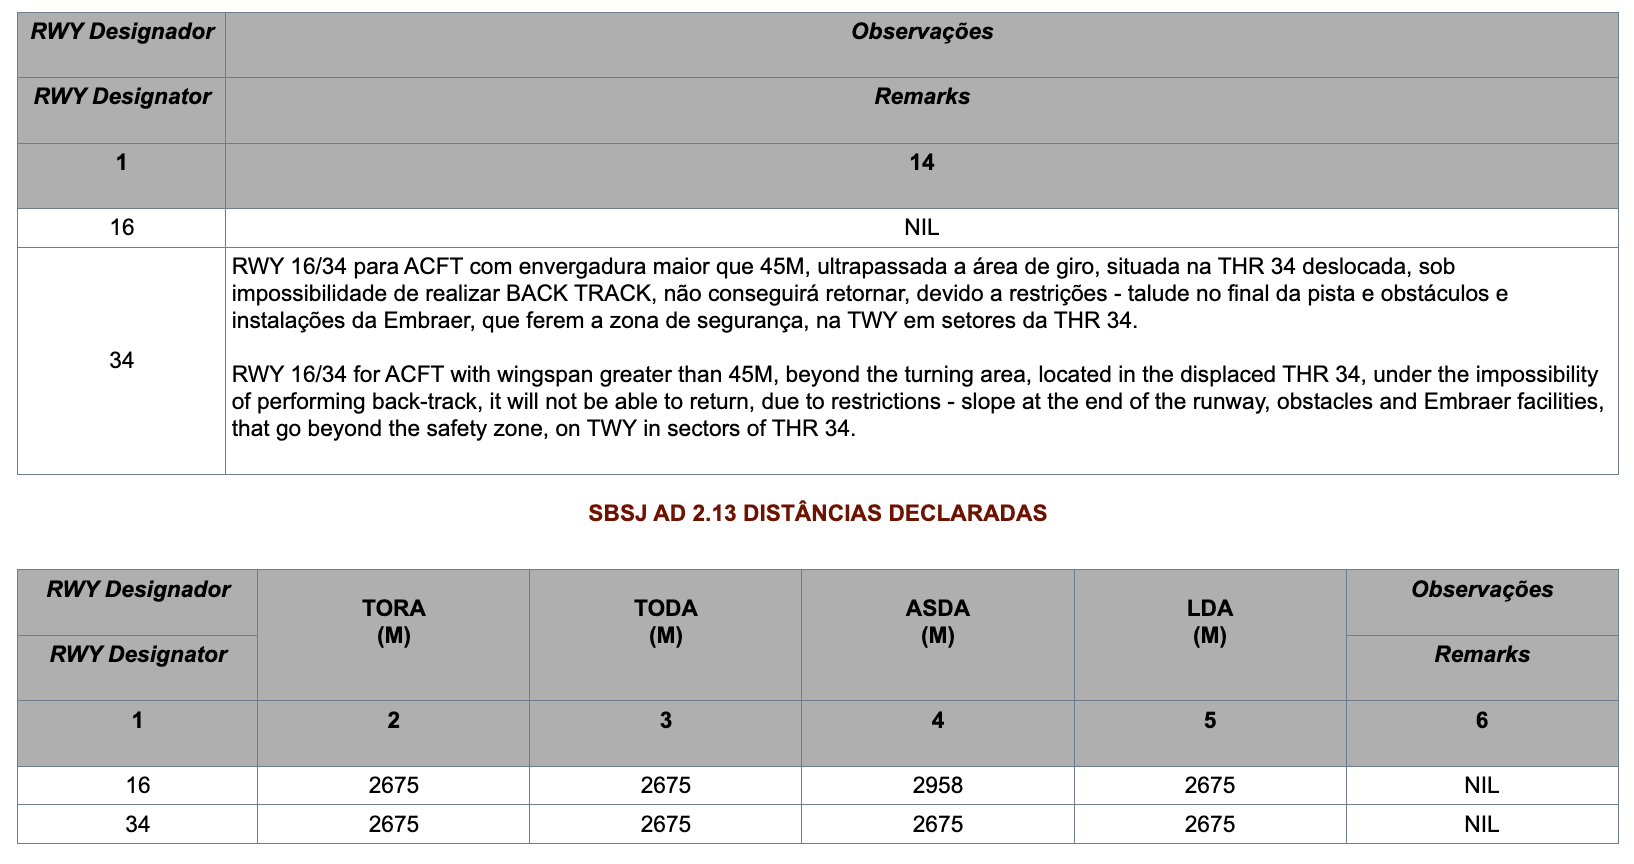
\includegraphics[width=\linewidth]{Figures/aip212.png}
    \caption{Observações da seção AD~2.12 e distâncias declaradas da seção AD~2.13 da AIP do SBSJ.}
    \label{fig:aip-ad212}
    \par\smallskip{\small Fonte: \citeonline{decea2026aip}.}
\end{figure}

\subsection{R5: posição relativa}\label{sec:req-posicao}

As posições devem ser registradas em relação a pontos efetivamente medidos, e não por coordenadas próprias. Uma nova medição de um desses pontos deve, então, propagar-se a todas as posições que dependem dele, sem que nenhuma delas precise ser reescrita. É a propriedade do referenciamento linear (Seção~\ref{sec:iso19148}) aplicada ao lado ar.

\subsection{R6: estrutura comum e conteúdo flexível}\label{sec:req-forma}

Todos os elementos devem compartilhar uma forma mínima, e o restante do conteúdo deve ser livre. A forma mínima é o que permite tratar qualquer elemento da mesma maneira, isto é, a sua identidade, o seu tipo, a sua posição ou relação com outros elementos e as premissas de que dependem os valores derivados. O conteúdo livre acomoda a diversidade entre aeródromos, que nenhum esquema fixo antecipa. Uma informação ausente deve, além disso, distinguir-se de uma informação nula.

\subsection{R7: verificação por terceiro}\label{sec:req-verificacao}

Quem recebe os dados deve poder conferir a sua integridade sem confiar em quem os publica, nem no código de quem os publica. Para isso, a forma de verificação precisa ser pública e simples o bastante para ser reimplementada de forma independente.

\section{Estudo de caso e dados}\label{sec:caso}

O estudo de caso é a pista 16/34 do Aeroporto de São José dos Campos (SBSJ). A escolha se deve a dois fatores. O primeiro é a existência de duas cartas oficiais, de 2022 e de 2026, com valores diferentes para a mesma pista (Figura~\ref{fig:adc-aoc}), o que permite caracterizar a lacuna com dados reais. O segundo é a configuração simples, com uma única pista, que isola as propriedades avaliadas de questões de composição entre vários elementos.

Os dados vêm de três publicações do DECEA:
\begin{itemize}
    \item a AIP, seções AD~2.12 e AD~2.13, com as coordenadas, as elevações e a ondulação geoidal das cabeceiras, a largura da pista, as dimensões da zona de parada e as distâncias declaradas \cite{decea2026aip};
    \item a Carta de Obstáculos de Aeródromo, emenda AIRAC~2213 \cite{decea2022aoc};
    \item a Carta de Aeródromo, emenda AIRAC~2604 \cite{decea2026adc}.
\end{itemize}

Apenas as premissas entram no registro. Os valores que a AIP publica e que podem ser calculados, como o comprimento, os azimutes e as distâncias declaradas, ficam de fora e servem de gabarito. As duas cartas servem apenas ao contraste do E1. A remedição da cabeceira~34 e as restrições temporárias são simuladas, pois não ocorreram no período estudado, e servem para exercitar o ciclo de vida dos elementos.

\section{Experimentos}\label{sec:experimentos}

São seis experimentos, cada um dedicado a uma propriedade da hipótese. O E1 é um contraste. Ele registra os dados na forma em que as publicações chegam ao usuário e verifica o que esse registro permite responder. Os demais usam a arquitetura proposta. A Tabela~\ref{tab:experimentos} apresenta as perguntas e os critérios de aprovação, e a Seção~\ref{sec:procedimentos} descreve como cada experimento é executado.

\begin{table}[htbp]
    \centering
    \caption{Perguntas e critérios de aprovação dos experimentos.}
    \label{tab:experimentos}
    \small
    \begin{tabularx}{\linewidth}{l X X}
        \toprule
        & Pergunta & Critério de aprovação \\
        \midrule
        E1 & O modelo que guarda o valor publicado registra a causa das mudanças entre edições? & contraste: nenhum campo alterado traz causa \\
        E2 & Os valores derivados reproduzem os publicados? A remedição de uma cabeceira obriga a reescrever outro dado? & diferença dentro da margem de cada grandeza; a remedição grava apenas o levantamento e a troca de referencial; diferença ao gabarito geodésico abaixo de 0,5~mm \\
        E3 & O estado em qualquer instante é reconstruído, com autor, motivo e causa de cada mudança? & estados esperados em todos os instantes consultados; derivados de um instante passado idênticos antes e depois da remedição \\
        E4 & Quais alterações feitas diretamente no banco são detectadas, e por qual mecanismo? & alterar, apagar e inserir eventos detectados pela cadeia; reescrita completa detectada pela âncora \\
        E5 & Produtos gerados do mesmo registro divergem? Um terceiro verifica o registro sem a biblioteca? & mesmos valores nos dois produtos; o verificador independente chega à mesma cabeça e aponta o evento alterado \\
        E6 & A leitura pelo tópico equivale à do banco, sem estados intermediários e com o canal adulterado percebido? & mesmas respostas em todos os cortes; nenhum corte dentro de um grupo; recorte com os mesmos derivados; recusa da leitura além do recebido; mesmo \textit{hash} nos seis consumidores; adulteração no meio do tópico interrompe o consumo \\
        \bottomrule
    \end{tabularx}
    \par\smallskip{\small Fonte: o autor.}
\end{table}
% CONFERIR: citar os commits em que as verificações foram registradas antes da execução.

Nenhuma margem foi escolhida livremente. As margens das grandezas publicadas decorrem da precisão com que a AIP publica cada valor e as coordenadas de que ele depende, definida no PANS-AIM \cite{icao2018pansaim}. O comprimento, por exemplo, é publicado ao metro, e as coordenadas das cabeceiras, a 0,01\textquotedbl. O valor calculado pode, então, diferir do publicado em até 0,919~m, sendo 0,5~m do arredondamento ao metro e 0,419~m do efeito do arredondamento das coordenadas. Pelo mesmo raciocínio, resultam $\pm$1,419~m para a ASDA~16, que soma o arredondamento da zona de parada, $\pm$0,014$^\circ$ para os azimutes e $\pm$1,009$^\circ$ para os rumos magnéticos, publicados em graus inteiros, assim como a variação magnética. O Apêndice~\ref{ape:testes} lista as verificações de cada experimento. A comparação com o gabarito geodésico usa a exatidão de 0,5~mm das fórmulas de Vincenty (Seção~\ref{sec:geodesia}). As verificações foram registradas no histórico do repositório de experimentos antes da sua execução \cite{aeroledger_experimentos}.

\section{Verificação interna e comparação externa}\label{sec:validacao}

Uma biblioteca que confere o que ela própria gravou mostra consistência por construção, e não correção. Por isso, a avaliação distingue dois tipos de verificação. A verificação interna confere que a biblioteca devolve o que gravou e que as suas regras são cumpridas. A comparação externa confronta os resultados com referências que não dependem da biblioteca.

Três referências externas são usadas. A primeira são os valores da AIP que não entram no modelo, como o comprimento, os azimutes e as distâncias declaradas, que a arquitetura precisa recalcular. A segunda é um gabarito geodésico, uma implementação das fórmulas de Vincenty escrita separadamente e validada em um caso publicado. A terceira é um verificador independente, escrito apenas a partir da especificação pública da cadeia, sem o código da biblioteca.

\section{Reprodutibilidade}\label{sec:reprodutibilidade}

Os experimentos usam a biblioteca \texttt{aeroledger}, versão 0.6.0 (\textit{commit} \texttt{e93b718}) \cite{aeroledger}, e são executados por um \textit{notebook} mantido em repositório separado \cite{aeroledger_experimentos}. A separação garante que a biblioteca avaliada não contenha código escrito para o experimento. O banco extraído do SBSJ, gerado a partir do mesmo cenário, está publicado como conjunto de dados aberto \cite{aeroledger_dataset} e permite repetir parte da avaliação sem a biblioteca (Seção~\ref{sec:res-banco}).


\chapter{Desenvolvimento e aplicação}\label{chap:solucao}
O Capítulo~\ref{chap:metodologia} estabeleceu os requisitos que um serviço de dados auditável deve atender e o método pelo qual a solução é avaliada. Este capítulo desenvolve a solução e a aplica ao caso estudado.

As Seções~\ref{sec:visao-geral} a~\ref{sec:banco-extraido} descrevem a arquitetura seguindo o caminho do dado. Primeiro, apresentam o que se guarda, isto é, o evento, o tempo e o referencial. Em seguida, mostram como se escreve e como se lê, como a leitura chega aos consumidores, como um terceiro confere o que recebeu e como o registro é entregue em um arquivo. A Seção~\ref{sec:implementacao} descreve a implementação, e a Seção~\ref{sec:aplicacao-sbsj}, a sua aplicação à pista do SBSJ. As Seções~\ref{sec:extensoes} e~\ref{sec:limites-arq} reúnem, respectivamente, o que foi desenhado sem ser avaliado e os limites conhecidos da arquitetura.

\section{Visão geral}\label{sec:visao-geral}

A arquitetura parte de uma ideia central. O dado primário não é o estado do aeródromo, mas a sequência de afirmações feitas sobre ele, e o estado em qualquer instante é calculado a partir dessa sequência. Essa organização corresponde ao padrão \textit{event sourcing} (Seção~\ref{sec:event-sourcing}), onde cada alteração é gravada como um evento, e os eventos nunca são alterados. O estado, então, resulta da composição dos eventos até o instante pedido.

A essa ideia soma-se a separação entre escrita e leitura (CQRS). Do lado da escrita, um único ponto de entrada valida e grava os eventos, e o que ele grava é a única fonte de verdade. Do lado da leitura, cada produto é um modelo de leitura montado a partir dos mesmos eventos, como, por exemplo, o conteúdo de uma carta ou uma tabela de distâncias declaradas. Os modelos de leitura podem ser vários, podem mudar e podem ser apagados e reconstruídos, pois não guardam nada que não esteja nos eventos.

A arquitetura tem quatro peças, apresentadas na Tabela~\ref{tab:pecas}, e cada requisito da Seção~\ref{sec:requisitos} é atendido por um mecanismo dessas peças, como resume a Tabela~\ref{tab:requisitos-mecanismos}.

\begin{table}[htbp]
    \centering
    \caption{As quatro peças da arquitetura e o seu papel em CQRS.}
    \label{tab:pecas}
    \begin{tabularx}{\linewidth}{l l X}
        \toprule
        Peça & Papel & Função \\
        \midrule
        Registro & Comandos e registro de eventos & Recebe a escrita, valida a forma e grava os eventos encadeados por \textit{hash} \\
        Tópico geral & Publicação dos eventos & Publica o registro, em ordem, fora do banco \\
        Consumidores & Modelos de leitura & Conferem a cadeia, guardam o que leram e respondem com limite explícito \\
        Banco extraído & Cópia portátil do registro & Entrega, em um arquivo, os mesmos eventos e \textit{hashes}, com visões de leitura \\
        \bottomrule
    \end{tabularx}
    \par\smallskip{\small Fonte: o autor.}
\end{table}

\begin{table}[htbp]
    \centering
    \caption{Requisitos do artefato e os mecanismos que os atendem.}
    \label{tab:requisitos-mecanismos}
    \begin{tabularx}{\linewidth}{l X l}
        \toprule
        Requisito & Mecanismo & Seção \\
        \midrule
        R1 Origem de cada valor & Autor, motivo e causa no envelope de cada evento & \ref{sec:registro} \\
        R2 Reconstrução no tempo & Registro em que só se acrescenta; tempo de transação como única linha do tempo & \ref{sec:registro}, \ref{sec:tempo} \\
        R3 Consistência entre produtos & Produtos como modelos de leitura da mesma fonte, com limite explícito e regra identificada & \ref{sec:leitura}, \ref{sec:distribuicao} \\
        R4 Mínimo de informação & Derivados calculados na leitura, gravados só se necessário& \ref{sec:leitura} \\
        R5 Posição relativa & Referencial com referentes e posições $(e, r, s, o, v)$ & \ref{sec:referencial} \\
        R6 Estrutura comum e conteúdo flexível & Envelope fixo e corpo sem esquema, achatado em linhas & \ref{sec:registro} \\
        R7 Verificação por terceiros & Cadeia de \textit{hash} sobre forma canônica pública, conferida na leitura e no arquivo & \ref{sec:escrita}, \ref{sec:verificacao} \\
        \bottomrule
    \end{tabularx}
    \par\smallskip{\small Fonte: o autor.}
\end{table}

A arquitetura não depende de um banco de eventos ou de grafos dedicado, por exemplo, um banco relacional comum é suficiente. A escolha é deliberada, pois as propriedades decorrem da forma como os dados são escritos e lidos. O banco extraído (Seção~\ref{sec:banco-extraido}) é a demonstração mais direta disso, já que as mesmas propriedades valem em um arquivo, sem servidor.

A Tabela~\ref{tab:origem} indica a origem de cada elemento da arquitetura. Um elemento \emph{adotado} é usado como descrito na sua fonte, e a contribuição está apenas na sua aplicação ao domínio. Um elemento \emph{adaptado} parte de uma base conhecida, modificada para atender aos requisitos do Capítulo~\ref{chap:metodologia}, e a modificação é descrita na última coluna. Um elemento \emph{proposto} não tem precedente direto na literatura revisada, e a coluna de base indica, quando existe, o precedente mais próximo. A contribuição do trabalho concentra-se nos elementos adaptados e propostos, o que a caracteriza como exaptação, no sentido de \citeonline{gregor2013}.

\begin{table}[htbp]
    \centering
    \caption{Origem dos elementos da arquitetura.}
    \label{tab:origem}
    \small
    \begin{tabularx}{\linewidth}{X X X}
        \toprule
        Elemento & Base & Situação neste trabalho \\
        \midrule
        Registro em que só se acrescenta; estado derivado dos eventos & \textit{event sourcing} \cite{fowler2005,kleppmann2017} & adotado \\
        Separação entre escrita e leitura & CQRS \cite{young2010} & adotado \\
        Correção por novo lançamento & livro-razão \cite{helland2016} & adotado \\
        Encadeamento por \textit{hash} sobre forma canônica & \citeonline{haber1991}; RFC~8785 & adotado \\
        Ciclo de vida \texttt{BASELINE}, \texttt{DELTA} e \texttt{VOID} & \textit{TimeSlices} do AIXM & adaptado: o temporário é o ciclo de vida de uma \textit{feature} própria \\
        Posições por referente & ISO~19148 & adaptado: duas pontas medidas; azimute e declividade nunca registrados \\
        Grupos atômicos & partidas dobradas & adaptado: sem lei de conservação, a atomicidade é imposta na escrita \\
        Consumidores sobre canal não confiável & registro ordenado e CDC \cite{kleppmann2017} & adaptado: conferência da cadeia, limite explícito e fecho de dependência \\
        Referencial endereçado pelo conteúdo e trocado por evento & endereçamento por conteúdo \cite{merkle1988} & adaptado: o referencial do referenciamento linear é um objeto imutável, e a remedição é a troca de referencial por evento \\
        Distâncias declaradas derivadas na leitura, com regra identificada & regras do Anexo~14; dados derivados \cite{kleppmann2017} & proposto \\
        Banco extraído como extrato verificável & extrato do livro-razão; resumos do SQL Ledger \cite{antonopoulos2021} & proposto \\
        \bottomrule
    \end{tabularx}
    \par\smallskip{\small Fonte: o autor.}
\end{table}

\section{O registro}\label{sec:registro}

\subsection{\textit{Features}, envelope e corpo}

Cada elemento do lado ar é uma \textit{feature}, no sentido do AIXM (Seção~\ref{sec:aixm}). São \textit{features} uma pista, uma cabeceira, uma zona de parada, uma restrição, um levantamento topográfico, o próprio aeródromo e, também, os eventos operacionais. Toda alteração de uma \textit{feature} é um evento, composto por um envelope e um corpo.

O envelope identifica o evento e indica a sua origem. Ele tem a mesma forma para todos os tipos de \textit{feature}, e é nele que se atende ao requisito de origem de cada valor (Seção~\ref{sec:req-origem}). Os seus campos são os seguintes:
\begin{itemize}
    \item \texttt{feature\_id} e \texttt{feature\_type} identificam a \textit{feature} e o seu tipo, como \texttt{airport}, \texttt{runway}, \texttt{runway\_direction}, \texttt{protect\_area}, \texttt{restriction} e \texttt{survey};
    \item \texttt{event\_type} indica o papel do evento no ciclo de vida da \textit{feature} (Seção~\ref{sec:ciclo-vida});
    \item \texttt{asserted\_by} registra quem afirma, e é obrigatório e não vazio;
    \item \texttt{reason} registra o motivo, e é obrigatório no encerramento;
    \item \texttt{caused\_by} aponta o evento que motivou este, quando houver;
    \item \texttt{owner\_ref} aponta a \textit{feature} a que esta pertence, quando houver;
    \item \texttt{grupo\_id} e \texttt{grupo\_n} aparecem somente quando o evento integra uma mudança composta por vários eventos (Seção~\ref{sec:grupos}).
\end{itemize}
\begin{figure}[htbp]
    \centering
    \begin{subfigure}{\linewidth}
        \centering
        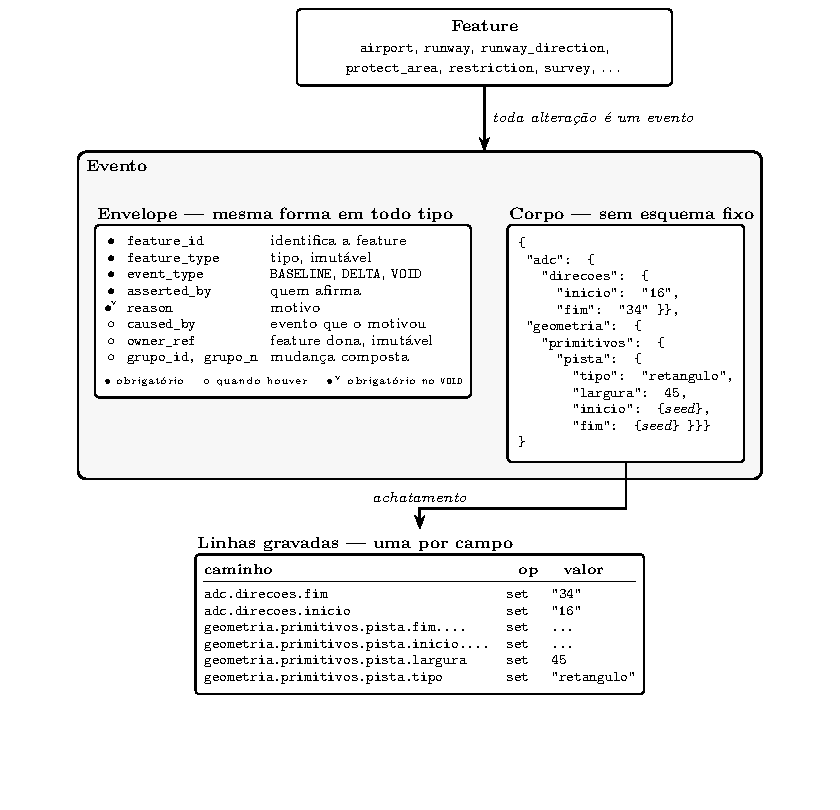
\includegraphics[page=1]{Figures/fig_evento_envelope_corpo.pdf}
        \caption{Envelope, corpo e as linhas gravadas a partir do corpo.}
        \label{fig:evento-estrutura}
    \end{subfigure}

    \bigskip
    \begin{subfigure}{\linewidth}
        \centering
        \includegraphics[page=2]{Figures/fig_evento_envelope_corpo.pdf}
        \caption{Grafo de causas, com exemplos ilustrativos.}
        \label{fig:evento-causas}
    \end{subfigure}

    \caption{Estrutura de um evento e encadeamento das causas.}
    \label{fig:evento}
    \par\smallskip{\small Fonte: o autor.}
\end{figure}
A causa só pode apontar para um evento já existente no mesmo registro e anterior ao que a declara. Por isso, as causas formam um grafo acíclico, e toda cadeia de causas termina em um evento sem causa anterior. Esse evento é uma observação, como o levantamento de uma cabeceira, ou uma decisão, como a publicação inicial de uma pista. O tipo e o dono de uma \textit{feature} também não mudam ao longo da sua vida, de modo que uma pista não se converte em pista de táxi. Uma reclassificação desse tipo é registrada como o encerramento de uma \textit{feature} seguido da criação de outra.

O corpo contém o que se afirma sobre a \textit{feature}. Ele não tem esquema fixo e consiste em um documento JSON organizado em camadas, como a camada física, com a qualidade do pavimento, e a camada de geometria, com as posições. Na gravação, o corpo é achatado em linhas, uma por campo. Cada linha é identificada pelo caminho do campo, de forma análoga ao acesso às propriedades de um objeto (por exemplo, \texttt{geometria.primitivos.pista.largura}), e registra a operação, de definição ou de remoção, e o novo valor. Esse achatamento atende ao requisito de estrutura comum e conteúdo flexível (Seção~\ref{sec:req-forma}), e dele decorrem três propriedades:
\begin{itemize}
    \item a leitura pode restringir-se a uma camada, pois um índice por caminho permite ler apenas a geometria de uma pista, sem abrir o restante do corpo;
    \item um campo ausente distingue-se de um campo nulo, já que o primeiro não foi informado e o segundo foi informado como vazio;
    \item um evento de alteração grava apenas os campos que mudam, e a diferença entre dois instantes é a lista desses campos, com os valores anteriores e posteriores.
\end{itemize}

\subsection{Ciclo de vida}\label{sec:ciclo-vida}

Há três tipos de evento, com nomes emprestados do AIXM:
\begin{itemize}
    \item \texttt{BASELINE} cria a \textit{feature} com o corpo completo, ou a recria após um encerramento;
    \item \texttt{DELTA} altera campos do corpo e grava apenas os caminhos alterados, sem repetir o estado anterior, que já está nos eventos precedentes;
    \item \texttt{VOID} encerra o ciclo de vida da \textit{feature} e exige um motivo. Não se trata de exclusão nem de anulação de um evento anterior; o histórico permanece, e a \textit{feature} apenas deixa de existir a partir daquele instante.
\end{itemize}

O significado desses tipos é mais simples que no AIXM, pois não há distinção estrutural entre alteração permanente e temporária. Uma interdição temporária, por exemplo, é uma \textit{feature} de restrição, com a pista como dona, criada por um \texttt{BASELINE} e encerrada por um \texttt{VOID}, e a sua duração resulta da sequência de eventos. Operações como substituir, dividir ou fundir \textit{features} também não são primitivas, e se compõem de sequências de \texttt{BASELINE} e \texttt{VOID}. A Figura~\ref{fig:ciclo-vida} mostra os estados de uma \textit{feature} e as transições que a escrita recusa.

\begin{figure}[htbp]
    \centering
    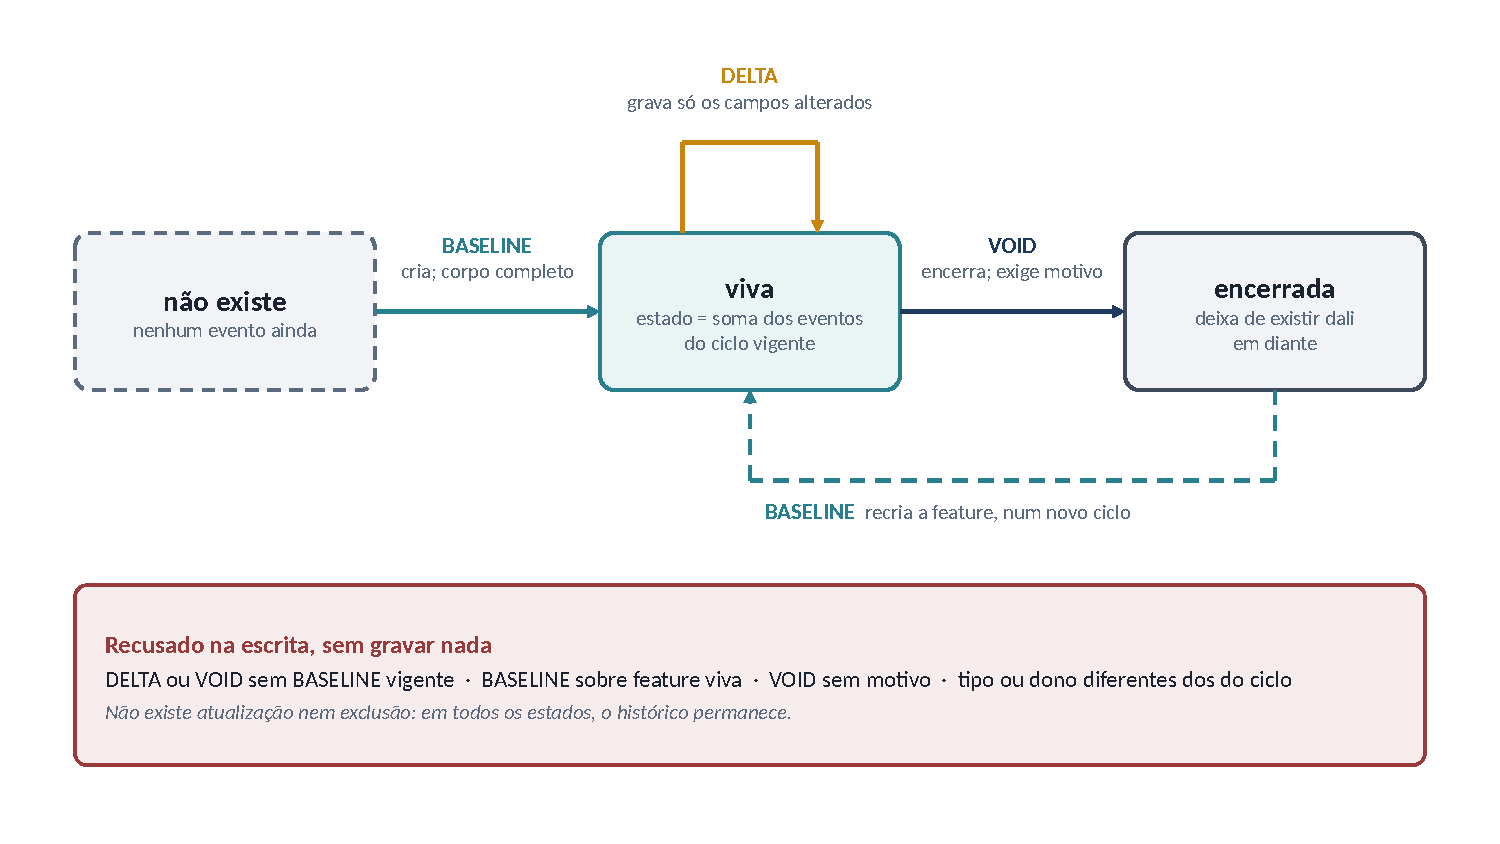
\includegraphics[width=\linewidth]{Figures/fig_ciclo_vida.pdf}
    \caption{Ciclo de vida de uma \textit{feature} e as transições que a escrita recusa.}
    \label{fig:ciclo-vida}
    \par\smallskip{\small Fonte: o autor.}
\end{figure}


\subsection{Grupos}\label{sec:grupos}

Algumas mudanças exigem mais de um evento. A carga de uma edição do AIP, por exemplo, cria de uma só vez o aeródromo, a pista, as cabeceiras e a zona de parada. Uma leitura feita no meio dessa carga mostraria a pista sem a zona de parada e calcularia uma ASDA igual à TORA, sem nenhum erro aparente. Para evitar esse estado intermediário, a arquitetura define o grupo, um conjunto de dois ou mais eventos gravados juntos, ou todos ou nenhum, contíguos no registro e no mesmo instante.

Cada evento do grupo leva no envelope o \texttt{grupo\_id}, que é o identificador do primeiro evento, e o \texttt{grupo\_n}, que é o número de eventos do grupo. O primeiro campo registra quais eventos formam uma mesma mudança, o que o instante comum, por si só, não garante. O segundo permite a quem lê saber se já recebeu o grupo inteiro. Uma leitura cujo limite caia dentro de um grupo recua até antes dele, de modo que nenhum corte mostra uma mudança pela metade (Seção~\ref{sec:distribuicao}).

O grupo cumpre o papel do lançamento em um livro-razão de partidas dobradas, no qual as partidas de uma transferência entram juntas e o livro nunca mostra o débito sem o crédito. Há, contudo, uma diferença. Na contabilidade, as partidas de um lançamento somam zero, e uma transferência incompleta se denuncia sozinha. Aqui não há lei de conservação, e uma pista sem zona de parada é um estado plausível. A atomicidade, por isso, não pode depender de uma conferência posterior.

\section{Tempo}\label{sec:tempo}

A arquitetura usa uma única linha do tempo, o tempo de transação, isto é, o instante em que cada evento foi registrado (Seção~\ref{sec:bitemporal}). Os motivos dessa escolha estão na Seção~\ref{sec:req-tempo}. Cada aeródromo tem a sua cadeia de eventos, e cada cadeia tem um relógio que só avança, de modo que nada se escreve no passado. A Figura~\ref{fig:linha-tempo} ilustra a linha do tempo de duas \textit{features}.

\begin{figure}[h]
    \centering
    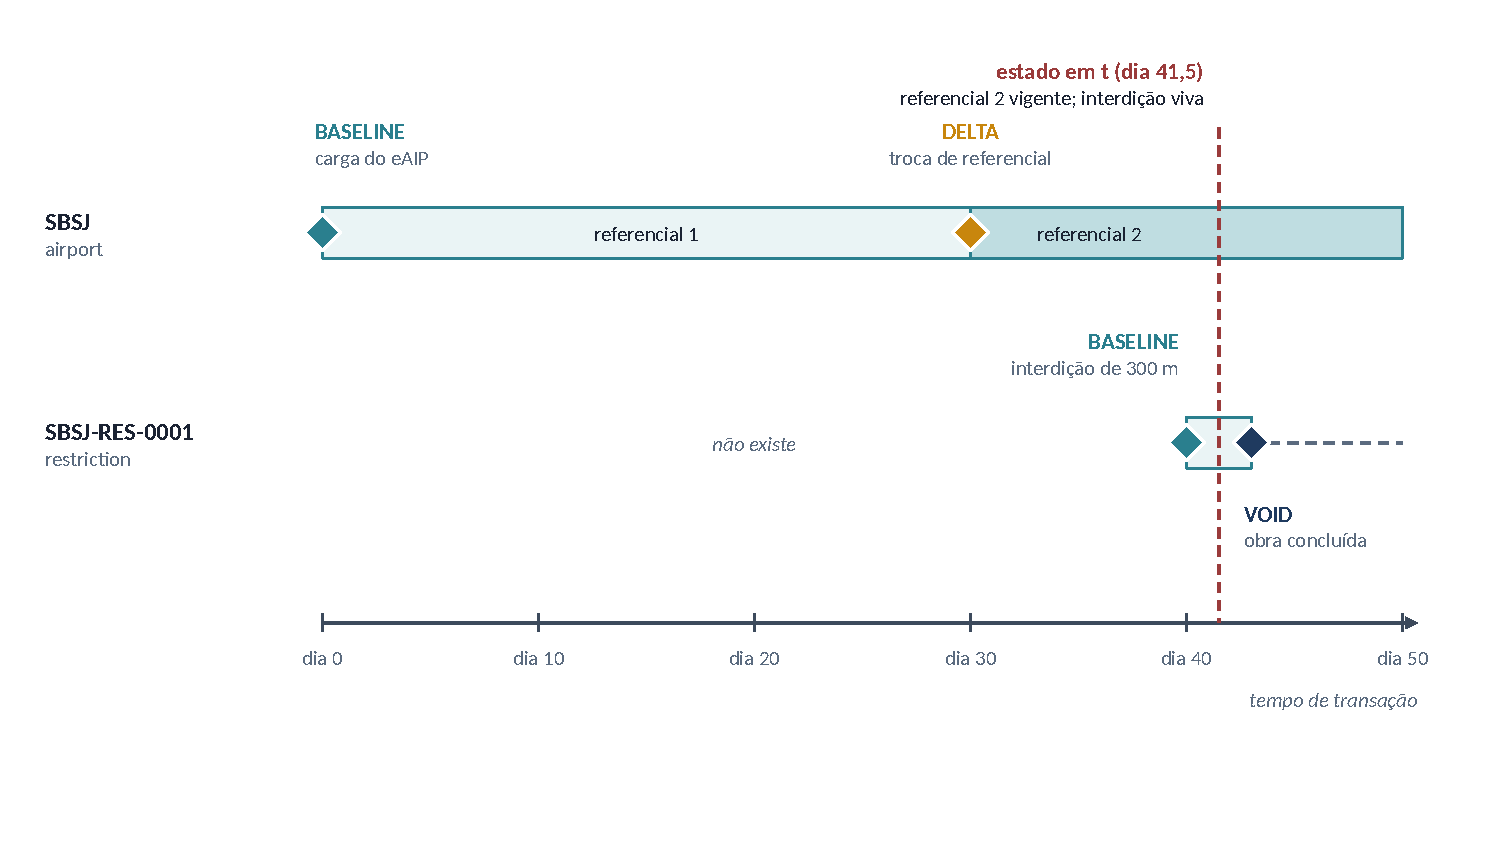
\includegraphics[width=\linewidth]{Figures/fig_ciclo_vida_tempo.pdf}
    \caption{Linha do tempo de duas \textit{features} e o estado em um instante $t$.}
    \label{fig:linha-tempo}
    \par\smallskip{\small Fonte: o autor.}
\end{figure}


O identificador do evento (\texttt{event\_id}) segue o esquema Snowflake \cite{twitter2010snowflake}, com 41 \textit{bits} de milissegundos desde uma data arbitrária, 10 de partição e 12 de sequência (Figura~\ref{fig:snowflakeid}). O instante é extraído do próprio identificador, cuja ordem coincide com a do tempo, e a escrita recusa um evento anterior ao último gravado.

\begin{figure}[htbp]
    \centering
    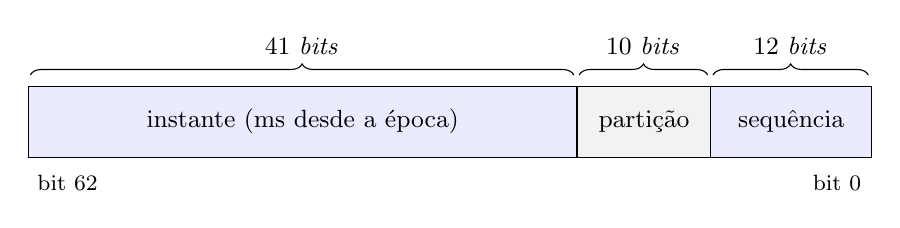
\begin{tikzpicture}[x=0.17cm, y=1cm, font=\small,
        campo/.style={draw, minimum height=0.9cm, anchor=south west, inner sep=0pt}]
        % larguras proporcionais ao número de bits: 41 | 10 | 12
        \node[campo, fill=blue!8,  minimum width=41*0.17cm] at (0,0)  {instante (ms desde a época)};
        \node[campo, fill=gray!10, minimum width=10*0.17cm] at (41,0) {partição};
        \node[campo, fill=blue!8,  minimum width=12*0.17cm] at (51,0) {sequência};
        \foreach \a/\b/\n in {0/41/41, 41/51/10, 51/63/12} {
            \draw[decorate, decoration={brace, amplitude=4pt}] (\a+0.2,1.05) -- (\b-0.2,1.05)
                node[midway, above=4pt] {\n\ \textit{bits}};
        }
        \node[anchor=north west, font=\footnotesize] at (0,-0.1) {bit 62};
        \node[anchor=north east, font=\footnotesize] at (63,-0.1) {bit 0};
    \end{tikzpicture}
    \caption{Composição do identificador de um evento.}
    \label{fig:snowflakeid}
    \par\smallskip{\small Fonte: o autor.}
\end{figure}

Na leitura, o instante $t$ pode ser uma data e hora ou um \texttt{event\_id}, e ambos são convertidos em um limite superior de identificador. Uma data e hora corresponde ao maior identificador possível naquele milissegundo, e um \texttt{event\_id} distingue eventos do mesmo milissegundo, como os de um grupo. Toda consulta se reduz, assim, a ``tudo até o evento $N$''.

A extensão para dois eixos de tempo está entre as propostas da Seção~\ref{sec:extensoes}, no qual uma data alegada por quem escreve, como a data de uma medição ou a entrada em vigor de uma emenda AIRAC, é conteúdo do corpo. 

\section{Referencial e posição}\label{sec:referencial}

\subsection{O referencial}

O requisito de posição relativa (Seção~\ref{sec:req-posicao}) é atendido por um referencial, documento que declara os referentes, isto é, os pontos medidos em que as posições se apoiam, e os elementos lineares entre eles. No SBSJ, o referencial tem dois referentes georreferenciados, as cabeceiras THR16 e THR34, e um elemento linear entre elas, RWY\_16\_34. Cada referente tem latitude, longitude, elevação, ondulação geoidal e fonte, e o datum é o SIRGAS2000. A Figura~\ref{fig:referencial-sbsj} mostra esse referencial.

\begin{figure}[htbp]
    \centering
    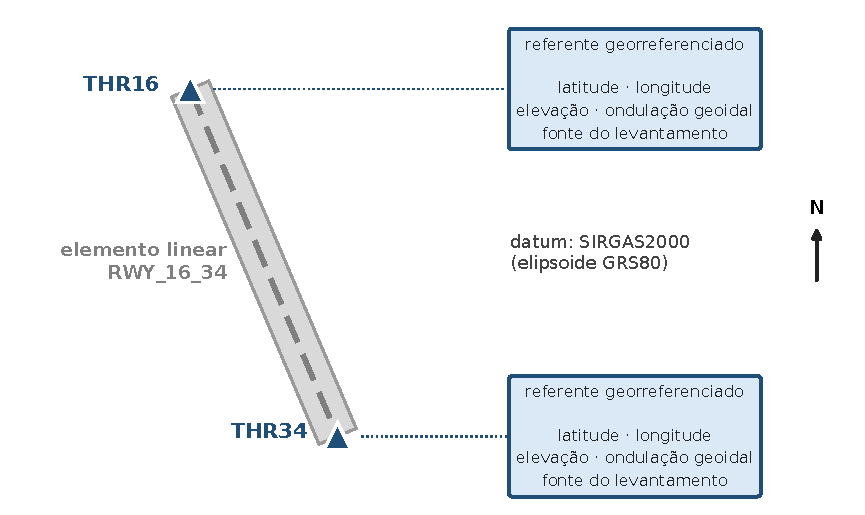
\includegraphics[width=0.85\linewidth]{Figures/fig-referencial-sbsj.pdf}
    \caption{Referencial do SBSJ: as cabeceiras THR16 e THR34 como referentes georreferenciados e o elemento linear RWY\_16\_34 entre elas.}
    \label{fig:referencial-sbsj}
    \par\smallskip{\small Fonte: o autor.}
\end{figure}

A publicação de um referencial deve seguir as seguintes regras (Figura~\ref{fig:regras-referencial}), sob pena de ser rejeitada:
\begin{itemize}
    \item cada referente deve ser definido por exatamente um dos seguintes
    métodos: por georreferenciamento, com latitude e longitude, ou por
    posicionamento relativo a outro referente, medido ao longo de um
    elemento linear a partir de uma de suas pontas;
    \item as relações entre referentes não podem formar ciclos, e todo
    encadeamento deve terminar em um referente georreferenciado;
    \item todo elemento linear deve possuir exatamente duas pontas distintas;
    \item o posicionamento relativo de um referente exige um elemento linear,
    pois, sem ele, não há uma direção definida para determinar o afastamento
    em relação ao referente de origem.
\end{itemize}

\begin{figure}[htbp]
    \centering
    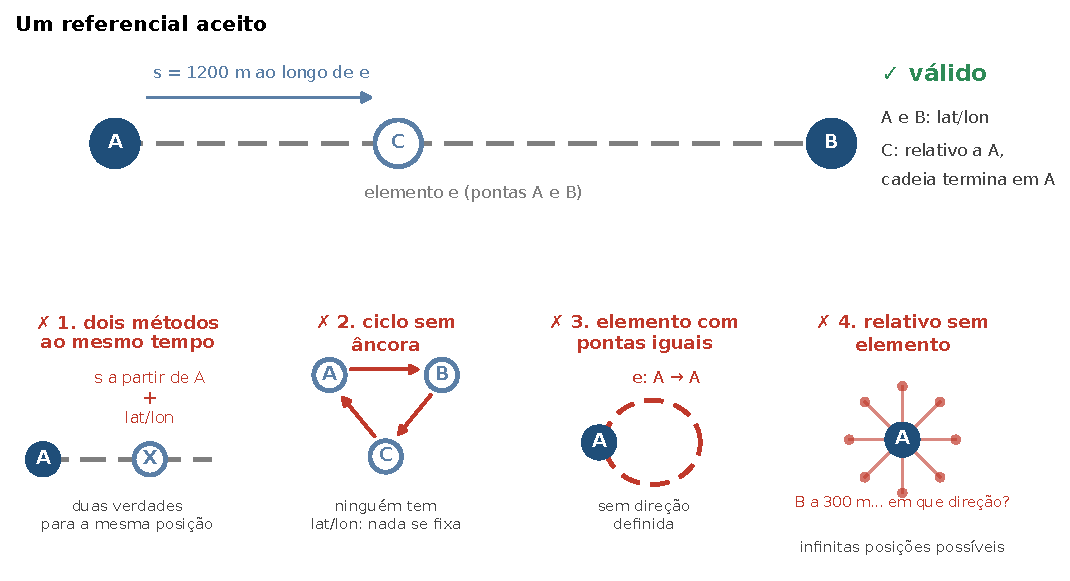
\includegraphics[width=\linewidth]{Figures/fig-regras-referencial.pdf}
    \caption{Exemplo de referencial aceito e um caso de rejeição para cada regra de publicação.}
    \label{fig:regras-referencial}
    \par\smallskip{\small Fonte: o autor.}
\end{figure}

O número de referentes é livre. Um aeroporto com várias pistas teria um elemento linear por eixo, e os referentes de uma pista poderiam ser independentes dos de outra. Essa configuração não é avaliada neste trabalho.

O referencial é endereçado pelo conteúdo, ou seja, o seu identificador (\texttt{ref\_id}) é o \textit{hash} SHA-256 da sua forma canônica (Seção~\ref{sec:escrita}). Dois referenciais com o mesmo conteúdo têm o mesmo identificador, e nenhum pode ser alterado sem mudar de identificador. O referencial vigente é um campo do corpo da \textit{feature} \texttt{airport}, e trocá-lo é um \texttt{DELTA} nessa \textit{feature}. A escrita recusa a troca se alguma posição gravada ficar sem apoio no novo referencial.

\subsection{Posições}

Toda posição que não seja um referente é gravada como uma \textit{seed}, segundo o referenciamento linear da ISO~19148 (Equação~\ref{eq:lrs}). O elemento linear $e$ fornece a direção, e o referente $r$, sempre sobre o elemento, fornece a origem. A distância $s$ é positiva no sentido da outra ponta do elemento, e o afastamento lateral $o$ é positivo à direita de quem percorre o elemento no sentido de $s$. A altitude da posição é
\begin{equation}
    z(p) = z_r + v
    \label{eq:altitude-posicao}
\end{equation}
em que $z_r$ é a altitude do referente e $v$ o afastamento vertical. Os componentes da \textit{seed} estão ilustrados na Figura~\ref{fig:seed-lrs}.

\begin{figure}[htbp]
    \centering
    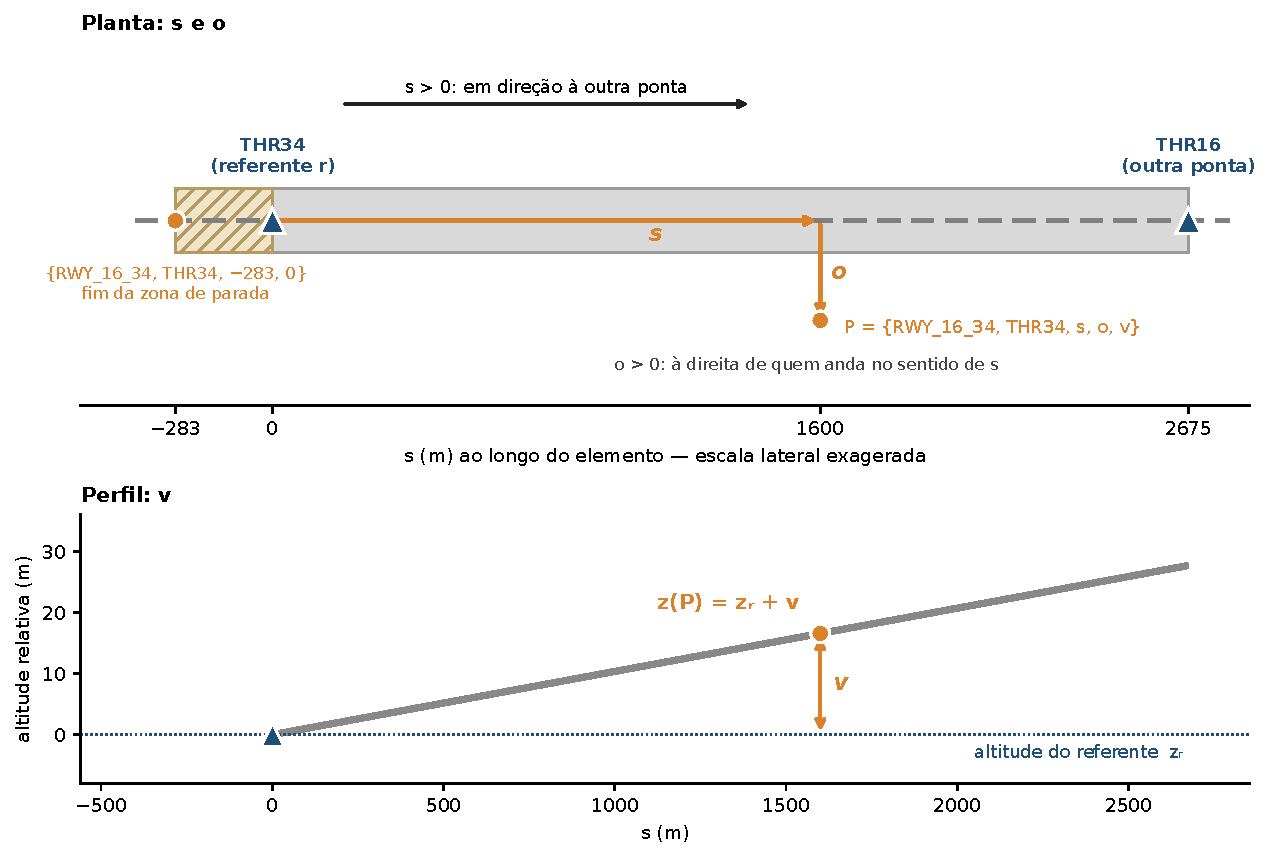
\includegraphics[width=\linewidth]{Figures/fig-seed-lrs.pdf}
    \caption{Componentes de uma \textit{seed}: em planta, a distância $s$ e o afastamento lateral $o$; em perfil, o afastamento vertical $v$ a partir da altitude do referente. A escala lateral da planta está exagerada.}
    \label{fig:seed-lrs}
    \par\smallskip{\small Fonte: o autor.}
\end{figure}

A zona de parada do SBSJ, por exemplo, termina em $\{\mathrm{RWY\_16\_34},\, \mathrm{THR34},\, -283,\, 0\}$, isto é, 283~m para fora da cabeceira~34, sobre o eixo. Um afastamento vertical ausente significa ``não informado'', e não zero. A posição continua definida no plano, mas a sua altitude não. Em uma pista em rampa, um zero implícito atribuiria à posição a altitude do referente, o que estaria errado. A Figura~\ref{fig:afastamento-vertical-ausente} ilustra a diferença.

\begin{figure}[htbp]
    \centering
    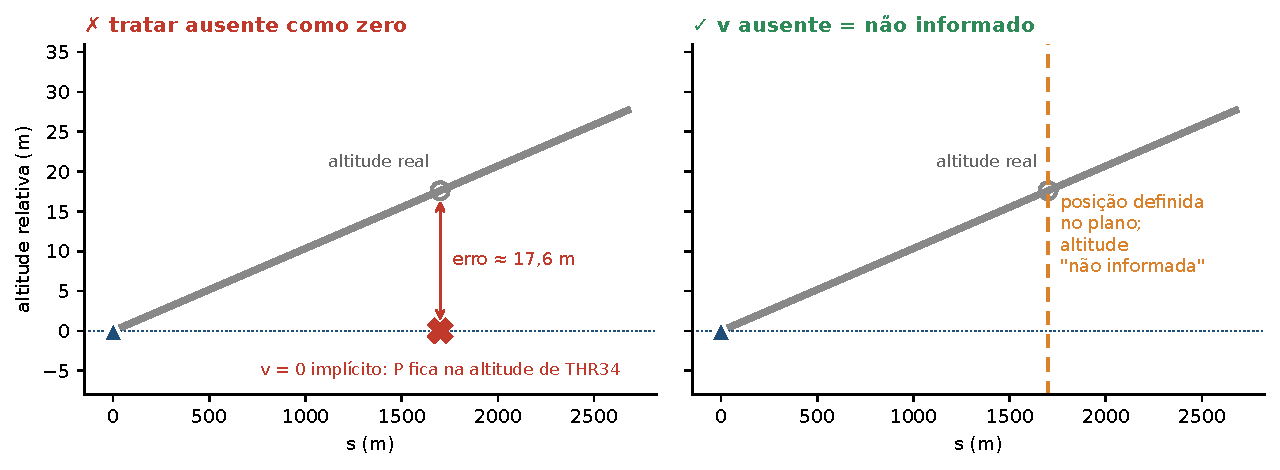
\includegraphics[width=\linewidth]{Figures/fig-afastamento-vertical-ausente.pdf}
    \caption{Afastamento vertical ausente: tratado como zero, atribui à posição a altitude do referente; tratado como não informado, mantém a posição definida apenas no plano.}
    \label{fig:afastamento-vertical-ausente}
    \par\smallskip{\small Fonte: o autor.}
\end{figure}

O azimute do eixo é calculado pela geodésica entre as duas pontas do elemento e recalculado ao longo do caminho, razão pela qual a posição depende do elemento, e não apenas do referente. Pelo mesmo motivo, a declividade do eixo decorre da diferença de altitude entre as pontas.

\subsection{Escolha dos referentes}

A arquitetura não permite registrar um azimute. A alternativa seria posicionar a pista a partir de um único referente e do azimute do eixo, que passaria a ser uma premissa. Nesse caso, um erro angular $\delta\theta$ produziria, a uma distância $s$, um erro lateral aproximado de
\begin{equation}
    \varepsilon_\perp \approx s \cdot \delta\theta
    \label{eq:erro-angular}
\end{equation}


Na pista do SBSJ, um erro de $0{,}01^\circ$ no azimute corresponde a aproximadamente 0,47~m na cabeceira oposta (Figura~\ref{fig:erro-angular}). Com as duas cabeceiras como pontas do eixo, esse erro não existe como premissa, porque o azimute decorre das posições medidas. O mesmo vale na vertical. Uma declividade registrada como premissa propagaria o seu erro com a distância, ao passo que, com as altitudes das duas pontas medidas, ela é apenas um valor derivado.

\begin{figure}[htbp]
    \centering
    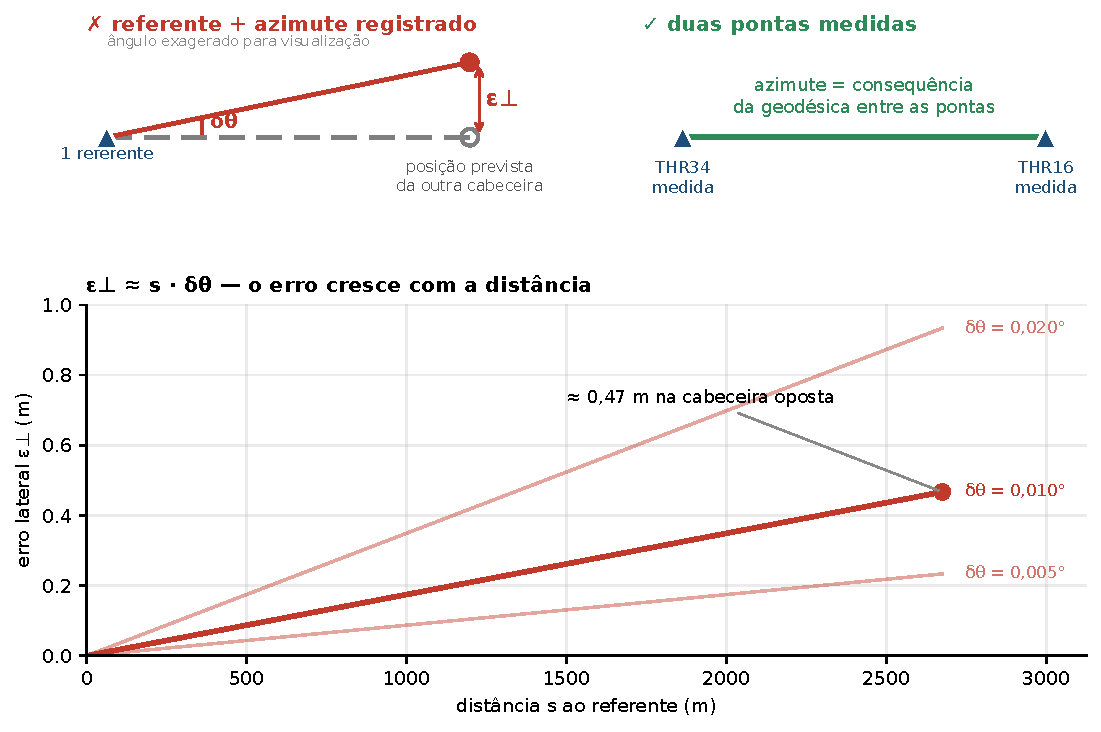
\includegraphics[width=\linewidth]{Figures/fig-erro-angular.pdf}
    \caption{Posicionamento por um referente e um azimute registrado, comparado ao posicionamento por duas pontas medidas, e o erro lateral $\varepsilon_\perp \approx s\,\delta\theta$ ao longo da pista do SBSJ. O ângulo do esquema superior está exagerado.}
    \label{fig:erro-angular}
    \par\smallskip{\small Fonte: o autor.}
\end{figure}

Referentes adicionais, como marcos geodésicos ou pontos de mudança de greide do perfil longitudinal, reduzem a distância entre uma posição e o ponto medido mais próximo (Figura~\ref{fig:referentes-adicionais}), mas também oferecem redundância. A distância calculada entre dois referentes pode ser comparada com a medida em campo, e uma divergência indica que uma das medições precisa ser verificada.

\begin{figure}[htbp]
    \centering
    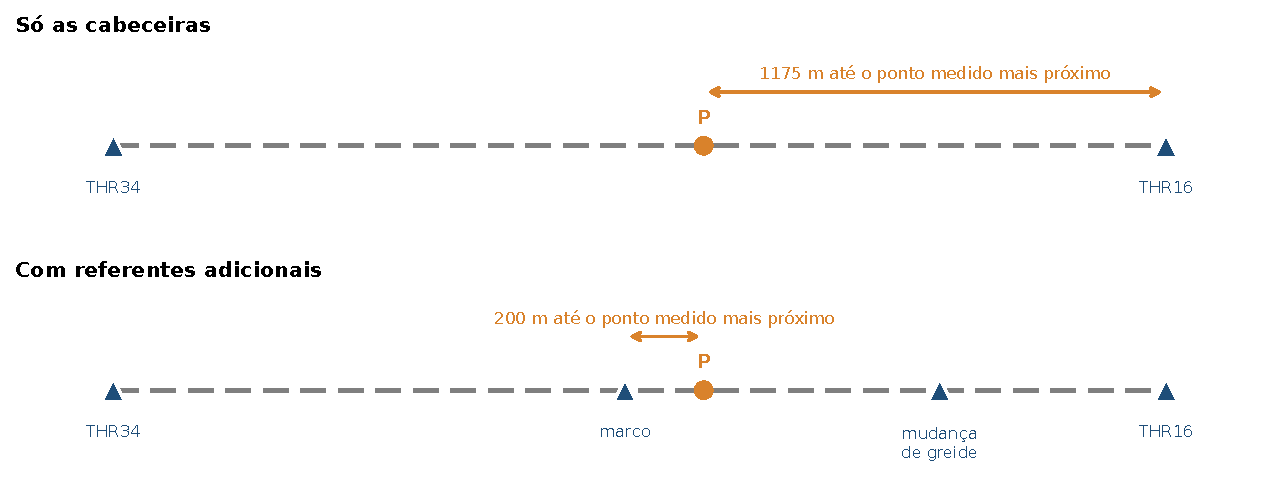
\includegraphics[width=\linewidth]{Figures/fig-referentes-adicionais.pdf}
    \caption{Efeito de referentes adicionais sobre a distância entre uma posição e o ponto medido mais próximo. As posições do marco e da mudança de greide são ilustrativas.}
    \label{fig:referentes-adicionais}
    \par\smallskip{\small Fonte: o autor.}
\end{figure}

\subsection{Plano e altitude}\label{sec:plano-altitude}

A arquitetura trata o plano e a altitude separadamente, como a geodésia faz com a planimetria e a altimetria. No plano, $s$ e $o$ são distâncias geodésicas sobre o elipsoide GRS80, adotado pelo SIRGAS2000, e não distâncias sobre uma projeção cartográfica (Seção~\ref{sec:geodesia}). Na carta de aeródromo do SBSJ, por exemplo, a diferença entre o norte da quadrícula e o norte verdadeiro é de cerca de $0{,}33^\circ$. A geodésica sobre o elipsoide dispensa essas convenções e serve, por isso, de régua comum a qualquer produto. Na altitude, a referência é a do próprio referente, e $v$ é uma diferença de altitude a partir dele.

Essa separação tem uma consequência que precisa ser declarada. Um comprimento calculado sobre o elipsoide não é o comprimento medido sobre o pavimento, e as reduções de altitude e de inclinação os separam (Equações~\ref{eq:reducao-altitude} e~\ref{eq:reducao-inclinacao}). Na pista do SBSJ, a uma altitude de cerca de 630~m e com desnível de 27,7~m, as duas reduções somam cerca de 0,4~m em 2675~m, sendo aproximadamente 0,26~m devidos à altitude e 0,14~m à inclinação (Figura~\ref{fig:plano-altitude}). A arquitetura fixa como convenção o comprimento sobre o elipsoide e a declara como parte da regra de derivação, para que dois produtos nunca misturem convenções. Quando um produto precisar das correções, elas são outros valores derivados, calculados a partir das altitudes dos referentes.

\begin{figure}[htbp]
    \centering
    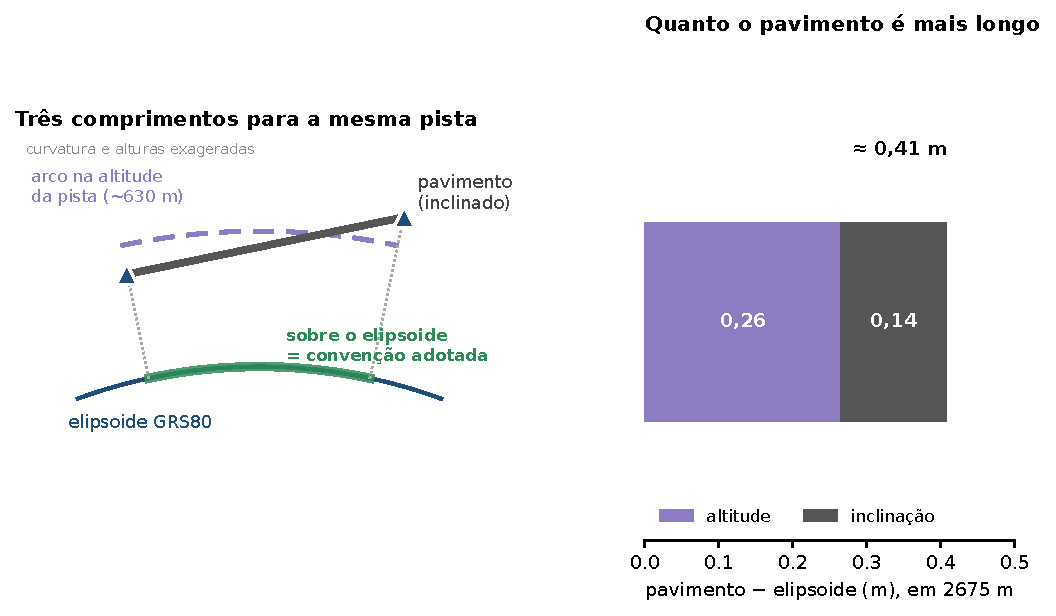
\includegraphics[width=\linewidth]{Figures/fig-plano-altitude.pdf}
    \caption{Comprimento sobre o elipsoide, na altitude da pista e sobre o pavimento inclinado, e as reduções de altitude e de inclinação na pista do SBSJ. Curvatura e alturas do esquema estão exageradas.}
    \label{fig:plano-altitude}
    \par\smallskip{\small Fonte: o autor.}
\end{figure}

\subsection{Remedição como evento}

Como nenhuma \textit{seed} guarda coordenadas nem comprimentos, a remedição de uma cabeceira é registrada em três passos (Figura~\ref{fig:remedicao-evento}). O primeiro é um evento que registra o levantamento, como \textit{feature} própria. O segundo é a publicação de um referencial com a nova posição da cabeceira. O terceiro é um \texttt{DELTA} na \textit{feature} \texttt{airport} que troca o \texttt{ref\_id}, com causa no levantamento. A pista, a zona de parada e as distâncias declaradas acompanham a mudança na leitura seguinte, e o histórico mostra por que mudaram.

\begin{figure}[htbp]
    \centering
    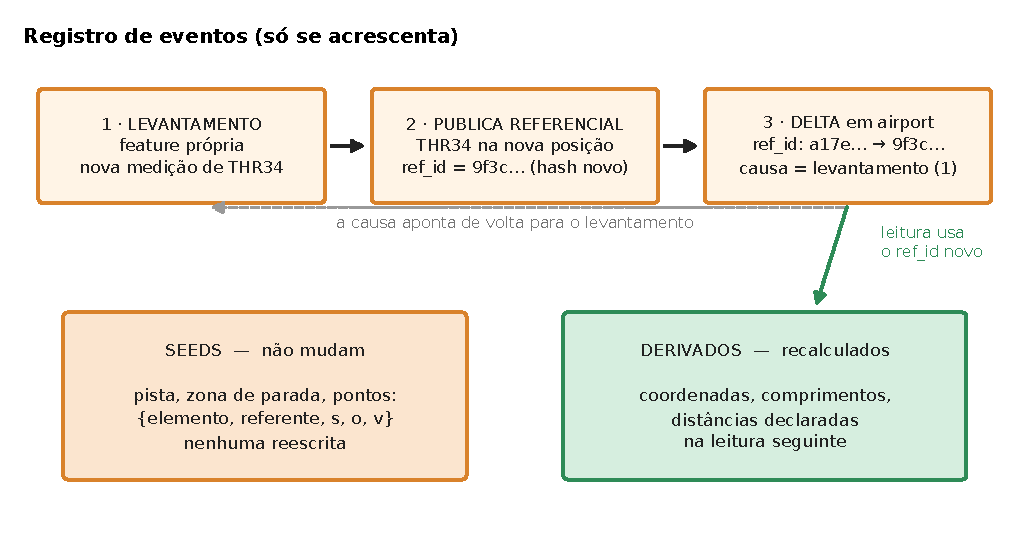
\includegraphics[width=\linewidth]{Figures/fig-remedicao-evento.pdf}
    \caption{Remedição de uma cabeceira como sequência de eventos: as \textit{seeds} permanecem inalteradas e os valores derivados são recalculados a partir do novo referencial. Os identificadores são ilustrativos.}
    \label{fig:remedicao-evento}
    \par\smallskip{\small Fonte: o autor.}
\end{figure}

\subsection{Geometria}

A geometria das \textit{features} também é derivada. Ela é gerada a partir das \textit{seeds}, com primitivos simples (ponto, retângulo e coroa), em um plano local em metros centrado em um dos referentes (Figura~\ref{fig:geometria-derivada}). A geometria serve para desenhar a carta a partir do registro, mas não integra as propriedades avaliadas.

\begin{figure}[htbp]
    \centering
    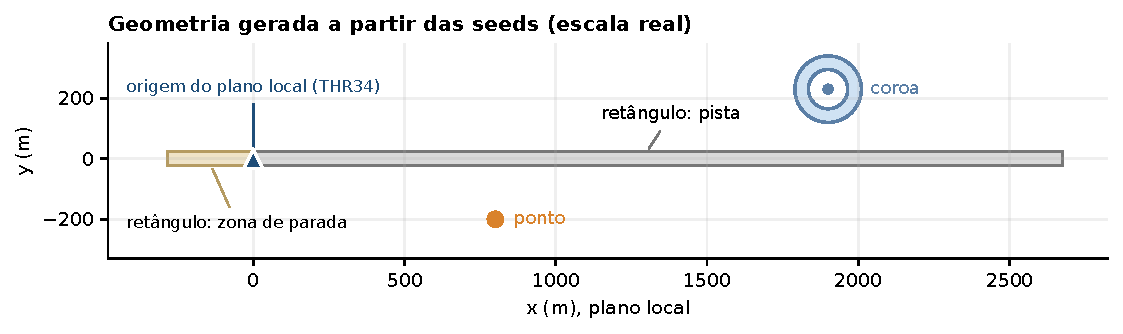
\includegraphics[width=\linewidth]{Figures/fig-geometria-derivada.pdf}
    \caption{Geometria gerada a partir das \textit{seeds} no plano local com origem em THR34. O ponto e a coroa são ilustrativos.}
    \label{fig:geometria-derivada}
    \par\smallskip{\small Fonte: o autor.}
\end{figure}

\section{A escrita}\label{sec:escrita}

\subsection{Forma e domínio}

A escrita tem apenas duas operações, a gravação de um evento e a gravação de um grupo. Ambas recusam, sem gravar nada, tudo o que viola a forma do registro, isto é:
\begin{itemize}
    \item tipo de evento inválido;
    \item \texttt{DELTA} ou \texttt{VOID} sem \texttt{BASELINE} vigente;
    \item \texttt{BASELINE} sobre \textit{feature} viva;
    \item envelope alterado;
    \item \texttt{VOID} sem motivo;
    \item autor vazio;
    \item caminho malformado, remoção de campo ausente e campo que seja ao mesmo tempo valor e prefixo de outro;
    \item causa que aponte para evento inexistente;
    \item posição que aponte para referente inexistente;
    \item troca de referencial que deixe alguma posição sem apoio.
\end{itemize}
Se qualquer evento de um grupo for recusado, nenhum é gravado, visto que são envoltos por uma transação de banco de dados.

A escrita não julga o domínio, como a plausibilidade de uma largura ou o atendimento de uma distância declarada à norma, a separação é deliberada. Um registro que interpretasse o domínio ficaria preso às regras vigentes no momento da gravação e não permitiria reavaliar o histórico com regras novas. Os juízos de domínio ficam do lado da leitura, onde podem mudar sem afetar o passado.

\subsection{Encadeamento por \textit{hash}}

Cada evento guarda o \textit{hash} do evento anterior na mesma cadeia e o seu próprio \textit{hash} (Seção~\ref{sec:adulteracao}), calculado como
\begin{equation}
    h_i = \mathrm{SHA\text{-}256}\big(\mathrm{JCS}(\mathit{env}_i,\, h_{i-1},\, C_i)\big)
    \label{eq:hash}
\end{equation}
em que $\mathit{env}_i$ é o envelope completo do evento, incluindo o identificador, o autor, o motivo, a causa e, quando houver, os campos do grupo. O termo $h_{i-1}$ é o \textit{hash} do evento anterior, e $C_i$ é a lista de campos do corpo, ordenada pelo caminho. JCS é a forma canônica de JSON definida na RFC~8785 \cite{rfc8785}, que fixa a ordem das chaves, a ausência de espaços e a representação dos números. Os campos do grupo só entram quando presentes, de modo que um evento fora de grupo não carrega campos vazios no \textit{hash}.

A forma canônica é o que permite a um terceiro refazer o cálculo em outra linguagem e chegar ao mesmo resultado. Sem ela, o mesmo conteúdo admitiria várias serializações, com \textit{hashes} diferentes. Como a causa, o autor e o grupo entram no \textit{hash}, trocar a causa de um evento ou retirá-lo de um grupo quebra a cadeia da mesma forma que trocar qualquer valor.

O referencial fica fora da cadeia, guardado à parte, mas está protegido de forma indireta. O seu identificador é o \textit{hash} do seu conteúdo, e esse identificador está no evento da \textit{feature} \texttt{airport}, que pertence à cadeia. Alterar o conteúdo de um referencial faz com que o identificador deixe de conferir, e trocar o identificador exige alterar um evento da cadeia.

\subsection{Serialização}

A escrita é serializada por cadeia, com um único ponto de ordenação por aeródromo. Com isso, a ordem dos eventos, a dos identificadores e a da cadeia coincidem sem nenhum cuidado adicional, e um grupo é contíguo por construção. Para o volume de um aeródromo, com poucas escritas por ciclo AIRAC, essa solução é suficiente, assim, a escrita privilegia a consistência. O ponto de ordenação pode ficar indisponível por algum tempo, mas nunca grava fora de ordem. As formas de receber escritas de várias fontes simultaneamente estão entre as propostas da Seção~\ref{sec:extensoes}.

\section{A leitura no registro}\label{sec:leitura}

\subsection{Estado em um instante}

O estado de uma \textit{feature} em $t$ é a composição dos seus eventos até $t$, a partir do \texttt{BASELINE} do ciclo de vida vigente. Como o corpo está em linhas, essa composição se reduz a uma única consulta. Para cada caminho, toma-se o valor do evento mais recente até $t$, sobre um índice ordenado por \textit{feature}, caminho e evento, e os campos removidos saem do resultado. A leitura pode restringir-se a uma camada por meio de um intervalo de caminhos no mesmo índice. A lista das \textit{features} vivas em $t$ é obtida com custo proporcional ao número de \textit{features}, e não ao de eventos.

Além do estado, o registro responde à diferença entre dois instantes, com os campos que mudaram e os valores anteriores e posteriores. Responde também ao envelope de qualquer evento, com o autor, o instante, o motivo e a causa, e aos ciclos de vida de uma \textit{feature}. São essas as perguntas de um auditor.
\begin{figure}[htbp]
    \centering
    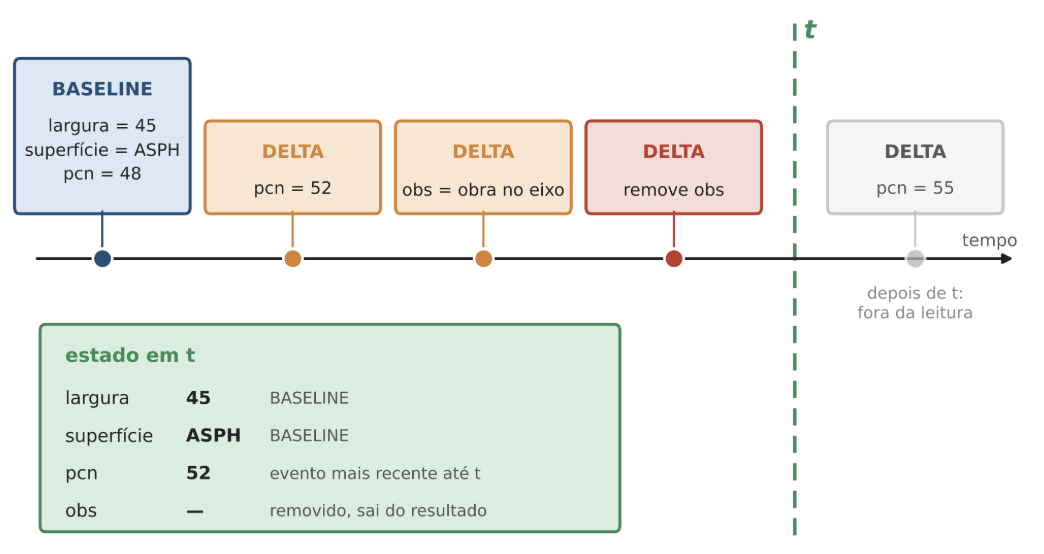
\includegraphics[width=1\linewidth]{Figures/estado-instante.png}
    \caption{Estado de uma \textit{feature} em $t$: composição do \texttt{BASELINE} com os eventos até $t$, tomando para cada caminho o valor mais recente e excluindo os campos removidos. Os valores são ilustrativos.}
    \label{fig:estado-instante}
    \par\smallskip{\small Fonte: o autor.}
\end{figure}
\subsection{Valores derivados}\label{sec:derivados}

O requisito do mínimo de informação (Seção~\ref{sec:req-minimo}) é atendido calculando na leitura tudo o que pode ser calculado. Valores como comprimento, azimute, rumo magnético e distâncias declaradas não são gravados. O comprimento e os azimutes resultam da geodésica entre os referentes, e o rumo magnético, do azimute e da variação magnética registrada no aeródromo. As distâncias declaradas resultam das definições do Anexo~14 (Seção~\ref{sec:distancias}), aplicadas ao estado no instante pedido:
\begin{equation}
    \begin{aligned}
        \mathrm{TORA} &= L, & \mathrm{TODA} &= L + \mathrm{CWY},\\
        \mathrm{ASDA} &= L + \mathrm{SWY}, & \mathrm{LDA} &= L - d,
    \end{aligned}
    \label{eq:distancias-declaradas}
\end{equation}
em que $L$ é o comprimento da pista, CWY e SWY são os comprimentos da zona livre de obstáculos e da zona de parada aplicáveis àquela direção, também calculados a partir das \textit{seeds}, e $d$ é o deslocamento da cabeceira, registrado como premissa da direção.

O cálculo é recusado, em vez de estimado, quando falta uma premissa estrutural. Sem referencial vigente, não há derivado, e uma \textit{seed} incompleta já é recusada na escrita. Pela mesma razão, um caso para o qual não há regra definida, como uma pista com barreira de contenção, leva à recusa, e não a um número possivelmente errado. Sem a norma de preenchimento proposta na Seção~\ref{sec:extensoes}, porém, o registro não distingue ``não se aplica'' de ``não informado''. A ausência de uma zona de parada, de uma zona livre de obstáculos ou de um deslocamento é lida como zero.

\subsection{Modelos de leitura e caches}

Cópias podem acelerar a leitura sem se tornar fonte de verdade. Uma delas é o estado de uma \textit{feature} ao fim de um evento, a partir do qual se aplicam apenas os eventos posteriores. Outra é o resultado de uma seleção por tipos e camadas em $t$, identificado por uma marca d'água, que é o maior \texttt{event\_id} até $t$ entre os eventos dos tipos selecionados. Um evento fora da seleção não move a marca e não invalida a cópia. Essas cópias podem ser apagadas a qualquer momento, e nenhuma escrita as lê. Um valor derivado pode, assim, ser guardado para acelerar a leitura, desde que essa cópia nunca sirva de premissa para outro cálculo.

A lente da carta de aeródromo é um exemplo de modelo de leitura. Ela monta o conteúdo de uma ADC em $t$ lendo apenas as camadas \texttt{adc} e \texttt{geometria} dos tipos que a carta mostra. Tudo o mais que o registro guarda, como os levantamentos, fica de fora sem ser lido. A tabela de distâncias da lente resulta da mesma regra da Equação~\ref{eq:distancias-declaradas}, sobre o mesmo referencial vigente. É dessa forma que se atende ao requisito de consistência entre produtos (Seção~\ref{sec:req-consistencia}). A carta e a tabela não guardam valores próprios, e duas leituras para o mesmo instante partem das mesmas afirmações.

\section{A distribuição da leitura}\label{sec:distribuicao}

Se todo produto for lido diretamente do banco, o banco passa a ser um ponto único de falha da leitura, e cada consulta concorre com a escrita. A distribuição separa as duas funções. O registro é publicado, na ordem em que foi gravado, em um único tópico, e cada consumidor monta, do seu lado, os modelos de leitura de que precisa. A Figura~\ref{fig:distribuicao} mostra o fluxo.

\begin{figure}[htbp]
    \centering
    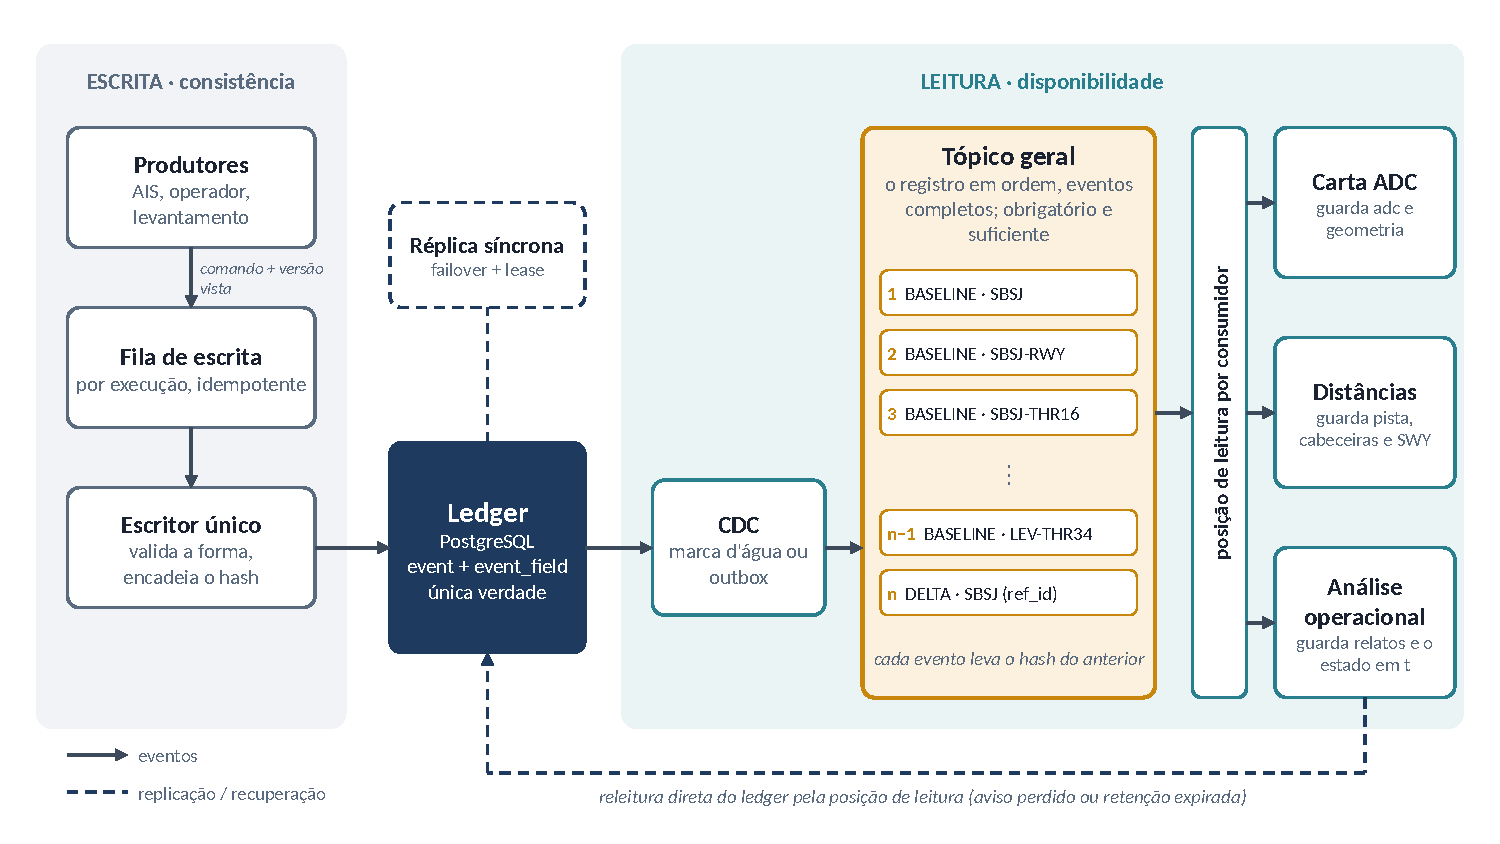
\includegraphics[width=\linewidth]{Figures/fig_arquitetura_pubsub.pdf}
    \caption{Distribuição da leitura. O registro é publicado em ordem em um tópico geral, e cada consumidor monta a sua projeção. Tudo à direita do registro é derivado e pode ser reconstruído a partir dele. A fila de escrita e a réplica síncrona, à esquerda, são extensões propostas (Seção~\ref{sec:extensoes}).}
    \label{fig:distribuicao}
    \par\smallskip{\small Fonte: o autor.}
\end{figure}

\subsection{O tópico geral}

O tópico geral é o próprio registro de um aeródromo, publicado evento a evento, com envelope e corpo, fora do banco. Ele é alimentado por um retransmissor que lê os eventos em ordem de \texttt{event\_id} e os anexa ao tópico, como em uma captura de mudanças (Seção~\ref{sec:distribuidos}). O retransmissor não guarda estado próprio, e o ponto de onde continua é o último evento já presente no tópico. Executá-lo novamente não duplica nada, e um tópico perdido é refeito do zero a partir do registro. O retransmissor também não espera nenhum consumidor. Antes do evento que adota um referencial, ele publica o corpo desse referencial, endereçado pelo conteúdo, de modo que o tópico é suficiente para quem o lê.

Há um único tópico, com todos os eventos, e todo consumidor o lê. Essa escolha mantém a camada mínima por quatro razões:
\begin{itemize}
    \item o consumidor recebe todos os eventos e, portanto, confere cada \textit{hash} e cada ligação, de ponta a ponta;
    \item os eventos de um grupo chegam juntos e em ordem, na mesma sequência, sem partes de uma mudança espalhadas por tópicos diferentes;
    \item o estado do consumidor reduz-se a uma única posição de leitura, o último evento aplicado;
    \item não há nada a rotear, e o encerramento de uma \textit{feature} é apenas mais um evento no tópico, como no registro.
\end{itemize}


\subsection{Canal não confiável}

O tópico pode estar hospedado em um intermediário que não está sob o
controle do leitor. Embora um sistema de mensageria possa tratar falhas de
entrega, como perda ou duplicação de mensagens, ele não garante que o evento
publicado esteja correto nem que seu conteúdo permaneça inalterado no
intermediário. Por isso, antes de aplicar um evento, o consumidor recalcula
seu \textit{hash}, conforme a Equação~\ref{eq:hash}, e verifica se o
\textit{hash} anterior declarado corresponde ao do último evento aplicado.
Além disso, confere se cada referencial recebido corresponde ao endereço
esperado.

Ao encontrar a primeira mensagem que falha em alguma dessas verificações,
o consumidor interrompe o processamento e não aplica nenhum evento
subsequente. Se o encadeamento de \textit{hashes} não corresponder ao
esperado, não é possível determinar, apenas com essa verificação, se o evento
recebido foi adulterado ou se a inconsistência está no último evento
aplicado. O consumidor deve, então, recuperar o último ponto de concordância
entre os eventos, caso o evento recebido permita estabelecer essa ligação,
ou descartar o último evento aplicado. Em ambos os casos, a recuperação
preserva apenas um prefixo do histórico cuja integridade não depende da
mensagem suspeita. Mensagens idênticas a eventos já aplicados são
reconhecidas como duplicatas e ignoradas.

\subsection{Consumidores}

Os consumidores são preguiçosos (\textit{lazy}) por definição. Não recebem requisições, não precisam estar sempre ativos e não precisam acompanhar o registro em tempo real. Um consumidor lê o tópico a partir da sua posição de leitura, no seu próprio ritmo, seja em laço, por agendamento ou uma única vez. Em seguida, confere e aplica o que leu e grava a nova posição. Ao ser retomado após uma queda, confere novamente o que já tinha. A Figura~\ref{fig:consumidor} mostra esse ciclo.

\begin{figure}[htbp]
    \centering
    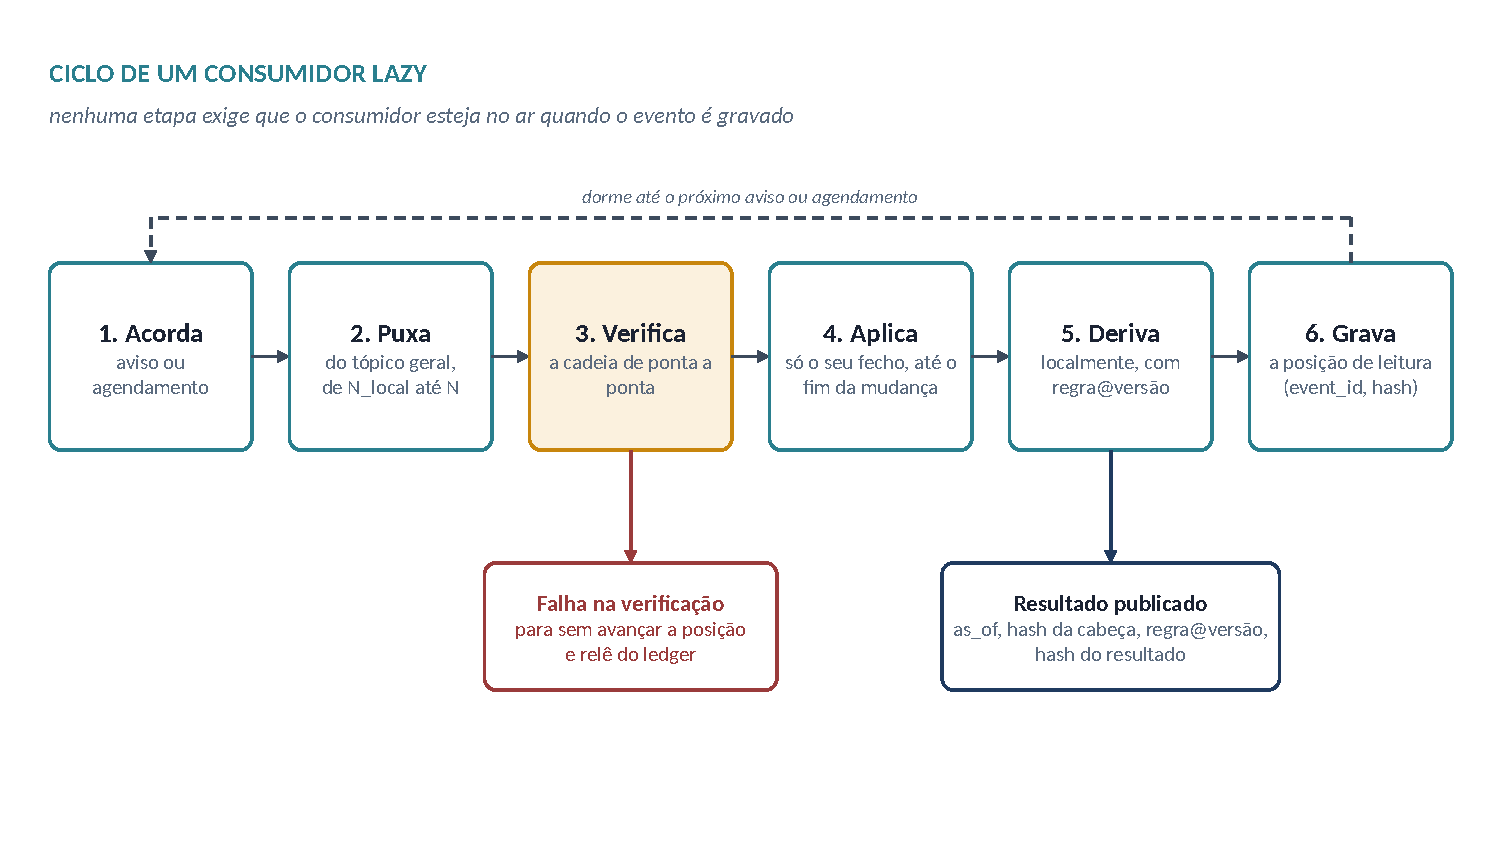
\includegraphics[width=\linewidth]{Figures/fig_ciclo_consumidor.pdf}
    \caption{Ciclo de um consumidor preguiçoso.}
    \label{fig:consumidor}
    \par\smallskip{\small Fonte: o autor.}
\end{figure}

Três regras preservam os requisitos da Seção~\ref{sec:requisitos} nesse cenário. A primeira é a do grupo inteiro, com os eventos de um grupo só são aplicados juntos, e, se o lote lido termina no meio de um grupo, o consumidor continua lendo até fechá-lo. Se o restante ainda não chegou, a posição não se move, ou seja, um corte de leitura nunca cai dentro de um grupo, e nenhuma leitura mostra uma carga pela metade.

A segunda regra é a do limite explícito. Toda leitura declara até onde vai, como \texttt{event\_id} ou como instante, e não existe leitura ``do mais recente''. Se o limite ultrapassa o que o consumidor já recebeu, ele recusa a leitura em vez de responder com um estado desatualizado.

A terceira regra é a da regra identificada. Como cada consumidor calcula os seus próprios derivados, a consistência entre produtos passa a depender de que todos apliquem a mesma regra. A regra é identificada pelo \textit{hash} do código que deriva os valores, e a resposta a declara.

\subsection{O recorte de cada consumidor}

Cada consumidor armazena todos os eventos recebidos, dado o baixo volume de
escritas, mas, ao construir uma resposta, considera apenas o fecho de
dependências das \textit{features} assinadas. Esse fecho percorre, nos dois
sentidos, as relações declaradas entre elementos, incluindo
\texttt{owner\_ref} e os campos que identificam outras \textit{features}.
Para elementos posicionados, considera também a ligação ao aeródromo, cujo
referencial determina o posicionamento. O campo \texttt{caused\_by} não
participa do fecho, pois relaciona eventos, não elementos. Relações
espaciais, como vizinhança e sobreposição, também não são armazenadas:
quando necessárias, são calculadas sobre o recorte selecionado.

Assim, a inscrição na cabeceira~16 alcança a pista, a cabeceira oposta, a
zona de parada, as restrições associadas e o aeródromo. O levantamento fica
de fora, pois sua única ligação com os demais elementos é por
\texttt{caused\_by}. Embora o aeródromo integre o fecho, suas demais relações
não são percorridas, evitando incluir todos os elementos nele posicionados.
Como todos os eventos são recebidos, novas \textit{features} que satisfaçam
essas relações, como uma barreira de contenção vinculada à pista, entram no
recorte sem exigir um mecanismo adicional de descoberta.

A resposta é um dado serializável que reúne o limite efetivo da leitura, a
cabeça da cadeia nesse limite, as \textit{features} assinadas, o fecho, os
estados, o referencial, os derivados, a regra aplicada e o \textit{hash} do
conjunto. Recusas também são representadas como respostas, na ausência de
referencial vigente, os derivados são substituídos pela indicação ``sem
referencial vigente''. Consumidores que aplicam a mesma regra ao mesmo
limite produzem o mesmo \textit{hash}; diferenças entre regras tornam as
divergências explícitas e atribuíveis, em vez de silenciosas.

\subsection{Disponibilidade e consistência}

Diante do compromisso descrito pelo teorema CAP (Seção~\ref{sec:distribuidos}), a arquitetura faz uma escolha em cada ponta. A escrita privilegia a consistência (Seção~\ref{sec:escrita}). A leitura privilegia a disponibilidade, com consumidores independentes que continuam respondendo com o banco fora do ar e que podem estar atrasados.

O atraso não leva a respostas diferentes. Como o registro só cresce, todo consumidor guarda um prefixo íntegro dele. Uma leitura com limite explícito tem, então, apenas duas respostas possíveis em qualquer consumidor. Ou seja, se ele já aplicou o registro até aquele limite, a resposta é a mesma de todos os outros; caso contrário, não há resposta. Um consumidor atrasado pode desconhecer um evento recente, mas não pode responder de forma diferente sobre um limite que já conhece.

\section{Verificação por terceiro}\label{sec:verificacao}

\subsection{Uma especificação pública}

O requisito de verificação por terceiros (Seção~\ref{sec:req-verificacao}) exige que quem recebe os dados possa conferi-los sem confiar em quem os entrega. Para isso, a especificação da cadeia (Equação~\ref{eq:hash}) é pública e curta. Qualquer pessoa pode escrever o seu próprio verificador, sem o código de quem publicou e esse verificador recalcula cada \textit{hash}, confere cada ligação e confere o identificador de cada referencial.

A mesma verificação aparece em três pontos da arquitetura. O registro verifica a si mesmo, o consumidor verifica cada mensagem do tópico, e qualquer verificador externo verifica o registro exportado e o banco extraído (Seção~\ref{sec:banco-extraido}). 

\subsection{Âncora externa}

O encadeamento denuncia qualquer alteração que deixe um sucessor. Alterar, apagar ou inserir um evento no meio do registro, ou uma mensagem no meio do tópico, quebra a cadeia a partir daquele ponto, mesmo que o atacante recalcule o \textit{hash} do evento alterado. Há, porém, alterações que não deixam sucessor para denunciá-las. No banco, é o caso de modificar apenas o último evento, truncar o final ou reescrever a cadeia inteira, recalculando todos os \textit{hashes}. No tópico, é o caso de cortar o fim, o que se confunde com atraso, ou anexar ao fim um evento falso que se liga corretamente ao último verdadeiro.

Essas alterações só são detectadas comparando a cabeça da cadeia, formada pelo último \texttt{event\_id} e pelo seu \textit{hash}, com uma âncora guardada fora do banco (Seção~\ref{sec:adulteracao}). O registro e o consumidor expõem a cabeça para esse fim, e o armazenamento e a comparação da âncora estão entre as propostas (Seção~\ref{sec:extensoes}). O encadeamento prova, portanto, que nada do que se recebeu foi alterado, mas não que se recebeu tudo.

\subsection{Cadeia linear e árvore de Merkle}

A árvore de Merkle oferece provas curtas de inclusão e de consistência (Seção~\ref{sec:adulteracao}), enquanto, na cadeia linear, o verificador refaz o percurso inteiro. Para o volume de um aeródromo, refazer o percurso tem custo baixo, e a cadeia é mais simples de especificar e de reimplementar, o que favorece justamente a verificação por terceiros. A árvore passa a valer a pena quando o registro cresce muito, ou quando é preciso provar um evento isolado a quem não deve receber o restante.

\section{O banco extraído}\label{sec:banco-extraido}

O registro é mantido em um banco servido, responsável pelas operações de
escrita e distribuição. Seu uso, entretanto, não deve depender do acesso a
esse servidor. Por isso, o produto final da arquitetura é um banco extraído:
um único arquivo SQLite~\cite{sqlite} que contém o registro completo de um
aeródromo. O banco do SBSJ é disponibilizado como conjunto de dados aberto
\cite{aeroledger_dataset}, acompanhado de cópias em CSV das principais
tabelas e visões para facilitar a inspeção.

Enquanto a AIP apresenta os valores vigentes, o banco
preserva as afirmações que lhes dão origem, incluindo autor, motivo, causa
e \textit{hash}. Dessa forma, os dados e as evidências de sua integridade
podem ser verificados por terceiros sem acesso ao banco servido, desde que
obtenham, por um canal independente, o \textit{hash} da cabeça da cadeia.

\subsection{Esquema}

O esquema espelha o do registro, com o envelope em colunas e o corpo em JSONB, o formato binário de JSON do SQLite. O arquivo contém quatro tabelas:
\begin{itemize}
    \item \texttt{exportacao}, com a procedência do arquivo e o aviso de que parte do cenário é simulada;
    \item \texttt{run}, com as cadeias contidas no arquivo;
    \item \texttt{referencial}, com o corpo de cada referencial, endereçado pelo conteúdo;
    \item \texttt{evento}, com o envelope em colunas e o corpo como a lista de linhas, cada uma com caminho, operação e valor, ordenada pelo caminho, exatamente a que entra no \textit{hash}.
\end{itemize}

Gatilhos (\textit{triggers}) do banco impedem a atualização e a exclusão de eventos, exigem o encadeamento e conferem a forma das linhas do corpo, e visões (\textit{views}) de leitura completam o arquivo. A visão \texttt{evento\_legivel} apresenta o instante extraído do próprio identificador, e a visão \texttt{campo}, o corpo achatado, com uma linha por campo. A visão \texttt{cabeca} mostra o último evento de cada cadeia, para comparação com a âncora, e a visão \texttt{estado\_atual}, as \textit{features} vivas e os seus campos. O arquivo traz ainda consultas de exemplo comentadas, que mostram o estado em um corte, o que mudou entre dois cortes, a trilha de causa de um evento e o referencial vigente. O esquema completo está no Apêndice~\ref{ape:ddl}.

Para isso, a exportação deve ser fiel, com os mesmos eventos, \textit{hashes} e cabeça do registro, e o mesmo estado em qualquer corte. Ficam fora do arquivo os derivados, que nunca são gravados, e as garantias da escrita, como a recusa de eventos malformados, que pertencem ao ponto de entrada, e não a um arquivo pronto.



\section{Implementação}\label{sec:implementacao}

A arquitetura foi implementada na biblioteca \texttt{aeroledger}, versão 0.6.0 (\textit{commit} \texttt{e93b718}) \cite{aeroledger}. A biblioteca é escrita em Python~3.12 sobre PostgreSQL~14 ou superior, com \texttt{psycopg} para o acesso ao banco, \texttt{pyproj} para a geodésia e \texttt{shapely} para a geometria. A biblioteca é o objeto avaliado. Os experimentos a utilizam como qualquer usuário a utilizaria, e cada passo corresponde a uma chamada a ela. A Tabela~\ref{tab:implementacao} relaciona as peças da arquitetura aos componentes da biblioteca.

\begin{table}[htbp]
    \centering
    \caption{Peças da arquitetura e a sua implementação no \texttt{aeroledger}.}
    \label{tab:implementacao}
    \begin{tabularx}{\linewidth}{l X}
        \toprule
        Na arquitetura & No \texttt{aeroledger} \\
        \midrule
        Escrita (Seção~\ref{sec:escrita}) & funções \texttt{escrever} e \texttt{escrever\_grupo}, que validam a forma e gravam na mesma transação \\
        Registro (Seção~\ref{sec:registro}) & tabelas \texttt{event} (envelope) e \texttt{event\_field} (uma linha por campo do corpo), apenas com inserção; tabela \texttt{referencial}, endereçada pelo conteúdo \\
        Estado em $t$ (Seção~\ref{sec:leitura}) & \texttt{DISTINCT ON} sobre o índice (\textit{feature}, caminho, evento); varredura saltada do índice para listar as \textit{features} vivas \\
        Cópias de leitura & tabelas \texttt{snapshot} e \texttt{projecao\_cache} (marca d'água) \\
        Derivados & módulo \texttt{derivacoes}; erro \texttt{RegraPendente} para a pista com barreira de contenção \\
        Lente da carta & módulo \texttt{adc} \\
        Tópico geral e consumidores (Seção~\ref{sec:distribuicao}) & módulo \texttt{topico}, com \texttt{retransmitir}, \texttt{Consumidor} e \texttt{TopicoMemoria}; erros \texttt{TopicoCorrompido} e \texttt{ConsumidorAtrasado} \\
        Verificação (Seção~\ref{sec:verificacao}) & funções \texttt{verificar\_cadeia} e \texttt{cabeca} \\
        \bottomrule
    \end{tabularx}
    \par\smallskip{\small Fonte: o autor.}
\end{table}

A implementação difere da arquitetura em quatro pontos, que limitam o alcance dos experimentos:
\begin{itemize}
    \item a escrita é serializada por um bloqueio pessimista da linha da execução (\texttt{SELECT ... FOR UPDATE}), e as formas de escrita com várias fontes da Seção~\ref{sec:extensoes} não estão implementadas;
    \item o tópico é mantido em memória (\texttt{TopicoMemoria}), com o mesmo contrato que um sistema de mensagens cumpriria, isto é, anexar e ler a partir de uma posição;
    \item a regra das distâncias declaradas com barreira de contenção não está implementada, e a biblioteca recusa o cálculo quando há uma barreira viva;
    \item o motor de geometria é uma demonstração, que desenha a carta a partir do registro, mas não foi validado contra as cartas oficiais.
\end{itemize}

A biblioteca tem 57 testes próprios, sobre um aeródromo fictício, cada um executado em um banco descartável. Eles cobrem, entre outros aspectos, as recusas de escrita, as regras do referencial, os grupos e a equivalência entre a leitura com \textit{snapshot} e a reconstrução completa. Em relação aos grupos, verificam a contiguidade, a presença no \textit{hash} e a gravação de todos ou de nenhum dos eventos. Esses testes não integram a avaliação. Eles garantem que a biblioteca faz o que declara antes de ser avaliada sobre o SBSJ.

\section{Aplicação ao SBSJ}\label{sec:aplicacao-sbsj}

\subsection{Cenário}

Os experimentos usam duas cadeias. A cadeia \texttt{aixm} guarda a pista na forma em que as publicações chegam ao usuário e serve apenas ao E1. A cadeia \texttt{sbsj} guarda a pista no modelo proposto, com os dez eventos da Tabela~\ref{tab:eventos-sbsj}, na ordem em que os experimentos os escrevem. Essa ordem compreende a carga do eAIP como um grupo de cinco eventos (E2), a remedição da cabeceira~34 trinta dias depois (E2), uma interdição de três dias (E3) e uma restrição nova escrita durante o E6. Nenhum evento contém comprimento, azimute ou distância declarada, e todos esses valores são calculados na leitura (Seção~\ref{sec:derivados}). As premissas da carga vêm da AIP. A remedição e as restrições são simuladas, para exercitar o ciclo de vida.

\begin{table}[htbp]
    \centering
    \caption{Eventos que registram a pista do SBSJ.}
    \label{tab:eventos-sbsj}
    \begin{tabularx}{\linewidth}{l l l X}
        \toprule
        \# & \textit{Feature} & Evento & Conteúdo \\
        \midrule
        1--5 & \makecell[l]{SBSJ, SBSJ-RWY,\\ SBSJ-THR16,\\ SBSJ-THR34,\\ SBSJ-SWY} & \makecell[l]{\texttt{BASELINE},\\ em grupo} & carga do eAIP: aeródromo com referencial vigente e variação magnética; pista como retângulo entre as cabeceiras, com 45~m de largura; cabeceiras sobre os seus referentes; zona de parada de 283~m além da cabeceira~34 \\
        6 & SBSJ-LEV-THR34 & \texttt{BASELINE} & levantamento que remede a cabeceira~34 (simulado) \\
        7 & SBSJ & \texttt{DELTA} & troca do referencial, com causa no evento~6 \\
        8--9 & SBSJ-RES-0001 & \makecell[l]{\texttt{BASELINE},\\ \texttt{VOID}} & interdição de 300~m a partir da cabeceira~34, com a pista como dona, e o seu encerramento (NOTAM simulado) \\
        10 & SBSJ-RES-0002 & \texttt{BASELINE} & nova restrição na pista (NOTAM simulado) \\
        \bottomrule
    \end{tabularx}
    \par\smallskip{\small Fonte: o autor, a partir de \citeonline{decea2026aip}.}
\end{table}

O referencial tem os dois referentes georreferenciados, com as coordenadas e elevações da seção AD~2.12, e o elemento linear entre eles. A pista entra como um retângulo de 45~m de largura entre as cabeceiras. A zona de parada entra como um retângulo de 283~m a partir da cabeceira~34, aplicado à direção~16. A variação magnética é de $22^\circ$W. O número 2675 não é escrito em nenhum evento.

\subsection{Procedimentos dos experimentos}\label{sec:procedimentos}

As perguntas e os critérios de aprovação de cada experimento estão na Seção~\ref{sec:experimentos}. Esta seção descreve como cada um é executado sobre o cenário.

\paragraph*{E1: causa.} A cadeia \texttt{aixm} não emula o AIXM completo, apenas as duas edições que o usuário recebe, com cada número publicado guardado como campo e sem causa. A pista é registrada com os valores da AOC de 2022 e, em seguida, alterada com os da ADC de 2026, ambos afirmados pelo DECEA. Contam-se os campos que mudam e verifica-se se algum deles traz causa.

\paragraph*{E2: derivação.} Entram no registro apenas as premissas, isto é, as coordenadas e elevações das cabeceiras, a largura da pista e as dimensões da zona de parada. O comprimento, os azimutes, os rumos magnéticos e as distâncias declaradas são calculados e comparados com os valores da AIP. Em seguida, a cabeceira~34 é remedida, deslocada em cerca de 1~m. Conferem-se então os eventos escritos e os novos valores contra o gabarito de Vincenty.

\paragraph*{E3: reconstrução no tempo.} Após a remedição, uma interdição de 300~m a partir da cabeceira~34 entra como restrição, com a pista como dona, e é encerrada três dias depois. O banco é então consultado como um auditor faria, em instantes anteriores, intermediários e posteriores a cada mudança. São consultados:
\begin{itemize}
    \item o referencial vigente e o comprimento derivado;
    \item a existência da interdição;
    \item o envelope da troca de referencial;
    \item as distâncias declaradas recalculadas para um instante passado;
    \item a diferença entre dois instantes.
\end{itemize}
O instante $t_a$, logo após a carga do eAIP, serve de referência ao longo deste e dos experimentos seguintes.

\paragraph*{E4: evidência de adulteração.} O atacante tem acesso direto ao banco. Antes dos ataques, a cabeça da cadeia é anotada fora do banco, como âncora. São executados quatro ataques:
\begin{itemize}
    \item alterar o corpo de um evento sem recalcular o \textit{hash};
    \item apagar um evento;
    \item inserir um evento com \textit{hash} próprio correto;
    \item alterar um evento e recalcular todos os \textit{hashes} até o fim.
\end{itemize}
Cada ataque é executado em uma cópia do banco e conferido de duas formas, pela verificação interna da cadeia e pela comparação com a âncora.

\paragraph*{E5: consistência e verificação.} Dois produtos são gerados do mesmo banco, antes e depois da remedição. O primeiro é a tabela da AIP, com o comprimento e as distâncias declaradas, e o segundo, o conteúdo da carta de aeródromo. Em seguida, o registro é exportado em JSON e entregue ao verificador independente, primeiro intacto e depois com a largura da pista alterada em um metro no arquivo.

\paragraph*{E6: leitura separada.} O registro é retransmitido para o tópico, e as seis propriedades do E6 são exercitadas da seguinte forma:
\begin{itemize}
    \item \textbf{equivalência}: um consumidor lê todo o tópico, e as suas respostas são comparadas com as do banco em cada fronteira de corte do histórico e em três instantes, a saber, logo após a carga, durante a interdição e um segundo antes do seu fim;
    \item \textbf{atomicidade}: o banco e o consumidor são consultados com um limite que cai dentro da carga do eAIP, logo após a pista e antes da zona de parada;
    \item \textbf{recorte}: um consumidor que assina apenas a cabeceira~16 é comparado com o que lê tudo;
    \item \textbf{limite explícito e disponibilidade}: uma restrição nova é escrita no banco, e o consumidor é consultado sobre ela antes e depois de recebê-la, e novamente com o banco fechado;
    \item \textbf{determinismo}: seis consumidores leem o tópico de formas diferentes, e comparam-se os \textit{hashes} das respostas no mesmo limite. As formas são tudo de uma vez; em laço, uma mensagem por vez; em lotes de duas mensagens, menores que a carga; por agendamento; com uma queda no meio e retomada a partir de uma posição gravada em arquivo; e a partir de um tópico refeito do zero;
    \item \textbf{canal adulterado}: o atacante está no canal, e o banco não é tocado.
\end{itemize}

No canal adulterado, o alvo é a mensagem da troca de referencial, e alterá-la equivale a fazer o tópico afirmar que o referencial antigo continua vigente. São seis ataques:
\begin{itemize}
    \item trocar o referencial sem recalcular o \textit{hash};
    \item trocar o referencial e recalcular o \textit{hash} da mensagem;
    \item remover a mensagem;
    \item inserir depois dela um evento falso com ligação e \textit{hash} corretos;
    \item remover as últimas mensagens;
    \item anexar ao fim um evento falso com ligação e \textit{hash} corretos.
\end{itemize}

\subsection{Geração do banco extraído}

O banco extraído é gerado por um programa que escreve, por meio da biblioteca, o mesmo cenário dos experimentos em um PostgreSQL vazio. Em seguida, o programa exporta o resultado para SQLite com consultas SQL diretas, sem passar pela biblioteca, e confere o arquivo com o verificador independente.

A fidelidade da exportação é verificada de três formas. A primeira é a integridade e a cabeça das duas cadeias no arquivo. A segunda é o comprimento calculado pelo verificador a partir do referencial exportado. A terceira é a consulta de estado no SQLite, feita apenas com as visões do arquivo e comparada com a da biblioteca em todos os pares de corte e \textit{feature}.

\section{Extensões propostas}\label{sec:extensoes}

A arquitetura pode ser ampliada para atender a cenários de escrita
concorrente, padronização dos dados, distribuição em maior escala, consultas
mais expressivas e verificação independente do histórico. As extensões
descritas a seguir são propostas e não foram implementadas nem avaliadas
experimentalmente. Elas preservam o registro como fonte das afirmações,
acrescentando mecanismos nas etapas de escrita, distribuição ou leitura.

\subsection{Escrita com várias fontes}

A informação aeronáutica combina dados provenientes de diferentes agentes,
como operadores de aeródromos, órgãos de informação aeronáutica e equipes
de levantamento. Para acomodar essas fontes sem comprometer a ordem do
histórico, propõe-se um escritor único por cadeia, precedido por uma fila
de comandos. Cada comando recebe uma chave de idempotência, permitindo
reconhecer reenvios e evitar gravações duplicadas. O escritor valida os
comandos, registra os eventos em sequência e confirma sua aceitação ao
remetente.

A concorrência também pode ser controlada por \textit{feature}. Para
escrever, o agente informa o último \texttt{event\_id} que observou.
Se a \textit{feature} tiver sido alterada desde então, a operação é recusada
e o agente deve consultar o estado atualizado antes de tentar novamente.
Esse controle otimista evita que uma alteração seja aceita com base em
uma versão desatualizada. Uma restrição de unicidade sobre o par formado
pela cadeia e pelo \textit{hash} anterior reforça a prevenção de bifurcações
acidentais. A versão confirmada também pode identificar o limite de leitura
e compor a chave de cache, desde que esses mecanismos utilizem a mesma
definição de versão.

\subsection{Norma de preenchimento}

A flexibilidade do registro permite acomodar diferenças entre aeródromos,
mas não determina quais informações são necessárias para validar os dados
ou calcular os derivados. Propõe-se, por isso, uma norma de preenchimento
organizada em três camadas:
\begin{itemize}
    \item uma camada obrigatória, validada na escrita, que define os tipos
    dos elementos, as unidades, a origem dos valores e os requisitos
    mínimos para o cálculo dos derivados;
    \item uma camada recomendada, baseada no catálogo de dados aeronáuticos
    do PANS-AIM~\cite{icao2018pansaim}, que padroniza nomes e unidades;
    \item uma camada de extensão, identificada pelo prefixo \texttt{x\_},
    destinada a campos específicos. Campos recorrentes podem ser
    incorporados à camada recomendada em versões posteriores da norma.
\end{itemize}

A norma distingue três estados de ausência: ``não informado'',
``não se aplica'' e ``desconhecido''. Essa distinção impede que a falta
de uma premissa seja interpretada automaticamente como zero. Por exemplo,
se o deslocamento de uma cabeceira for necessário para um cálculo, sua
ausência deve resultar na recusa desse cálculo.

A norma é versionada para que cada evento possa ser interpretado segundo
as regras aplicáveis, sem reescrever o histórico. Assim, a estrutura do
registro preserva as afirmações originais, enquanto a interpretação
padronizada pode evoluir de forma reproduzível.

\subsection{Transporte e escala}

Para o volume de dados de um único aeródromo, o próprio banco pode atender
à distribuição dos eventos. Em cenários de maior escala, um sistema de
mensageria, como o Kafka~\cite{kreps2011kafka}, pode desacoplar a escrita
do consumo e distribuir os eventos entre diferentes leitores. A adoção
desse mecanismo, entretanto, não elimina a necessidade de verificar a
integridade e a continuidade da cadeia.

Duas estratégias podem reduzir o volume transmitido. Na primeira, o tópico
transporta apenas os envelopes dos eventos, e o consumidor busca no registro
os corpos necessários ao seu recorte, conferindo cada um contra o
\textit{hash} declarado. Essa abordagem reduz o tráfego, mas mantém a
dependência de acesso ao registro.

Na segunda, tópicos derivados distribuem eventos por \textit{feature} ou
por aeródromo, permitindo segmentar o fluxo conforme as necessidades de
cada consumidor. Como esses tópicos podem omitir eventos da cadeia original,
a verificação exige informações suficientes para detectar lacunas e
confirmar a ligação dos eventos recebidos ao histórico de origem.

\subsection{Consulta}

A distribuição define como os eventos chegam ao consumidor; a consulta
define como o estado reconstruído pode ser interrogado. Uma possibilidade
é utilizar GraphQL sobre a projeção local do consumidor. Nesse modelo,
a consulta especifica o limite de leitura, seleciona o fecho de dependências
e acessa as relações declaradas e os derivados calculados segundo a regra
aplicável.

Outra possibilidade é empregar uma linguagem de consulta lógica, como
Datalog, utilizada pelo Datomic~\cite{cognitect2026}. A escolha da linguagem
determina como as perguntas são expressas, mas não altera a origem dos
dados nem as regras de reconstrução do estado. Os resultados continuam
condicionados ao histórico verificado, ao recorte selecionado, ao limite
de leitura e à regra de cálculo utilizada.

\subsection{Dois eixos de tempo}

Uma extensão bitemporal, conforme discutido na
Seção~\ref{sec:bitemporal}, permitiria distinguir o tempo de transação,
controlado pelo sistema, do tempo de validade, declarado em cada afirmação.
Com isso, seria possível consultar tanto o estado conhecido pelo sistema
em determinado instante quanto o estado correspondente a um período de
validade específico.

Essa extensão também afeta a estratégia de consulta. Enquanto o tempo de
transação permite percorrer o histórico em ordem, as consultas por intervalos
de validade podem se beneficiar de índices especializados, como um índice
GiST sobre \texttt{tstzrange} no PostgreSQL. Quando o fim de um intervalo
puder ser inferido de afirmações posteriores, ele poderá ser calculado
durante a leitura, sem alterar afirmações anteriores.

\subsection{Âncora e prova de inclusão}

Para permitir a verificação independente do histórico, propõe-se publicar
o \textit{hash} da cabeça da cadeia a cada emenda AIRAC ou depositá-lo,
junto com o banco extraído, em um repositório com histórico verificável.
A comparação com uma referência obtida por um canal independente permitiria
detectar alterações posteriores ao estado ancorado, desde que a referência
publicada não pudesse ser substituída silenciosamente.

Quando for necessário comprovar a inclusão de um evento sem compartilhar
todo o registro, uma árvore de Merkle poderá fornecer uma prova compacta
de pertencimento a um conjunto comprometido. Essa estratégia seria útil,
por exemplo, no compartilhamento seletivo de dados operacionais entre
empresas. A prova demonstraria a inclusão do evento no conjunto
correspondente, mas não garantiria a veracidade de seu conteúdo.

\section{Limites conhecidos}\label{sec:limites-arq}

As limitações a seguir dizem respeito às garantias da arquitetura
apresentada. Restrições específicas do protótipo, como funcionalidades
não implementadas e limitações de desempenho, são discutidas na
Seção~\ref{sec:implementacao}.

\begin{itemize}
    \item \textbf{Autoria:} o campo \texttt{asserted\_by} identifica o autor
    por texto, mas não comprova sua identidade, pois a arquitetura não exige
    assinatura digital.

    \item \textbf{Integridade sem âncora externa:} a cadeia de
    \textit{hashes} permite verificar a consistência interna do histórico,
    mas não impede que alguém com controle sobre todo o registro o
    reescreva. Sem uma referência independente, também não é possível
    confirmar se o histórico recebido corresponde ao anteriormente
    publicado.

    \item \textbf{Interpretação dos dados:} sem uma norma de preenchimento,
    a ausência de um campo pode ser confundida com um valor válido, como
    zero. A distinção entre ausência, inaplicabilidade e desconhecimento
    depende da adoção de convenções explícitas.

    \item \textbf{Confidencialidade:} o tópico geral expõe os eventos nele
    publicados aos seus consumidores. O isolamento de dados restritos exige
    mecanismos adicionais, como fluxos separados e controles de acesso.
    A publicação de \textit{hashes}, isoladamente, não garante
    confidencialidade.

    \item \textbf{Escopo temporal e espacial:} cada cadeia representa um
    único aeródromo, e a ordenação de eventos entre aeródromos distintos
    não é definida. Além disso, o modelo atual utiliza apenas o tempo de
    transação; consultas pelo tempo de validade exigem uma extensão
    bitemporal.

    \item \textbf{Banco extraído:} o arquivo preserva o histórico registrado,
    mas não inclui necessariamente os derivados nem impede modificações
    diretas. Sua integridade depende de verificações realizadas sobre o
    conteúdo e de uma referência confiável para comparação.

    \item \textbf{Veracidade:} a integridade do histórico não garante que
    as medições estejam corretas. A arquitetura permite rastrear quem
    afirmou um valor, quando a afirmação foi registrada e de quais dados
    ela depende, mas a validação factual exige fontes e procedimentos
    externos.
\end{itemize}

\chapter{Resultados}\label{chap:resultados}
Este capítulo apresenta os resultados dos seis experimentos, na ordem em que foram definidos na Seção~\ref{sec:experimentos} e executados conforme a Seção~\ref{sec:procedimentos}. Para cada experimento, apresenta-se primeiro o que foi obtido e, em seguida, a resposta à pergunta correspondente. Todos os números provêm do \textit{notebook} executado \cite{aeroledger_experimentos}. A Seção~\ref{sec:res-banco} trata do banco extraído, a Seção~\ref{sec:res-sintese} reúne as respostas, e a Seção~\ref{sec:res-limites} discute os limites da avaliação.

\section{E1: causa}\label{sec:res-e1}

Entre a AOC de 2022 e a ADC de 2026, mudam doze campos (Tabela~\ref{tab:res-e1}), e nenhum deles traz causa. O registro informa quem publicou cada valor e em que edição, mas não por que o número mudou.

A alteração do comprimento da pista, de 2676 para 2675~m, aparece como sete números editados separadamente. Isso ocorre porque as distâncias declaradas estão guardadas, e não calculadas. As alterações da zona de parada e da faixa de pista não têm explicação em nenhuma das duas publicações.

\begin{table}[htbp]
    \centering
    \caption{E1: campos que mudam entre a AOC de 2022 e a ADC de 2026.}
    \label{tab:res-e1}
    \begin{tabular}{l r r}
        \toprule
        Campo & AOC 2213 (m) & ADC 2604 (m) \\
        \midrule
        Comprimento da pista & 2676 & 2675 \\
        Comprimento da zona de parada & 325 & 283 \\
        Comprimento da faixa & 3121 & 3118 \\
        Largura da faixa & 300 & 280 \\
        ASDA 16 & 3001 & 2958 \\
        TORA, TODA e LDA 16 & 2676 & 2675 \\
        TORA, TODA, ASDA e LDA 34 & 2676 & 2675 \\
        \bottomrule
    \end{tabular}
    \par\smallskip{\small Fonte: o autor, a partir de \citeonline{decea2022aoc} e \citeonline{decea2026adc}.}
\end{table}

A resposta à pergunta do E1 é, portanto, negativa. O modelo que guarda o valor publicado registra a mudança, mas não a sua causa.

\section{E2: derivação}\label{sec:res-e2}

Todos os valores calculados a partir das premissas ficam dentro da margem definida para cada grandeza (Tabela~\ref{tab:res-e2}), e nenhum campo de valor derivado está guardado no banco. A diferença de 0,342~m em todas as distâncias declaradas é a mesma do comprimento, como prevê a Equação~\ref{eq:distancias-declaradas}.

\begin{table}[htbp]
    \centering
    \caption{E2: valores calculados a partir das premissas e valores publicados.}
    \label{tab:res-e2}
    \begin{tabular}{l r r r r}
        \toprule
        Grandeza & Calculado & Publicado & Diferença & Margem \\
        \midrule
        Comprimento (m) & 2675,342 & 2675 & $+0{,}342$ & 0,919 \\
        Azimute 16 ($^\circ$) & 134,935 & 134,93 & $+0{,}005$ & 0,014 \\
        Azimute 34 ($^\circ$) & 314,927 & 314,92 & $+0{,}007$ & 0,014 \\
        Rumo magnético 16 ($^\circ$) & 156,935 & 157 & $-0{,}065$ & 1,009 \\
        Rumo magnético 34 ($^\circ$) & 336,927 & 337 & $-0{,}073$ & 1,009 \\
        TORA, TODA e LDA 16 (m) & 2675,342 & 2675 & $+0{,}342$ & 0,919 \\
        ASDA 16 (m) & 2958,342 & 2958 & $+0{,}342$ & 1,419 \\
        TORA, TODA, ASDA e LDA 34 (m) & 2675,342 & 2675 & $+0{,}342$ & 0,919 \\
        \bottomrule
    \end{tabular}
    \par\smallskip{\small Fonte: o autor, a partir de \citeonline{decea2026aip}.}
\end{table}

A remedição da cabeceira~34 gerou dois eventos. O primeiro registra o levantamento, com três campos. O segundo troca o referencial no aeródromo, com um único campo e o levantamento como causa. Nenhuma \textit{feature} com posição foi reescrita, seja a pista, as cabeceiras ou a zona de parada. O comprimento passou de 2675,342~m para 2676,195~m sem que nenhum número fosse digitado.

Os cantos da pista e da zona de parada coincidem com o gabarito de Vincenty a menos de 3,3~nm, tanto com o referencial antigo quanto com o novo. O novo comprimento coincide com o gabarito a menos de 0,1~\textmu m. Ambas as diferenças ficam muito abaixo da exatidão de 0,5~mm do próprio gabarito.

As duas perguntas do E2 têm, assim, resposta favorável à arquitetura. Os valores publicados se recalculam a partir das premissas dentro da precisão da AIP, e a troca de uma premissa não obriga a reescrever nenhum outro dado.

\section{E3: reconstrução no tempo}\label{sec:res-e3}

Em $t_a$, logo após a carga do eAIP, o referencial vigente é o original, e o comprimento derivado é de 2675,342~m. Ao fim do cenário, o referencial vigente é o novo, e o comprimento derivado passa a 2676,195~m.

A interdição aparece como existente no instante em que foi escrita, 36 horas depois e um segundo antes do encerramento. Não aparece um segundo antes de ser escrita, no instante do encerramento nem um dia depois. O seu ciclo de vida compõe-se exatamente de um \texttt{BASELINE} e de um \texttt{VOID}, sem nenhum tipo de evento específico para o caráter temporário.

O envelope da troca de referencial identifica o autor da afirmação (DECEA), o motivo (a remedição da cabeceira~34) e a causa (o levantamento, afirmado por outro autor). As distâncias declaradas calculadas depois da remedição para o instante $t_a$ são idênticas, \textit{bit} a \textit{bit}, às calculadas no próprio $t_a$. A diferença entre $t_a$ e o fim do cenário lista quatro campos, a saber, o identificador do referencial e os três campos do levantamento.

O E3 confirma, portanto, que qualquer instante é reconstruído a partir do histórico, com autor, motivo e causa de cada mudança.

\section{E4: evidência de adulteração}\label{sec:res-e4}

A Tabela~\ref{tab:res-e4} resume os quatro ataques ao banco. A alteração de um evento no meio da cadeia é apontada no próprio evento. A exclusão de um evento, ou a inserção de um evento novo com \textit{hash} próprio correto, é apontada no evento seguinte, que perde a ligação com o anterior. A reescrita da cadeia a partir do evento alterado, com o recálculo de todos os \textit{hashes}, passa pela verificação interna e só é detectada pela âncora.

\begin{table}[htbp]
    \centering
    \caption{E4: ataques ao banco e o que os detecta.}
    \label{tab:res-e4}
    \begin{tabularx}{\linewidth}{X l l}
        \toprule
        Ataque & Verificação interna & Âncora \\
        \midrule
        Alterar o corpo de um evento sem recalcular o \textit{hash} & aponta o evento & detecta \\
        Apagar um evento & aponta o seguinte & detecta \\
        Inserir um evento, com \textit{hash} próprio correto & aponta o seguinte & detecta \\
        Alterar um evento e recalcular todos os \textit{hashes} até o fim & não aponta & detecta \\
        \bottomrule
    \end{tabularx}
    \par\smallskip{\small Fonte: o autor.}
\end{table}

A resposta ao E4 é positiva, com um limite. Toda alteração no meio da cadeia é detectada pela verificação interna, mas a reescrita completa escapa a ela e só é detectada pela âncora externa.

\section{E5: consistência e verificação}\label{sec:res-e5}

Os dois produtos gerados do mesmo banco apresentam as mesmas distâncias em $t_a$, com ASDA~16 de 2958,342~m e LDA~34 de 2675,342~m. Ao fim do cenário, também coincidem, com 2959,195~m e 2676,195~m, e mudam juntos.

O verificador independente declara a cadeia íntegra. Ele chega à mesma cabeça que a biblioteca e ao mesmo comprimento, 2676,1954~m, dentro da exatidão de Vincenty. No arquivo alterado, aponta exatamente o evento da pista.

Durante o desenvolvimento, o mesmo verificador encontrou um erro na forma canônica da biblioteca. Números reais com valor inteiro acima de $2^{53}$ eram representados de forma diferente da prevista na RFC~8785 \cite{rfc8785}. O erro foi corrigido antes da execução final e não afetou nenhum resultado. O episódio mostra, contudo, o valor de uma implementação independente, pois a especificação só é de fato pública se outra implementação chega ao mesmo \textit{hash}.

O E5 tem, assim, as duas respostas esperadas. Os produtos gerados do mesmo banco não divergem, e um terceiro verifica a integridade do registro sem recorrer à biblioteca.

\section{E6: leitura separada}\label{sec:res-e6}

Os resultados do E6 são apresentados por propriedade, na ordem da Seção~\ref{sec:procedimentos}.

\paragraph{Equivalência.} O tópico recebeu nove eventos em onze mensagens, contando os corpos dos dois referenciais. Em todas as fronteiras de corte e nos três instantes testados, o consumidor apresenta os mesmos estados e as mesmas distâncias que o banco.

\paragraph{Atomicidade.} O banco aceita como limite qualquer evento, inclusive um situado no meio da carga. Cortado logo após a pista e antes da zona de parada, ele informa uma ASDA~16 igual à TORA~16, de 2675,342~m, sem acusar nenhuma anomalia, quando o valor correto é de 2958,342~m. O consumidor, consultado no mesmo ponto, recua o corte para antes da carga. Responde, então, sem nenhuma \textit{feature} e recusa os derivados por falta de referencial. Nenhum corte do consumidor cai dentro da carga.

\paragraph{Recorte.} O consumidor que assina apenas a cabeceira~16 aplica o fecho de cinco \textit{features}, em vez de seis, e deixa de fora apenas o levantamento. Os estados das \textit{features} do recorte e o \textit{hash} dos derivados coincidem com os do consumidor que lê tudo.

\paragraph{Limite explícito e disponibilidade.} Consultado sobre a restrição nova antes de recebê-la, o consumidor recusa a leitura e informa até onde recebeu. Depois de recebê-la, responde incluindo a restrição. Com o banco fechado, a mesma consulta produz a mesma resposta.

\paragraph{Determinismo.} No mesmo limite, os seis consumidores chegam ao mesmo \textit{hash}, tanto ao fim do cenário quanto em $t_a$.

\paragraph{Canal adulterado.} A Tabela~\ref{tab:res-e6} resume os seis ataques ao tópico. Toda adulteração no meio do tópico interrompe o consumo, e o consumidor permanece em um prefixo fiel ao banco. As duas últimas linhas mostram o mesmo limite observado no E4. O tópico cortado no fim parece apenas atrasado, e o evento falso anexado ao fim passa pela verificação da ligação e é aplicado. Em todos os seis ataques, a cabeça do consumidor difere da âncora, e é apenas por essa comparação que os dois últimos são detectados.

\begin{table}[htbp]
    \centering
    \caption{E6: ataques ao tópico e o comportamento do consumidor.}
    \label{tab:res-e6}
    \begin{tabularx}{\linewidth}{X c c l}
        \toprule
        Ataque & Para? & Fiel ao banco? & Motivo \\
        \midrule
        Trocar o referencial na mensagem, sem recalcular o \textit{hash} & sim & sim & \textit{hash} não confere \\
        Trocar o referencial e recalcular o \textit{hash} da mensagem & sim & sim & ligação quebrada \\
        Remover a mensagem & sim & sim & ligação quebrada \\
        Inserir um evento falso depois dela, com ligação e \textit{hash} corretos & sim & sim & \makecell[l]{bifurcação; volta ao\\ ponto comum} \\
        Remover as últimas mensagens & não & sim & -- \\
        Anexar ao fim um evento falso, com ligação e \textit{hash} corretos & não & não & -- \\
        \bottomrule
    \end{tabularx}
    \par\smallskip{\small Fonte: o autor.}
\end{table}

A resposta ao E6 é positiva, com o mesmo limite do E4. Quem lê pelo tópico chega à mesma resposta que o banco, nunca observa uma mudança pela metade e percebe qualquer adulteração no meio do canal. O corte e a anexação no fim escapam à cadeia e só são detectados pela âncora.

\section{Banco extraído}\label{sec:res-banco}

A exportação mostrou-se fiel. As duas cadeias, \texttt{aixm}, com dois eventos, e \texttt{sbsj}, com dez, estão íntegras no arquivo e têm a mesma cabeça que na biblioteca. O comprimento calculado pelo verificador a partir do referencial exportado coincide com o da biblioteca, 2676,1954~m. A consulta de estado no SQLite, feita apenas com as visões do arquivo, produz o mesmo resultado que a biblioteca em todos os 82 pares de corte e \textit{feature}.

Com o arquivo, parte da avaliação deixa de depender da biblioteca. A mudança sem causa do E1, o estado em qualquer instante e a trilha de causa do E3 e a verificação por terceiros do E5 tornam-se consultas e programas curtos sobre um arquivo público \cite{aeroledger_dataset}.

O E4 sai fortalecido. Qualquer pessoa pode remover os gatilhos ou editar os \textit{bytes} do arquivo, e a alteração só é detectada recalculando os \textit{hashes}. Isso evidencia que o arquivo oferece evidência de adulteração, e não proteção contra ela. O E2 fica em posição intermediária. O comprimento resulta do referencial com qualquer implementação da geodésica, mas as distâncias declaradas dependem da regra implementada na biblioteca. As propriedades da escrita, como a recusa de um evento malformado e a gravação de um grupo inteiro, continuam sendo verificadas apenas pelos testes da biblioteca.

\section{Síntese}\label{sec:res-sintese}

Os seis experimentos foram aprovados segundo os critérios definidos antes da execução. A Tabela~\ref{tab:res-sintese} reúne as respostas e, para cada uma, o que permanece fora do alcance demonstrado.

\begin{table}[htbp]
    \centering
    \caption{Síntese dos experimentos.}
    \label{tab:res-sintese}
    \begin{tabularx}{\linewidth}{l X X}
        \toprule
        Experimento & Resposta & O que fica de fora \\
        \midrule
        E1 Causa (contraste) & não; 12 campos mudam sem causa & -- \\
        E2 Derivação & valores recalculados dentro da precisão da AIP; a remedição escreve apenas o levantamento e a troca de referencial & regra para barreira de contenção \\
        E3 Reconstrução no tempo & qualquer instante reconstruído, com autor, motivo e causa & consulta pelo tempo do fato \\
        E4 Evidência de adulteração & alterações no meio da cadeia detectadas & reescrita completa, detectada apenas pela âncora \\
        E5 Consistência e verificação & produtos não divergem; terceiro verifica sem a biblioteca & autoria registrada, mas não comprovada \\
        E6 Leitura separada & mesma resposta, nunca pela metade, canal adulterado percebido & corte ou anexação no fim, detectados apenas pela âncora \\
        \bottomrule
    \end{tabularx}
    \par\smallskip{\small Fonte: o autor.}
\end{table}

\section{Limites da avaliação}\label{sec:res-limites}

O alcance dos resultados é restrito, em primeiro lugar, pelo escopo do estudo. A avaliação usa um único estudo de caso, com uma pista de um aeródromo, e a composição de várias pistas e de outros elementos do lado ar é argumentada, mas não medida. O cenário é também parcialmente simulado. As premissas e os valores de comparação são reais, mas a remedição e as restrições não ocorreram.

Parte da arquitetura, além disso, não foi implementada. A biblioteca e o consumidor devolvem a cabeça da cadeia, mas a âncora foi guardada pelos próprios experimentos, e nenhum mecanismo a publica ou a compara automaticamente. Sem a norma de preenchimento, a falta de zona de parada, de zona livre de obstáculos ou de deslocamento de cabeceira resulta em zero, e não em recusa. A escrita serializada por bloqueio pessimista não foi testada com várias fontes escrevendo simultaneamente, e as alternativas propostas não foram implementadas. O tópico, mantido em memória, não permite avaliar o transporte real, o custo em escala, os tópicos derivados nem a confidencialidade.

Alguns aspectos, por fim, não foram medidos. O volume do estudo de caso é pequeno demais para conclusões sobre o custo de leitura. A interoperabilidade entre organizações não pode ser testada com um único publicador, e o E5 e o E6 mostram as condições para ela, e não a interoperabilidade em si. O motor de geometria não foi comparado com as cartas oficiais e não entra em nenhum resultado. O Capítulo~\ref{chap:discussao} discute o significado desses resultados e limites em relação à pergunta de pesquisa.   % conteúdo do atual Cap6

\chapter{Discussão}\label{chap:discussao}
Este capítulo interpreta os resultados à luz da pergunta de pesquisa, separa o que foi demonstrado do que é argumentado e relaciona a arquitetura com o AIXM, com o fluxo atual da informação aeronáutica e com a analogia financeira.

\section{Resposta à pergunta de pesquisa}\label{sec:disc-resposta}

Este trabalho pergunta em que medida uma arquitetura baseada em \textit{event sourcing} torna auditáveis os dados geolocalizados de infraestrutura aeroportuária, e quais são os limites dessa auditabilidade. No estudo de caso do SBSJ, os resultados sustentam a hipótese, e cada uma das cinco propriedades enunciadas no Capítulo~\ref{chap:introducao} encontra respaldo em ao menos um experimento aprovado.
\begin{itemize}
    \item A ausência de rastreabilidade nas publicações atuais é caracterizada no E1, e a rastreabilidade até a causa se confirma no E3, em que o envelope da troca de referencial identifica autor, motivo e causa.
    \item A derivação a partir das premissas é mostrada pelo E2, com os valores publicados recalculados dentro da precisão da AIP.
    \item A reconstrução no tempo é o objeto do E3.
    \item A consistência entre produtos decorre do E5 e se estende aos consumidores no E6. Consistência, aqui, não é correção: produtos que aplicam a mesma regra concordam entre si mesmo se a regra estiver errada.
    \item A evidência de adulteração resulta do E4 e do E6, e se mantém no banco extraído.
\end{itemize}

A resposta, contudo, não é irrestrita. A auditabilidade obtida é documental. A arquitetura garante que se saiba o que foi afirmado, por quem, quando, com base em quais premissas, e que esse registro não foi alterado. Ela não garante que o afirmado seja verdadeiro. Uma medição errada, registrada com autor e causa, permanece errada, embora deixe de ser silenciosa. Essa distinção corresponde à delimitação feita na Introdução, segundo a qual o problema tratado é de rastreabilidade, e não de exatidão.

Os limites, reunidos na Tabela~\ref{tab:disc-demonstrado}, são de dois tipos. Os mais fundamentais dependem de um elemento externo ao registro: a reescrita completa da cadeia só é detectada com uma âncora guardada fora do sistema, e a autoria só é comprovada com assinatura digital. Nenhum mecanismo interno supera essas duas restrições. Os demais decorrem de extensões não implementadas, como a norma de preenchimento e o segundo eixo de tempo, e do escopo da avaliação, restrita a uma pista.

\section{O que é demonstrado e o que é argumentado}\label{sec:disc-demonstrado}

Um dos objetivos específicos deste trabalho é distinguir o que os experimentos demonstram do que é apenas argumentado. A Tabela~\ref{tab:disc-demonstrado} organiza essa distinção por propriedade. Para cada uma, indica o mecanismo que a sustenta, a evidência obtida, a situação do mecanismo e o limite que permanece. A situação tem três níveis: implementado e avaliado nos experimentos, implementado mas não validado no domínio, e apenas argumentado ou proposto.

\begin{table}[htbp]
    \centering
    \caption{Propriedades, mecanismos, evidência e limites.}
    \label{tab:disc-demonstrado}
    \footnotesize
    \renewcommand{\arraystretch}{1.2}
    \begin{tabularx}{\linewidth}{>{\raggedright\arraybackslash}p{2.75cm} >{\raggedright\arraybackslash}X l >{\raggedright\arraybackslash}p{2.2cm} >{\raggedright\arraybackslash}X}
        \toprule
        Propriedade & Mecanismo & Evidência & Situação & Limite \\
        \midrule
        Proveniência causal & envelope com autor, motivo e causa & E1, E3 & implementado e avaliado & autoria declarada, não comprovada \\
        Derivação a partir das premissas & derivados na leitura, pela regra do Anexo~14, com recusa por premissa não declarada & E2 & implementado e avaliado & TODA e LDA conferidas contra premissas lidas da própria AD~2.13; sem regra para barreira de contenção; exatidão do levantamento não avaliada \\
        Posição relativa e remedição & referencial endereçado pelo conteúdo e \textit{seeds} & E2 & implementado e avaliado & uma pista, com dois referentes \\
        Reconstrução no tempo & registro só de acréscimos, com tempo de transação & E3 & implementado e avaliado & histórico documental; relógio simulado nos experimentos; tempo de validade apenas proposto \\
        Evidência de adulteração & cadeia de \textit{hash} sobre forma canônica & E4, E6 & implementado e avaliado & reescrita completa e alteração no fim só com âncora externa \\
        Verificação por terceiro & especificação pública e verificador independente & E5, banco extraído & implementado e avaliado & o arquivo evidencia alterações, mas não as impede; banco extraído publicado gerado com a versão anterior \\
        Consistência entre produtos & produtos como modelos de leitura da mesma fonte, com regra identificada & E5, E6 & implementado e avaliado & consistência não é correção da regra \\
        Leitura separada & tópico, consumidores, limite explícito e grupos & E6 & implementado e avaliado & tópico em memória; sistema de mensagens real, escala e confidencialidade não testados \\
        Geometria derivada & primitivos gerados a partir das \textit{seeds} & -- & implementado, não validado & não comparada às cartas oficiais \\
        Composição do lado ar completo & forma comum do registro & -- & argumentado & não testada com várias pistas; uma cadeia por aeródromo, sem ordem entre aeródromos \\
        Confidencialidade & fluxos separados e controle de acesso & -- & proposto & o tópico geral expõe todos os eventos a quem o lê \\
        Leitura em escala & réplicas, \textit{snapshots} e caches & -- & argumentado & custo não medido \\
        Interoperabilidade & especificação pública e banco extraído & E5, E6 & argumentado & um único publicador \\
        Escrita concorrente & fila de comandos e controle otimista & -- & proposto & bloqueio pessimista, sem teste com várias fontes \\
        Âncora externa & cabeça publicada com a emenda AIRAC & -- & proposto & não publicada nem comparada automaticamente \\
        Norma de preenchimento e bitemporalidade & camadas de campos e tempo de validade & -- & proposto & -- \\
        \bottomrule
    \end{tabularx}
    \par\smallskip{\small Fonte: o autor.}
\end{table}

As afirmações demonstradas valem para o cenário avaliado e foram submetidas a critérios definidos antes da execução. As argumentadas decorrem logicamente da arquitetura, mas não foram postas à prova. As propostas são desenhos que ainda dependem de implementação. A distinção importa porque a arquitetura foi concebida para um aeródromo completo, enquanto a avaliação cobre uma pista. O que se mostra é que a forma do registro sustenta as propriedades nesse recorte. A generalização para o lado ar inteiro depende da hipótese, plausível mas não testada, de que os demais elementos se registram com a mesma forma.

\section{Relação com o AIXM e com a publicação atual}\label{sec:disc-aixm}

A arquitetura não substitui o AIXM. O E1 não emula o modelo AIXM completo, mas apenas a forma como as publicações chegam ao usuário, em edições sucessivas sem registro de causa. O AIXM dispõe de \textit{TimeSlices}, números de sequência e de correção e anotações (Seção~\ref{sec:aixm}). O que falta, e o que a arquitetura acrescenta, está nos três níveis da Seção~\ref{sec:aixm}: no formato, o registro estruturado das premissas e da causa e a evidência de adulteração; na implementação, a retenção obrigatória do histórico; e, no fluxo de publicação, a entrega desse histórico a quem usa os dados.

As duas abordagens são, por isso, complementares. Do ponto de vista do CQRS, uma exportação em AIXM é mais um modelo de leitura do registro, assim como a lente da carta de aeródromo. Cada \textit{TimeSlice} pode ser gerada a partir do estado em um instante, sem que o registro precise adotar o esquema do AIXM. O caminho inverso também é possível. Uma carga inicial a partir de dados em AIXM entra como um grupo de eventos \texttt{BASELINE}, com o provedor como autor. Desse ponto em diante, cada alteração passa a ter causa.

A mesma lógica se aplica ao ciclo AIRAC. A arquitetura não altera a cadência de publicação, mas oferece a ela um complemento natural. A cabeça da cadeia, publicada com cada emenda, funcionaria como âncora externa (Seção~\ref{sec:verificacao}). Quem conservasse as emendas poderia verificar, a qualquer tempo, que o histórico não foi reescrito. Esse ponto toca uma lacuna das normas atuais. O PANS-AIM estabelece requisitos de integridade \cite{icao2018pansaim}, e a DO-200B exige que o usuário tenha um meio de conferir a integridade do que recebe \cite{rtca2015do200b}, mas esse meio protege contra a corrupção na transmissão e no armazenamento. Ele não detecta a reescrita do histórico nem informa a causa de uma mudança.

\section{Impactos operacionais}\label{sec:disc-impactos}

O fluxo atual da informação aeronáutica começa no levantamento e passa pelo operador do aeródromo e pelo serviço de informação aeronáutica até a publicação AIRAC e os usuários. A arquitetura não acrescenta etapas a esse fluxo. O que muda é a forma do dado entre elas.

Cada etapa passa a escrever afirmações, e não valores finais. A equipe de levantamento registra as posições medidas como evento próprio. O operador do aeródromo registra as decisões de projeto, como a extensão de uma zona de parada ou o deslocamento de uma cabeceira, com causa no levantamento ou na obra. O órgão de informação aeronáutica valida e publica, e a publicação passa a ser um corte do registro, e não uma nova cópia dos valores.

Para quem recebe os dados, como operadores aéreos, fornecedores de cartas e a ANAC, três mudanças práticas decorrem disso. A primeira é que a diferença entre duas edições deixa de ser uma comparação manual entre documentos e passa a ser uma consulta, com a causa de cada campo alterado. A segunda é que o recebedor pode verificar a integridade do que recebeu sem depender de quem publicou. A terceira é a redução do trabalho de conciliação entre a AIP e as cartas, pois produtos gerados do mesmo registro para o mesmo instante não divergem por construção.

O próprio caso do SBSJ ilustra o alcance dessas mudanças. Com o registro proposto, a diferença entre a AOC de 2022 e a ADC de 2026 viria acompanhada do evento que a produziu, fosse ele um levantamento, uma obra ou uma correção. A observação da seção AD~2.12 sobre a cabeceira~34 deslocada, discutida na Seção~\ref{sec:req-minimo}, também deixaria de ser ambígua. O deslocamento é uma premissa da direção de pista, e a LDA é calculada a partir dela. No cenário avaliado, a direção~34 afirma deslocamento nulo, com o DECEA como autor e, no motivo, o conflito entre a observação da AD~2.12 e a tabela da AD~2.13. Uma LDA igual à TORA passa, então, a indicar um deslocamento nulo afirmado por alguém, e não uma dúvida silenciosa entre o texto e a tabela. Se o deslocamento não tivesse sido declarado, a LDA seria recusada.

A adoção, por fim, não exige padronização prévia. A arquitetura registra o que existe, com corpo livre, e a norma de preenchimento vem depois, do lado da leitura (Seção~\ref{sec:trabalhos-futuros}). Essa ordem reduz o custo de entrada para órgãos e operadores com dados heterogêneos.

\section{Alcance da analogia financeira}\label{sec:disc-analogia}

A analogia com o livro-razão orienta a arquitetura desde a Introdução, e os resultados permitem delimitar até onde ela vale. Ela vale para o registro e para a auditoria. Nada se apaga, toda correção é um novo lançamento, o valor corrente é derivado do histórico, e dois relatórios do mesmo livro precisam conciliar. O E3 e o E5 confirmam essas propriedades no domínio aeronáutico.

A analogia deixa de valer em dois pontos. O primeiro é a conservação. Na contabilidade, as partidas de um lançamento somam zero, e um lançamento incompleto se denuncia na conciliação. Na informação aeronáutica, os valores derivados resultam de geometria e de regras normativas, sem lei de conservação. Uma pista sem zona de parada é um estado plausível, e uma ASDA igual à TORA não acusa erro algum por si só. As declarações das direções recuperam parte da conferência, pois uma zona de parada declarada e ausente leva à recusa, mas só para as premissas das distâncias declaradas. A atomicidade, que na contabilidade é verificável depois, precisa aqui ser imposta na escrita e respeitada na leitura, o que justifica o mecanismo de grupos.

O segundo ponto é a natureza do objeto registrado. O lançamento contábil constitui o próprio fato, ao passo que o registro aeronáutico descreve um objeto físico que existe independentemente dele (Seção~\ref{sec:bitemporal}). Por isso, um único eixo de tempo basta à contabilidade, mas não esgota as perguntas que se fazem sobre uma pista. A extensão bitemporal decorre, portanto, da diferença entre os domínios, e não de uma deficiência da arquitetura.

\section{Ameaças à validade}\label{sec:disc-validade}

A validade interna é ameaçada, sobretudo, pelo risco de testar o programa contra ele mesmo. A avaliação mitiga esse risco com as três comparações externas descritas na Seção~\ref{sec:validacao}. Uma delas, o verificador independente, encontrou um erro real na forma canônica da biblioteca, o que indica que a comparação externa tem poder de detecção. O risco de ajustar os critérios aos resultados é tratado de duas formas. A principal é a derivação das margens a partir da precisão de publicação e da exatidão do gabarito, que não dependem dos valores obtidos. A segunda é o registro das verificações no histórico do repositório antes da execução registrada, sem alteração posterior. Esse registro mostra a ordem dos \textit{commits}, mas não exclui execuções locais anteriores, e por isso não equivale a um pré-registro formal.

A validade externa é a mais limitada. A avaliação usa um único estudo de caso, com uma pista, e parte do cenário é simulada. As premissas e os valores de comparação são reais, mas a remedição e as restrições não ocorreram. Os resultados mostram que a arquitetura é capaz de sustentar as propriedades, e não que as sustentará em qualquer aeródromo ou volume.

Quanto à validade de construto, a auditabilidade foi operacionalizada como cinco propriedades verificáveis. Essa operacionalização não esgota o conceito. A autoria é registrada, mas não autenticada, e uma auditoria regulatória exigiria também a comprovação de identidade. A medição da qualidade dos dados, como a exatidão de um levantamento, está fora do construto por decisão de escopo.

\section{Natureza da contribuição}\label{sec:disc-contribuicao}

Na classificação de \citeonline{gregor2013}, a contribuição deste trabalho é uma exaptação, isto é, a aplicação de soluções conhecidas em um domínio a um problema de outro domínio. Nenhum dos mecanismos empregados é novo isoladamente. O \textit{event sourcing}, o encadeamento por \textit{hash}, o referenciamento linear e o CQRS têm literatura e uso consolidados. A contribuição está na sua composição para os dados de infraestrutura aeroportuária e na adaptação que esse domínio exige. Exemplos dessa adaptação são as posições relativas a referentes, os derivados calculados por regras normativas, a atomicidade imposta na escrita e a distinção entre o registro e o objeto físico. A Tabela~\ref{tab:origem} indica, elemento a elemento, o que foi adotado, adaptado ou proposto.

Os mecanismos organizam-se em torno de três propriedades. A primeira é a proveniência causal, isto é, a capacidade de dizer por que um valor mudou, quem o afirmou e de qual evento a mudança decorre. A segunda é a derivação a partir de premissas retidas, pela qual os valores publicados são recalculados, e não guardados, e uma nova medição se propaga sem reescrita. A terceira é a auditabilidade do histórico, que permite reconstruir qualquer instante e verificar, sem confiar em quem publica, que o que se recebeu não foi alterado. Os demais elementos, como o tópico, os consumidores, os caches e o banco extraído, são os meios pelos quais essas propriedades chegam a quem lê.

A contribuição materializa-se em quatro artefatos. O primeiro é a arquitetura, descrita de forma independente da implementação. O segundo é a biblioteca de código aberto, que mostra que a arquitetura é implementável com tecnologia comum. O terceiro é o banco extraído do SBSJ, publicado como conjunto de dados aberto, que permite a terceiros reproduzir parte da avaliação sem a biblioteca. O quarto é o método de avaliação por falseamento, com critérios definidos antes da execução, reprodutível a partir dos repositórios. O Capítulo~\ref{chap:conclusao} retoma esses resultados e indica os trabalhos futuros.   % conteúdo do atual Cap7

\chapter{Conclusão}\label{chap:conclusao}
Este trabalho parte de uma constatação sobre a forma como a informação aeronáutica chega aos seus usuários. Os produtos oficiais, como a AIP e as cartas aeronáuticas, apresentam o estado dos dados na data de efetividade de cada edição. Quando um valor muda, porém, não registram a causa da mudança, quem a afirmou nem as premissas de que o novo valor depende. No Aeroporto de São José dos Campos, a Carta de Obstáculos de 2022 e a Carta de Aeródromo de 2026 apresentam valores diferentes para o comprimento da pista, a zona de parada, a faixa de pista e a ASDA da cabeceira~16. Essas diferenças não constituem, por si sós, erros, já que as cartas têm propósitos distintos e foram emitidas com quatro anos de intervalo. Nenhuma das duas, contudo, permite identificar o que as motivou. O problema tratado é, portanto, de rastreabilidade, e não de exatidão.

Para esse problema, o trabalho propõe e avalia uma arquitetura de dados baseada em \textit{event sourcing}, inspirada no princípio do livro-razão contábil. Cada alteração é registrada como um evento acrescentado a um registro que não admite edição nem exclusão, com autor e causa declarados, e os eventos são encadeados por \textit{hash}. As posições são guardadas em relação a referentes, segundo o referenciamento linear da ISO~19148. Os valores que podem ser calculados, como comprimentos, azimutes e distâncias declaradas, são derivados das premissas no momento da consulta e nunca armazenados. A leitura é separada da escrita. O registro é publicado em ordem para consumidores que verificam a cadeia e montam os seus próprios modelos de leitura, e é entregue, ao final, como um banco extraído em arquivo único.

A arquitetura foi implementada como biblioteca de código aberto e avaliada segundo a pesquisa em ciência do design, por falseamento, em seis experimentos com dados reais da pista do SBSJ. Os critérios de aprovação foram definidos antes da execução. Os cinco experimentos sobre a arquitetura foram aprovados, e o primeiro, de caracterização, confirmou a lacuna (Tabela~\ref{tab:res-sintese}). A caracterização do E1 mostra que o modelo que guarda apenas os valores publicados não registra a causa de nenhum dos doze campos que mudam entre as cartas. Na arquitetura proposta, o comprimento recalculado a partir das coordenadas das cabeceiras, de 2675,342~m, coincide com o publicado dentro da precisão de publicação, o que mostra que o valor é reproduzível a partir das premissas, e não que o levantamento seja exato, e uma remedição altera somente o levantamento e o referencial. O estado de qualquer instante é reconstruído com a causa de cada mudança, e as alterações no meio da cadeia são detectadas, tanto no banco quanto no canal de distribuição. Os produtos gerados do mesmo registro não divergem, o que mostra consistência, e não correção da regra, e um verificador escrito apenas a partir da especificação pública chega ao mesmo \textit{hash} sem recorrer à biblioteca.

A resposta à pergunta de pesquisa é, assim, afirmativa no caso estudado, com limites bem localizados. Na pista avaliada, a arquitetura torna os dados rastreáveis até a causa, recalculáveis a partir das premissas, reconstruíveis no tempo e consistentes entre produtos, e as alterações no meio do histórico deixam evidência verificável. A auditabilidade obtida é documental. Ela garante que se saiba o que foi afirmado, por quem, quando e com base em quê, mas não que o afirmado seja verdadeiro, e o histórico reconstruído é o das afirmações registradas, e não o da condição física da pista: um fato descoberto depois aparece na data em que foi registrado. Dois limites dependem de elementos externos ao registro. A reescrita completa da cadeia só é detectada com uma âncora guardada fora do sistema, que a implementação permite, ao expor a cabeça da cadeia, mas não publica nem compara. A autoria é registrada como declarada, mas não comprovada, por falta de assinatura digital. Os demais limites decorrem de extensões ainda não implementadas e do escopo da avaliação, restrita a uma pista de um único aeródromo.

A contribuição do trabalho é a composição de mecanismos conhecidos, oriundos dos bancos de dados temporais, dos sistemas financeiros e dos registros verificáveis, para os dados de infraestrutura aeroportuária. Essa composição se acompanha das adaptações que o domínio exige, como as posições relativas a referentes, os derivados por regras normativas e a atomicidade imposta na escrita. A contribuição materializa-se em quatro artefatos, a saber, a arquitetura, a biblioteca, o banco extraído do SBSJ, publicado como conjunto de dados aberto, e um método de avaliação reprodutível. A arquitetura não substitui o AIXM nem o ciclo AIRAC. Ela os complementa, podendo produzir dados em AIXM como mais um modelo de leitura e oferecendo à emenda AIRAC uma âncora natural para o histórico.

\section{Trabalhos futuros}\label{sec:trabalhos-futuros}

Os trabalhos futuros mais imediatos atacam os limites que dependem de elementos externos. O primeiro é a âncora externa. Publicar a cabeça da cadeia junto com cada emenda AIRAC, ou depositá-la com o banco extraído em repositório com identificador persistente, permitiria detectar a reescrita completa do registro e as alterações no fim do canal de distribuição. O segundo é a assinatura digital das afirmações, que converteria o autor declarado em autor comprovado. Ambos podem ser incorporados sem alterar a forma do registro.

Em seguida, vêm as extensões já desenhadas. A norma de preenchimento em três camadas estenderia a todos os campos a distinção entre ``não informado'', ``não se aplica'' e ``desconhecido'', que hoje vale apenas para as premissas das distâncias declaradas. A extensão bitemporal acrescentaria o tempo de validade, declarado com autor e causa, e permitiria consultar o que era verdadeiro no mundo, e não apenas o que estava registrado. A escrita a partir de várias fontes, com fila de escrita e controle otimista por \textit{feature}, substituiria o bloqueio pessimista da implementação atual. A regra de distâncias declaradas para pistas com barreira de contenção completaria o conjunto de derivados.

A avaliação também pode ser ampliada. Um segundo estudo de caso, com várias pistas e outros elementos do lado ar, testaria a composição que hoje é apenas argumentada. Experimentos de desempenho mediriam o custo de leitura, o efeito dos caches e o comportamento do tópico sobre um sistema de mensagens real. Um experimento específico poderia verificar que apagar todas as cópias de leitura e reconstruí-las a partir do registro produz resultado idêntico. A interoperabilidade entre organizações exigiria, por sua vez, mais de um publicador.

No plano da aplicação, a extensão a dados operacionais é a direção de maior interesse para a engenharia aeronáutica. Relatos de ocorrência e eventos de voo registrados como \textit{features} permitiriam relacionar a operação ao estado da infraestrutura no instante de cada ocorrência e estudar o efeito de mudanças na infraestrutura sobre a operação. A emissão de dados em AIXM e de NOTAM digitais a partir do registro, bem como uma interface de consulta sobre as projeções dos consumidores, aproximariam a arquitetura do uso corrente. Ferramentas de consulta para agentes de inteligência artificial poderiam, ainda, aproveitar a proveniência citável e a consulta no tempo já demonstradas.

O ponto de partida deste trabalho foi uma pergunta simples, a saber, por que um valor publicado mudou. As publicações aeronáuticas, tal como chegam hoje aos usuários, não permitem respondê-la. A arquitetura proposta mostra, no caso estudado, que é possível conservar essa resposta junto com o dado, de forma verificável por qualquer pessoa e com tecnologia comum. Trata-se de um passo para que a rastreabilidade exigida da cadeia de informação aeronáutica chegue também a quem utiliza os dados.

% --- Cronograma só para a opção [report] ---
\makeatletter
\newcommand{\schedulename}{%
  \iflanguage{portuguese}{Cronograma}{Schedule}%
}
\@ifclasswith{ita}{report}{%
  \chapter{\schedulename}
  \input{A_schedule/schedule}
}{}
\makeatother

% REFERÊNCIAS BIBLIOGRÁFICAS
% Conferir o nome da pasta: References/ ou Referencias/
\renewcommand\bibname{\itareferencesnamebabel}
\bibliography{References/referencias}

% Apêndices (material do autor) -----------------------------
\appendix
\chapter{Testes de verificação}\label{ape:testes}
Este apêndice lista as verificações que decidem a aprovação de cada experimento. Elas estão escritas como asserções (\texttt{assert}) nas últimas células do \textit{notebook} de experimentos \cite{aeroledger_experimentos}, separadas do código que produz os resultados, e foram registradas no repositório antes da execução. Cada asserção compara um resultado com um valor esperado e, quando é o caso, com a margem definida na Seção~\ref{sec:experimentos}.

\begin{longtable}{l p{0.82\linewidth}}
    \caption{Verificações de cada experimento.}\label{tab:ape-testes}\\
    \toprule
    & Verificação \\
    \midrule
    \endfirsthead
    \toprule
    & Verificação \\
    \midrule
    \endhead
    \bottomrule
    \endfoot
    E1 & Doze campos mudam entre as edições de 2022 e 2026: o comprimento da pista, o comprimento da zona de parada, o comprimento e a largura da faixa e as oito distâncias declaradas. \\
    E1 & O evento que registra a edição de 2026 não traz causa. \\
    \midrule
    E2 & Cada grandeza calculada difere da publicada dentro da sua margem: 0,919~m para o comprimento e as distâncias declaradas, 1,419~m para a ASDA~16, 0,014$^\circ$ para os azimutes e 1,009$^\circ$ para os rumos magnéticos. \\
    E2 & Nenhum valor derivado está gravado no banco. \\
    E2 & A remedição grava exatamente dois eventos, o \texttt{BASELINE} do levantamento e o \texttt{DELTA} do aeródromo, e este altera apenas o identificador do referencial. \\
    E2 & A troca de referencial tem o levantamento como causa. \\
    E2 & Nenhuma \textit{feature} com posição (pista, cabeceiras e zona de parada) é reescrita. \\
    E2 & Os vértices, o comprimento e o azimute calculados pela biblioteca coincidem com o gabarito de Vincenty a menos de 0,5~mm. \\
    \midrule
    E3 & Em $t_a$ vigoram o referencial e o comprimento antigos, e, depois da remedição, os novos. \\
    E3 & A interdição existe nos três instantes dentro do seu intervalo e não existe nos três instantes fora dele. \\
    E3 & O ciclo de vida da interdição é exatamente um \texttt{BASELINE} seguido de um \texttt{VOID}, nos instantes em que foram escritos. \\
    E3 & O envelope da troca de referencial informa o autor, o motivo e a causa, e o levantamento que a causou tem autor. \\
    E3 & As distâncias declaradas recalculadas para $t_a$ são idênticas às calculadas no próprio $t_a$. \\
    \midrule
    E4 & A alteração de um evento é apontada no próprio evento, e a exclusão e a inserção, no evento seguinte. \\
    E4 & A reescrita da cadeia até o fim não é apontada pela verificação interna. \\
    E4 & Os quatro ataques são detectados pela comparação com a âncora. \\
    \midrule
    E5 & Os dois produtos apresentam as mesmas distâncias declaradas em $t_a$ e depois da remedição, e essas distâncias mudam entre os dois instantes. \\
    E5 & O verificador independente declara a cadeia íntegra e chega à mesma cabeça que a biblioteca. \\
    E5 & O comprimento calculado pelo verificador difere do da biblioteca em menos de 0,5~mm. \\
    E5 & No arquivo alterado, o verificador aponta o evento cuja largura foi modificada. \\
    \midrule
    E6 & Em todas as fronteiras de corte e nos três instantes testados, o consumidor apresenta os mesmos estados e as mesmas distâncias que o banco. \\
    E6 & O banco, cortado no meio da carga, informa a ASDA~16 igual à TORA~16, e nenhum corte do consumidor cai dentro da carga. \\
    E6 & O consumidor que assina apenas a cabeceira~16 aplica um fecho menor e chega aos mesmos estados e ao mesmo \textit{hash} dos derivados. \\
    E6 & Antes de receber a restrição nova, o consumidor recusa a leitura; depois, responde incluindo-a, e a resposta não muda com o banco fechado. \\
    E6 & Os seis consumidores chegam ao mesmo \textit{hash} no mesmo limite. \\
    E6 & Os quatro ataques no meio do tópico interrompem o consumo e deixam o consumidor fiel ao banco. \\
    E6 & O corte do fim do tópico não interrompe o consumo, e o evento falso anexado ao fim é aplicado. \\
\end{longtable}


\chapter{Esquema do banco extraído (DDL)}\label{ape:ddl}
Este apêndice reproduz o esquema do banco extraído do SBSJ (Seção~\ref{sec:banco-extraido}), mantido no repositório de experimentos \cite{aeroledger_experimentos} como \texttt{sbsj\_ledger.sql}. O esquema requer o SQLite~3.45 ou superior, que guarda JSON em formato binário (JSONB). Ele define as quatro tabelas, os gatilhos que impedem a atualização e a exclusão, exigem o encadeamento e conferem a forma das linhas do corpo, as visões de leitura e, ao final, as consultas de exemplo, comentadas.

{\scriptsize
\VerbatimInput[frame=lines, numbers=left, numbersep=4pt, framesep=2mm]{ApeB/sbsj_ledger.sql}
}


\chapter{Reprodução dos experimentos}\label{ape:reproducao}
Este apêndice descreve como repetir os experimentos a partir dos repositórios públicos. A biblioteca avaliada \cite{aeroledger} e o \textit{notebook} de experimentos \cite{aeroledger_experimentos} ficam em repositórios separados. O \textit{notebook} instala a biblioteca fixada no \textit{commit} usado na avaliação, de modo que uma nova execução usa exatamente o código avaliado.

\section{Requisitos}

A execução requer Python~3.12 ou superior e PostgreSQL~14 ou superior. A extensão espacial PostGIS não é necessária. O \textit{notebook} recria do zero, a cada execução, um banco chamado \texttt{aeroledger\_experimentos}. Para usar outro servidor, basta definir a variável de ambiente \texttt{AEROLEDGER\_DSN\_ADMIN} com uma conexão ao banco \texttt{postgres} que tenha permissão para criar bancos.

\section{Execução}

Os comandos a seguir obtêm o repositório, instalam as dependências, sobem um PostgreSQL local e executam o \textit{notebook}.

\begin{verbatim}
git clone https://github.com/heyfalheiro1537/aeroledger_notebook
cd aeroledger_notebook
pip install -r requirements.txt  # biblioteca no commit avaliado
scripts/pg_local.sh              # PostgreSQL em localhost:54329
                                 # ou: docker compose up -d
scripts/rodar.sh                 # executa o notebook
python3 -m pytest -q             # notebook, gabarito, verificador
\end{verbatim}

O \textit{notebook} também pode ser aberto de forma interativa, com \texttt{jupyter lab experimentos.ipynb}, e executado do início ao fim. As verificações do Apêndice~\ref{ape:testes} ficam nas últimas células e imprimem uma confirmação por experimento.

\section{Arquivos}

O repositório de experimentos contém, além do \textit{notebook}:
\begin{itemize}
    \item \texttt{fontes.py}, com os dados do SBSJ e a fonte de cada um;
    \item \texttt{apoio.py}, com funções auxiliares de banco, referencial e exportação;
    \item \texttt{ataques.py}, com os ataques do E4, ao banco, e do E6, ao tópico;
    \item \texttt{geodesia.py}, com o gabarito geodésico de Vincenty, escrito sem a biblioteca;
    \item \texttt{verificador\_independente.py}, que confere a cadeia e o comprimento a partir do registro exportado, também sem a biblioteca;
    \item \texttt{tests/}, com os testes que executam o \textit{notebook}, conferem o gabarito em um caso publicado e comparam a forma canônica do verificador com a da biblioteca.
\end{itemize}

O banco extraído do SBSJ \cite{aeroledger_dataset} permite repetir parte da avaliação sem nenhuma dessas ferramentas, apenas com consultas SQL sobre o arquivo (Seção~\ref{sec:res-banco}).


% Anexos (material de terceiros) ----------------------------
\annex
\chapter{Carta de Aeródromo do SBSJ}\label{anexo:adc}



Here goes annex Intro.

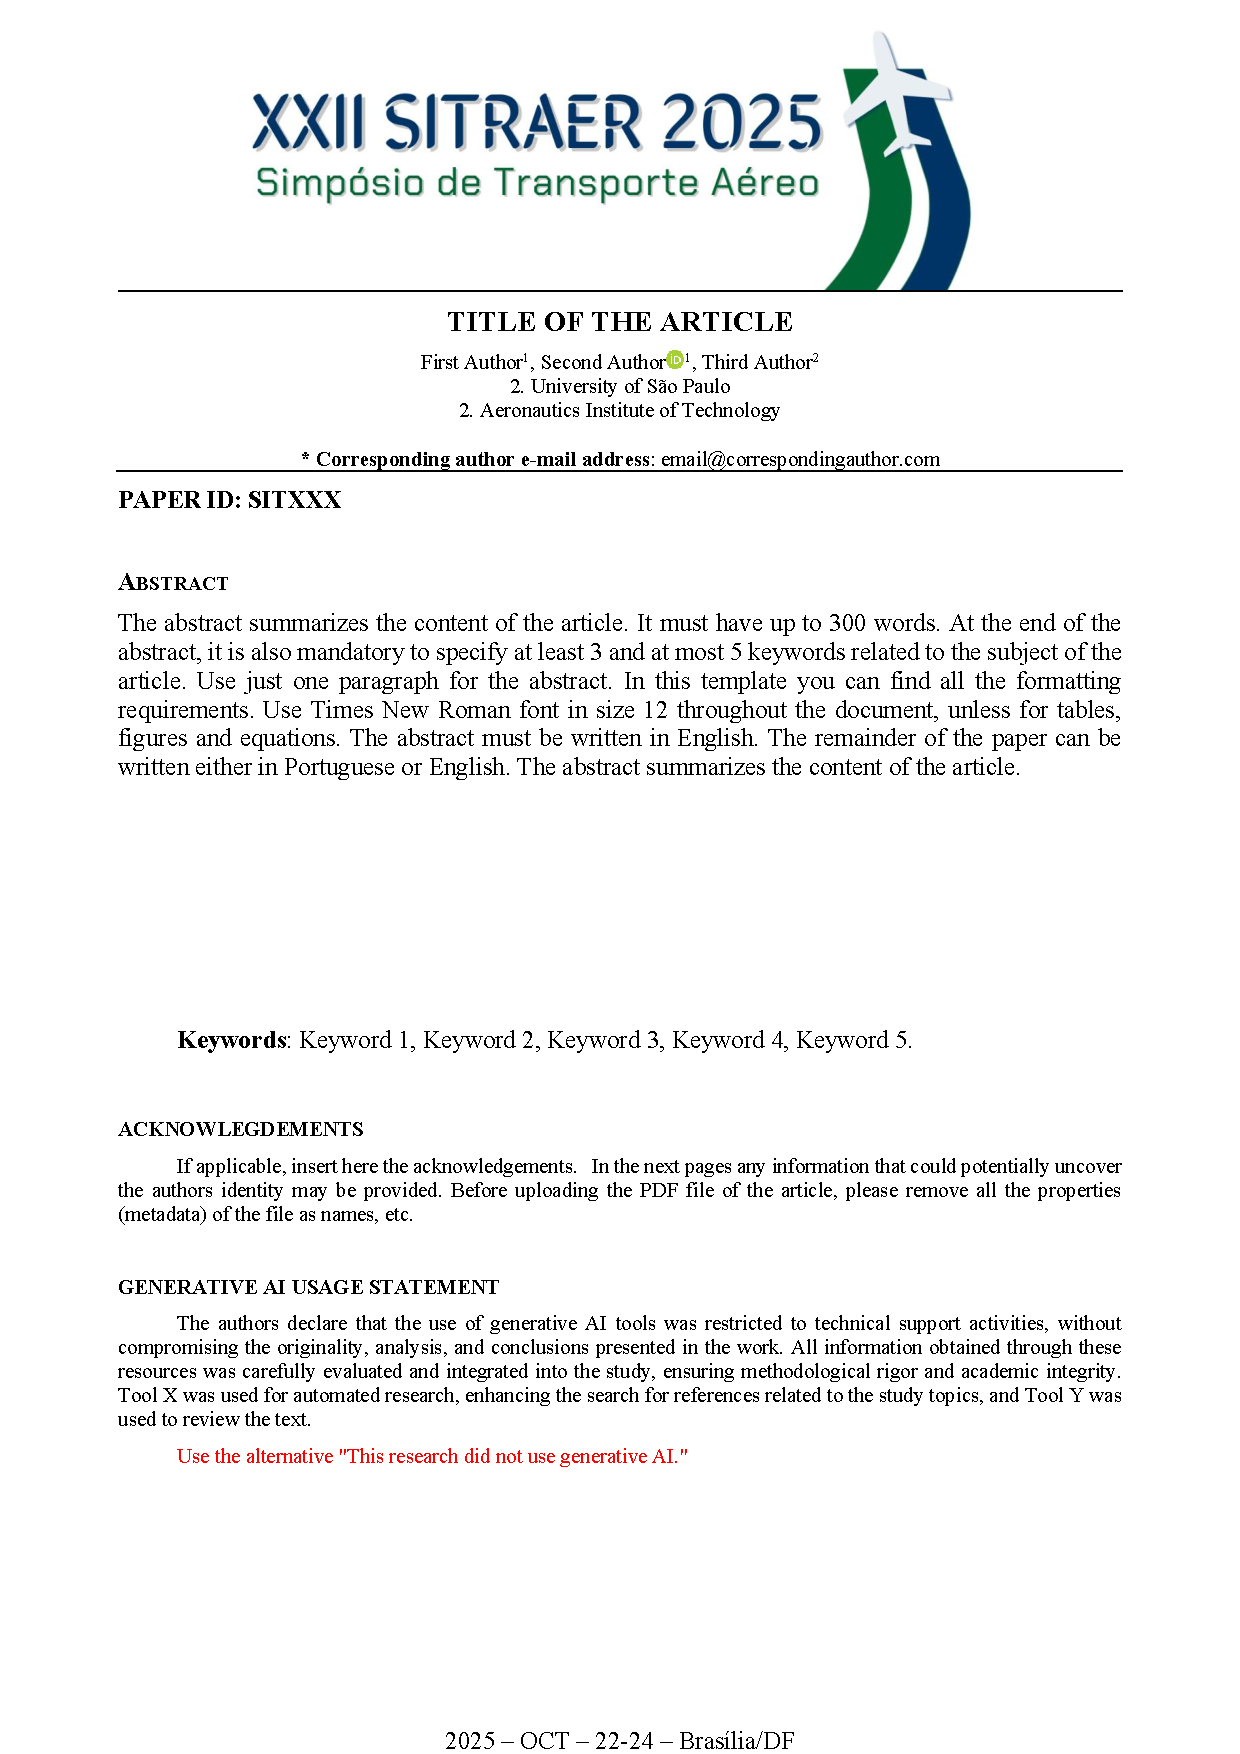
\includepdf[pages=-]{AneA/anexoA.pdf}





\chapter{Carta de Obstáculos de Aeródromo do SBSJ}\label{anexo:aoc}
Este anexo reproduz a Carta de Obstáculos de Aeródromo -- Tipo~A (AOC) do SBSJ, emenda AIRAC~2213, de 2022 \cite{decea2022aoc}, da qual foram extraídas as Figuras~\ref{fig:aoc-dist} e~\ref{fig:aoc-planta}.

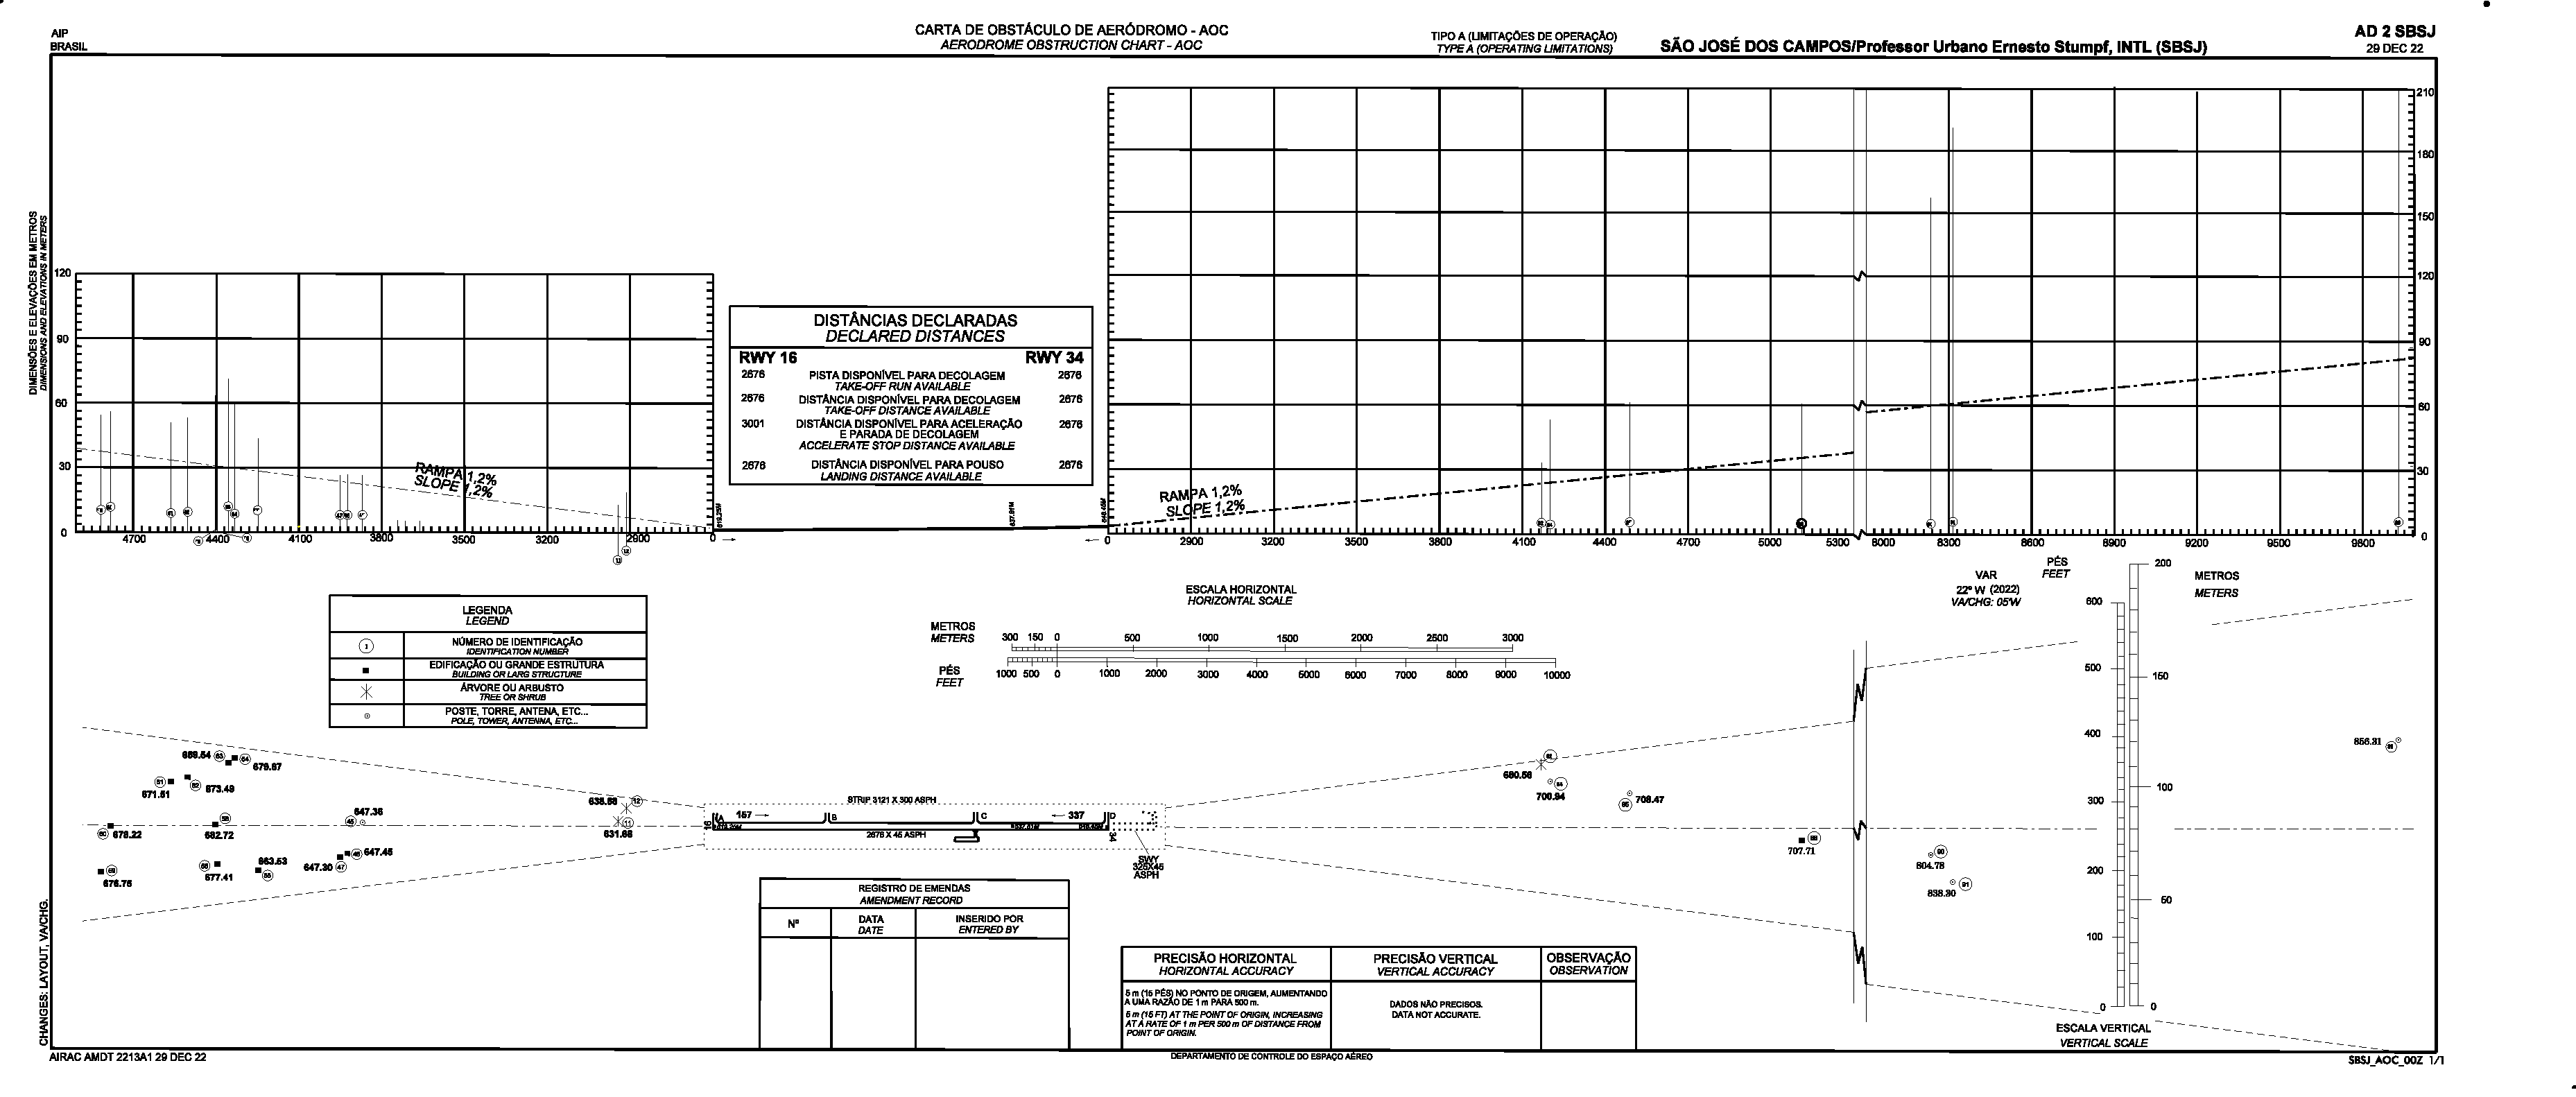
\includepdf[pages=-,landscape]{Anexos/sbsj_aoc_20221229.pdf}


\iffalse
%Glossário ------------------------------------------
\newcommand{\itaglosstitle}{%
    \iflanguage{portuguese}{Glossário}{Glossary}%
}
\chapter*{\itaglosstitle}
\addcontentsline{toc}{chapter}{\itaglosstitle}

\noindent
\textbf{Termo:} Definição.

%Folha de Registro do Documento ---------------------
\FRDitadata{DATA}
\FRDitadocnro{DCTA/ITA/TC-???/2026} % número solicitado à Biblioteca
\FRDitaorgaointerno{Instituto Tecnológico de Aeronáutica -- ITA}
\FRDitapalavrasautor{Informação aeronáutica; Aeroportos; Auditabilidade}
\FRDitapalavrasresult{PREENCHER}
\FRDitapalavraapresentacao{Trabalho de Graduação, ITA, São José dos Campos, 2026. \NumPenultimaPagina\ páginas.}
\FRDitaresumo{A informação aeronáutica sobre a infraestrutura de aeroportos chega aos usuários por meio de produtos oficiais, como a Publicação de Informação Aeronáutica e as cartas aeronáuticas, que apresentam o estado dos dados na data de efetividade de cada edição. 
Quando um valor muda entre edições, a mudança pode refletir um novo levantamento, uma obra ou uma correção. O produto publicado, porém, não informa qual foi a causa, quem a afirmou nem de quais premissas o novo valor depende. 
Este trabalho trata dessa lacuna de rastreabilidade, sem pretender verificar a exatidão das medições. 
Propõe-se uma arquitetura de dados para o lado ar de aeroportos baseada em \textit{event sourcing}, em que cada alteração é registrada como um evento acrescentado a um registro que não admite edição nem exclusão, com autor e causa, à maneira de um livro-razão contábil. 
Os valores que podem ser calculados, como comprimentos e distâncias declaradas, não são armazenados: são derivados das premissas no momento da consulta. 
A arquitetura foi implementada como biblioteca de código aberto e avaliada, segundo a pesquisa em ciência do design, por seis experimentos com dados reais da pista do Aeroporto de São José dos Campos, o primeiro deles de caracterização da lacuna, com critérios de aprovação definidos antes da execução. 
Os valores publicados foram recalculados dentro da precisão oficial, o estado dos dados em instantes passados foi reconstruído com a causa de cada alteração, as modificações feitas no meio do histórico foram detectadas e um verificador independente confirmou a integridade do registro sem recorrer à biblioteca. 
Conclui-se que, no caso estudado, a arquitetura torna esses dados rastreáveis e verificáveis, dentro de limites declarados: a auditabilidade é documental, e não da condição física da pista; a reescrita completa do histórico só é detectada por comparação com uma referência externa, que não foi implementada; a autoria é registrada, mas não autenticada; e os resultados provêm de um único estudo de caso.

\bigskip
\noindent\textbf{Palavras-chave:} Informação aeronáutica. Aeroportos.
Auditabilidade. \textit{Event sourcing}. Referenciamento linear.}
%  Nacional ou Internacional -- N/I ; Ostensivo, Reservado, Confidencial ou Secreto -- O/R/C/S
\FRDitaOpcoes{N}{O}
\itaFRD
\fi

\end{document}

%%% Template: Evandro José da Silva, Decio Yoshimoto (Dez 2024); versão Overleaf por
%%% Alejandro A. Rios Cruz, Saulo Gómez, Ocimar Santos.
%%% Overleaf: https://pt.overleaf.com/latex/templates/thesis-template-aeronautics-institute-of-technology-ita/yhfrqqydpygk
%%% GitHub:   https://github.com/AlejandroRios/Template_Thesis_ITA